\documentclass{article}
\usepackage[a4paper, margin=1in]{geometry} 
\usepackage{hyperref}
\usepackage{breakurl}
\usepackage{xurl}
\usepackage{amsmath}
\usepackage{graphicx}
\usepackage{listings}
\usepackage{xcolor}
\usepackage{pgf-pie}
\usepackage{float}
\usepackage{booktabs}
\usepackage{longtable} % Per tabelle che si estendono su più pagine
\usepackage{array}     % Per allineamento avanzato delle colonne
\usepackage{tabularx}  % Per tabelle che si adattano alla larghezza della pagina
\usepackage{caption}
\usepackage{colortbl} % Per colorare le righe della tabella
\usepackage{morewrites}
\usepackage{etex}



% Configura la distanza tra tabella e didascalia
\captionsetup{belowskip=12pt} % Imposta uno spazio di 12pt sotto la tabella

\definecolor{darkgreen}{rgb}{0.0, 0.5, 0.0} % Verde più scuro
\definecolor{darkviolet}{rgb}{0.58, 0.0, 0.83} % Viola più intenso
\definecolor{lightred}{rgb}{1.0, 0.8, 0.8}
\definecolor{lightyellow}{rgb}{1.0, 1.0, 0.8}
\definecolor{lightgreen}{rgb}{0.8, 1.0, 0.8}


\title{Report for Domain: edison.it}
\author{Generated by Apollo}
\date{\today}

\begin{document}

\maketitle
\clearpage

\tableofcontents  % Generates the table of contents

\clearpage

\section{Summary of Findings}

Below are some key statistics from the data provided:

\begin{itemize}
    \item \textbf{Number of IPs}: 90
    \item \textbf{Number of Domains}: 154
    \item \textbf{Number of Emails}: 16
    \item \textbf{Number of Resolved Hosts}: 52
    \item \textbf{Number of Mail Servers}: 4
    \item \textbf{Number of URLs}: 0
\end{itemize}

\clearpage

\section{IP Addresses found}

Below is the list of IP addresses found:


\begin{itemize}
    
        
            \item 151.22.39.45
        
            \item 151.22.38.13
        
            \item 204.246.191.61
        
            \item 52.211.124.234
        
            \item 195.103.103.30
        
            \item 212.73.193.150
        
            \item 89.197.73.20
        
            \item 62.94.137.201
        
            \item 213.217.29.85
        
            \item 3.64.78.167
        
            \item 151.22.38.14
        
            \item 151.22.38.130
        
            \item 3.121.19.218
        
            \item 185.91.71.118
        
            \item 94.124.69.67
        
            \item 62.94.137.182
        
            \item 0.0.0.0
        
            \item 51.75.86.118
        
            \item 54.192.76.24
        
            \item 37.72.32.254
        
            \item 151.22.38.175
        
            \item 3.120.219.35
        
            \item 37.72.32.222
        
            \item 52.51.233.170
        
            \item 108.138.192.49
        
            \item 54.192.76.85
        
            \item 151.22.38.156
        
            \item 51.178.13.239
        
            \item 151.22.39.54
        
            \item 51.91.24.51
        
            \item 212.35.216.126
        
            \item 151.22.39.9
        
            \item 40.126.32.129
        
            \item 109.168.22.86
        
            \item 93.186.249.30
        
            \item 46.28.2.183
        
            \item 62.94.137.206
        
            \item 95.174.28.207
        
            \item 108.157.194.127
        
            \item 151.22.38.131
        
            \item 151.22.39.6
        
            \item 151.22.39.122
        
            \item 52.50.23.25
        
            \item 83.211.69.255
        
            \item 3.126.218.72
        
            \item 51.15.59.206
        
            \item 151.22.38.152
        
            \item 151.22.39.18
        
            \item 195.231.62.154
        
            \item 52.49.152.75
        
            \item 35.156.181.89
        
            \item 93.186.242.241
        
            \item 156.54.148.62
        
            \item 204.246.191.51
        
            \item 37.72.32.244
        
            \item 52.213.159.238
        
            \item 54.192.76.55
        
            \item 40.126.32.6
        
            \item 51.38.105.34
        
            \item 3.126.233.235
        
            \item 54.192.76.109
        
            \item 52.98.242.232
        
            \item 151.22.38.214
        
            \item 40.87.138.215
        
            \item 18.202.92.68
        
            \item 151.22.39.38
        
            \item 204.246.191.9
        
            \item 151.22.38.234
        
            \item 34.248.167.34
        
            \item 137.135.246.66
        
            \item 151.22.39.27
        
            \item 54.76.95.70
        
            \item 109.168.22.85
        
            \item 151.22.38.133
        
            \item 63.33.242.246
        
            \item 62.94.137.200
        
            \item 151.22.38.140
        
            \item 13.74.182.99
        
            \item 3.125.77.225
        
            \item 151.101.65.195
        
            \item 204.246.191.8
        
            \item 162.55.172.85
        
            \item 151.22.38.70
        
            \item 151.22.39.19
        
            \item 37.72.32.255
        
            \item 151.101.1.195
        
            \item 94.127.86.211
        
            \item 18.195.121.173
        
            \item 151.22.38.198
        
            \item 151.22.38.155
        
    
\end{itemize}

\clearpage

\section{Domain found}

Below is the list of Domain found:

\begin{itemize}
    
        
            \item consipsl3.edison.it
        
            \item editoowanl01.corp.edison.it
        
            \item ediaw01.free.edison.it
        
            \item facilitysolutions.edison.it
        
            \item documentale-itg.edison.it
        
            \item bonus.edison.it
        
            \item edoc.edison.it
        
            \item gdc.edison.it
        
            \item gen-e.edison.it
        
            \item portaleproduttori2.edison.it
        
            \item webcon.edison.it
        
            \item vireoxmobile.edison.it
        
            \item da.edison.it
        
            \item cowprep.corp.edison.it
        
            \item hubatoa.edison.it
        
            \item crm.prep.edison.it
        
            \item enefcampus.edison.it
        
            \item uag.free.edison.it
        
            \item certauth.sso.edison.it
        
            \item desitest.corp.edison.it
        
            \item ediema.edison.it
        
            \item outlook.corp.edison.it
        
            \item portalesrm.edison.it
        
            \item mi045wlc5508dr.corp.edison.it
        
            \item nicesvil.edison.it
        
            \item password-reset.edison.it
        
            \item hubtest.edison.it
        
            \item efficienzaenergetica.edison.it
        
            \item open.edison.it
        
            \item dnf.edison.it
        
            \item cbctest.corp.edison.it
        
            \item *.edison.it
        
            \item eas.edison.it
        
            \item ediprdalvcms01.corp.edison.it
        
            \item extranet.edison.it
        
            \item editstpiteas01.corp.edison.it
        
            \item inge.edison.it
        
            \item trayport.edison.it
        
            \item collaudo-dof.edison.it
        
            \item mail.edison.it
        
            \item vpnclientleonardo.edison.it
        
            \item av.edison.it
        
            \item legacy.edison.it
        
            \item stories.efficienzaenergetica.edison.it
        
            \item mi045ise3305ced.corp.edison.it
        
            \item extranet2010.edison.it
        
            \item qlv.free.edison.it
        
            \item erm.corp.edison.it
        
            \item er-ta.edison.it
        
            \item wsnomitsrg.edison.it
        
            \item thorprep.corp.edison.it
        
            \item mi045ise3305dr.corp.edison.it
        
            \item fgt.egypt.edison.it
        
            \item smtppub.edison.it
        
            \item wsnomitsrgtest.edison.it
        
            \item niceprod.edison.it
        
            \item edireppiteas01.corp.edison.it
        
            \item vpn-fornitori.edison.it
        
            \item ebidtest.corp.edison.it
        
            \item enterpriseregistration.edison.it
        
            \item autodiscover.edison.it
        
            \item segnalazioni.edison.it
        
            \item edisonnextbrandcenter.edison.it
        
            \item cbc.corp.edison.it
        
            \item edito-test-01.corp.edison.it
        
            \item cmor.edison.it
        
            \item powerprocert.edison.it
        
            \item email.edison.it
        
            \item crmee.edison.it
        
            \item pec.edison.it
        
            \item stonesvil.edison.it
        
            \item hub.portal.edison.it
        
            \item hedgingportal.corp.edison.it
        
            \item free.edison.it
        
            \item thortestatoa.edison.it
        
            \item noi.edison.it
        
            \item hub.edison.it
        
            \item portaleproduttori1.edison.it
        
            \item adt.edison.it
        
            \item authsap.edison.it
        
            \item elearning.edison.it
        
            \item qvmobiletest.corp.edison.it
        
            \item admpowerprocert.edison.it
        
            \item gateway.edison.it
        
            \item fmw.edison.it
        
            \item indep2010.edison.it
        
            \item dep.edison.it
        
            \item chargeandgo.edison.it
        
            \item desi.corp.edison.it
        
            \item elp.edison.it
        
            \item monitoraggiomar.edison.it
        
            \item enterpriseregistration.egypt.edison.it
        
            \item daemobile.edison.it
        
            \item authsaptest.edison.it
        
            \item etools1.edison.it
        
            \item ediweb.edison.it
        
            \item powerpro.edison.it
        
            \item ediema01.corp.edison.it
        
            \item mi045wlc5508ced.corp.edison.it
        
            \item stonecert.edison.it
        
            \item corp.edison.it
        
            \item ssl.edison.it
        
            \item sip.edison.it
        
            \item collaudo-noi.edison.it
        
            \item sso.edison.it
        
            \item teleriscaldamento.edison.it
        
            \item ebid.corp.edison.it
        
            \item asid.edison.it
        
            \item lyncdiscover.edison.it
        
            \item admpowerpro.edison.it
        
            \item ediprdpiteas01.corp.edison.it
        
            \item enterpriseregistration.corp.edison.it
        
            \item lync.edison.it
        
            \item documentale-stoccaggio.edison.it
        
            \item indep.edison.it
        
            \item er.edison.it
        
            \item centraletorviscosa.edison.it
        
            \item edicerpiteas01.corp.edison.it
        
            \item edison.it
        
            \item ediprdenras11.corp.edison.it
        
            \item leonardo.edison.it
        
            \item energiachecambiatutto.edison.it
        
            \item vpnlondon.edison.it
        
            \item stone.edison.it
        
            \item pss.edison.it
        
            \item vpn.edison.it
        
            \item ssl-eesm-ot.edison.it
        
            \item ema.edison.it
        
            \item er-fa.edison.it
        
            \item edisonbrandcenter.edison.it
        
            \item 140anni.edison.it
        
            \item owebapp.edison.it
        
            \item areaclienti.prep.edison.it
        
            \item inwelldiary.edison.it
        
            \item lyncws.edison.it
        
            \item directorsdocuments.edison.it
        
            \item move.edison.it
        
            \item authsapdev.edison.it
        
            \item citrix.edison.it
        
            \item edisonfornature.edison.it
        
            \item portale.edison.it
        
            \item thorprod.corp.edison.it
        
            \item enterpriseregistration.fenice.edison.it
        
            \item dep2010.edison.it
        
            \item iag.free.edison.it
        
            \item etools2.edison.it
        
            \item mdm.free.edison.it
        
            \item elyx.edison.it
        
            \item softweb.edison.it
        
            \item dof.edison.it
        
            \item edisonmediacenter.edison.it
        
            \item monitoraggiomar-test.edison.it
        
            \item comparatoreofferte.edison.it
        
            \item spfk.edison.it
        
    
\end{itemize}

\clearpage


\section{URLs found}

Below is the list of URLs found:
\begin{itemize}
    
        \item No URLs found
    
\end{itemize}

\clearpage

\section{Domain Related to URLs Found}


\begin{itemize}
    \item No Domains or URLs found
\end{itemize}


\clearpage

\section{Emails found}

Below is the list of Emails found:

\begin{itemize}
    
        
            \item lorenzo.matucci@edison.it
        
            \item servizioclienti@edison.it
        
            \item staffqualifiche@edison.it
        
            \item edisonenergia\_faci@edison.it
        
            \item allacci\_subentri@edison.it
        
            \item cristina.parenti@edison.it
        
            \item hr.onboarding@edison.it
        
            \item ufficiostampa@edison.it
        
            \item elena.distaso@edison.it
        
            \item massimiliano.cicalese@edison.it
        
            \item lucia.caltagirone@edison.it
        
            \item edisonnext@pec.edison.it
        
            \item sostenibilita@edison.it
        
            \item edison@pec.edison.it
        
            \item supporto.fornitori@edison.it
        
            \item jane.doe@edison.it
        
    
\end{itemize}

\clearpage

\section{Resolved Hosts}

Below is a list of resolved hosts with their corresponding IP addresses:

\begin{itemize}
    
        
            \item \textbf{ 140anni.edison.it }: 108.157.194.127
        
            \item \textbf{ adt.edison.it }: 3.120.219.35
        
            \item \textbf{ authsap.edison.it }: 3.125.77.225
        
            \item \textbf{ authsapdev.edison.it }: 3.125.77.225
        
            \item \textbf{ autodiscover.edison.it }: 52.98.242.232
        
            \item \textbf{ centraletorviscosa.edison.it }: 35.156.181.89
        
            \item \textbf{ chargeandgo.edison.it }: 109.168.22.86
        
            \item \textbf{ comparatoreofferte.edison.it }: 3.120.219.35
        
            \item \textbf{ consipsl3.edison.it }: 156.54.148.62
        
            \item \textbf{ crm.prep.edison.it }: 151.22.38.152
        
            \item \textbf{ crmee.edison.it }: 151.22.38.156
        
            \item \textbf{ daemobile.edison.it }: 151.22.38.140
        
            \item \textbf{ directorsdocuments.edison.it }: 40.87.138.215
        
            \item \textbf{ dnf.edison.it }: 108.138.192.49
        
            \item \textbf{ ediema.edison.it }: 151.22.38.234
        
            \item \textbf{ edison.it }: 51.38.105.34
        
            \item \textbf{ edisonbrandcenter.edison.it }: 46.28.2.183
        
            \item \textbf{ edisonfornature.edison.it }: 0.0.0.0
        
            \item \textbf{ edisonmediacenter.edison.it }: 46.28.2.183
        
            \item \textbf{ edisonnextbrandcenter.edison.it }: 46.28.2.183
        
            \item \textbf{ efficienzaenergetica.edison.it }: 54.76.95.70
        
            \item \textbf{ elearning.edison.it }: 94.124.69.67
        
            \item \textbf{ elp.edison.it }: 35.156.181.89
        
            \item \textbf{ ema.edison.it }: 3.126.233.235
        
            \item \textbf{ enefcampus.edison.it }: 51.91.24.51
        
            \item \textbf{ enterpriseregistration.corp.edison.it }: 40.126.32.6
        
            \item \textbf{ enterpriseregistration.edison.it }: 40.126.32.6
        
            \item \textbf{ enterpriseregistration.fenice.edison.it }: 40.126.32.129
        
            \item \textbf{ er-fa.edison.it }: 37.72.32.255
        
            \item \textbf{ er-ta.edison.it }: 37.72.32.222
        
            \item \textbf{ er.edison.it }: 37.72.32.254
        
            \item \textbf{ fmw.edison.it }: 151.22.39.54
        
            \item \textbf{ gateway.edison.it }: 151.22.38.133
        
            \item \textbf{ gen-e.edison.it }: 93.186.242.241
        
            \item \textbf{ iag.free.edison.it }: 151.22.38.70
        
            \item \textbf{ mail.edison.it }: 151.22.38.175
        
            \item \textbf{ monitoraggiomar-test.edison.it }: 63.33.242.246
        
            \item \textbf{ monitoraggiomar.edison.it }: 34.248.167.34
        
            \item \textbf{ open.edison.it }: 0.0.0.0
        
            \item \textbf{ powerpro.edison.it }: 35.156.181.89
        
            \item \textbf{ pss.edison.it }: 151.22.38.155
        
            \item \textbf{ segnalazioni.edison.it }: 95.174.28.207
        
            \item \textbf{ smtppub.edison.it }: 151.22.38.131
        
            \item \textbf{ ssl-eesm-ot.edison.it }: 151.22.39.122
        
            \item \textbf{ ssl.edison.it }: 151.22.38.13
        
            \item \textbf{ stories.efficienzaenergetica.edison.it }: 151.101.65.195
        
            \item \textbf{ vireoxmobile.edison.it }: 37.72.32.244
        
            \item \textbf{ vpn-fornitori.edison.it }: 151.22.38.133
        
            \item \textbf{ vpn.edison.it }: 151.22.38.14
        
            \item \textbf{ vpnclientleonardo.edison.it }: 195.231.62.154
        
            \item \textbf{ wsnomitsrg.edison.it }: 3.121.19.218
        
            \item \textbf{ wsnomitsrgtest.edison.it }: 18.195.121.173
        
    
\end{itemize}

\clearpage

\section{Server Mail found}

Below is the list of Mail Server found:

\begin{itemize}
    
        
            \item 213.217.29.85
        
            \item 185.91.71.118
        
            \item edison2.esvacloud.com.
        
            \item edison.esvacloud.com.
        
    
\end{itemize}

\clearpage

\section{Pie Chart of Vulnerabilities}

\noindent Pie chart showing the distribution of vulnerabilities for the domain \ttfamily edison.it:


\begin{figure}[H]
    \centering
    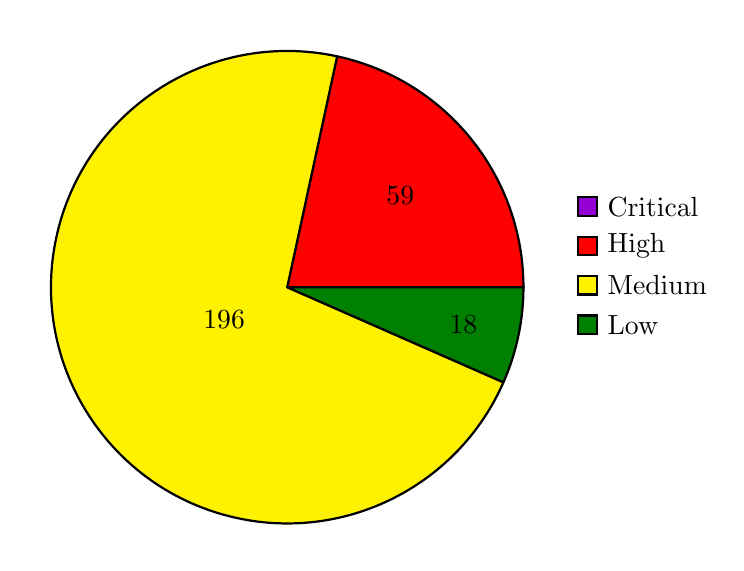
\begin{tikzpicture}
        \pie[
            color={darkviolet, red, yellow, darkgreen},
            text=legend,
            radius=3,
            sum=273
        ]
        {
            0/Critical,
            59/High,
            196/Medium,
            18/Low
        }
    \end{tikzpicture}
\end{figure}


\clearpage

\section{Vulnerability Summary per IP}

\noindent The table below shows the number of critical, high, medium, and low vulnerabilities for each IP, ordered by the number of vulnerabilities (first by critical, then high, medium, and low):

\begin{longtable}{|>{\raggedright\arraybackslash}p{3cm}|c|c|c|c|}
    \hline
    \textbf{IP Address} & \textbf{Critical} & \textbf{High} & \textbf{Medium} & \textbf{Low} \\
    \hline
    \endfirsthead
    \hline
    \textbf{IP Address} & \textbf{Critical} & \textbf{High} & \textbf{Medium} & \textbf{Low} \\
    \hline
    \endhead
    \hline
    \endfoot
    \endlastfoot
    
    
    
    \rowcolor{lightred} % Righe con critical o high evidenziate in rosso
    
    109.168.22.85 & 0 & 27 & 73 & 4 \\
    \hline
    
    
    \rowcolor{lightred} % Righe con critical o high evidenziate in rosso
    
    54.76.95.70 & 0 & 26 & 106 & 10 \\
    \hline
    
    
    \rowcolor{lightred} % Righe con critical o high evidenziate in rosso
    
    212.35.216.126 & 0 & 6 & 14 & 4 \\
    \hline
    
    
    \rowcolor{lightyellow} % Righe con medium o low evidenziate in giallo
    
    109.168.22.86 & 0 & 0 & 3 & 0 \\
    \hline
    
    
    \rowcolor{lightgreen} % Righe senza vulnerabilità evidenziate in verde
    
    62.94.137.182 & 0 & 0 & 0 & 0 \\
    \hline
    
    
    \rowcolor{lightgreen} % Righe senza vulnerabilità evidenziate in verde
    
    3.126.233.235 & 0 & 0 & 0 & 0 \\
    \hline
    
    
    \rowcolor{lightgreen} % Righe senza vulnerabilità evidenziate in verde
    
    93.186.242.241 & 0 & 0 & 0 & 0 \\
    \hline
    
    
    \rowcolor{lightgreen} % Righe senza vulnerabilità evidenziate in verde
    
    3.125.77.225 & 0 & 0 & 0 & 0 \\
    \hline
    
    
    \rowcolor{lightgreen} % Righe senza vulnerabilità evidenziate in verde
    
    151.101.65.195 & 0 & 0 & 0 & 0 \\
    \hline
    
    
    \rowcolor{lightgreen} % Righe senza vulnerabilità evidenziate in verde
    
    37.72.32.255 & 0 & 0 & 0 & 0 \\
    \hline
    
    
    \rowcolor{lightgreen} % Righe senza vulnerabilità evidenziate in verde
    
    54.192.76.24 & 0 & 0 & 0 & 0 \\
    \hline
    
    
    \rowcolor{lightgreen} % Righe senza vulnerabilità evidenziate in verde
    
    18.202.92.68 & 0 & 0 & 0 & 0 \\
    \hline
    
    
    \rowcolor{lightgreen} % Righe senza vulnerabilità evidenziate in verde
    
    151.22.38.13 & 0 & 0 & 0 & 0 \\
    \hline
    
    
    \rowcolor{lightgreen} % Righe senza vulnerabilità evidenziate in verde
    
    156.54.148.62 & 0 & 0 & 0 & 0 \\
    \hline
    
    
    \rowcolor{lightgreen} % Righe senza vulnerabilità evidenziate in verde
    
    37.72.32.222 & 0 & 0 & 0 & 0 \\
    \hline
    
    
    \rowcolor{lightgreen} % Righe senza vulnerabilità evidenziate in verde
    
    52.98.242.232 & 0 & 0 & 0 & 0 \\
    \hline
    
    
    \rowcolor{lightgreen} % Righe senza vulnerabilità evidenziate in verde
    
    3.64.78.167 & 0 & 0 & 0 & 0 \\
    \hline
    
    
    \rowcolor{lightgreen} % Righe senza vulnerabilità evidenziate in verde
    
    52.211.124.234 & 0 & 0 & 0 & 0 \\
    \hline
    
    
    \rowcolor{lightgreen} % Righe senza vulnerabilità evidenziate in verde
    
    151.101.1.195 & 0 & 0 & 0 & 0 \\
    \hline
    
    
    \rowcolor{lightgreen} % Righe senza vulnerabilità evidenziate in verde
    
    51.178.13.239 & 0 & 0 & 0 & 0 \\
    \hline
    
    
    \rowcolor{lightgreen} % Righe senza vulnerabilità evidenziate in verde
    
    3.120.219.35 & 0 & 0 & 0 & 0 \\
    \hline
    
    
    \rowcolor{lightgreen} % Righe senza vulnerabilità evidenziate in verde
    
    46.28.2.183 & 0 & 0 & 0 & 0 \\
    \hline
    
    
    \rowcolor{lightgreen} % Righe senza vulnerabilità evidenziate in verde
    
    89.197.73.20 & 0 & 0 & 0 & 0 \\
    \hline
    
    
    \rowcolor{lightgreen} % Righe senza vulnerabilità evidenziate in verde
    
    37.72.32.244 & 0 & 0 & 0 & 0 \\
    \hline
    
    
    \rowcolor{lightgreen} % Righe senza vulnerabilità evidenziate in verde
    
    151.22.39.122 & 0 & 0 & 0 & 0 \\
    \hline
    
    
    \rowcolor{lightgreen} % Righe senza vulnerabilità evidenziate in verde
    
    151.22.38.133 & 0 & 0 & 0 & 0 \\
    \hline
    
    
    \rowcolor{lightgreen} % Righe senza vulnerabilità evidenziate in verde
    
    151.22.38.14 & 0 & 0 & 0 & 0 \\
    \hline
    
    
    \rowcolor{lightgreen} % Righe senza vulnerabilità evidenziate in verde
    
    62.94.137.206 & 0 & 0 & 0 & 0 \\
    \hline
    
    
    \rowcolor{lightgreen} % Righe senza vulnerabilità evidenziate in verde
    
    62.94.137.201 & 0 & 0 & 0 & 0 \\
    \hline
    
    
    \rowcolor{lightgreen} % Righe senza vulnerabilità evidenziate in verde
    
    35.156.181.89 & 0 & 0 & 0 & 0 \\
    \hline
    
    
    \rowcolor{lightgreen} % Righe senza vulnerabilità evidenziate in verde
    
    213.217.29.85 & 0 & 0 & 0 & 0 \\
    \hline
    
    
    \rowcolor{lightgreen} % Righe senza vulnerabilità evidenziate in verde
    
    94.124.69.67 & 0 & 0 & 0 & 0 \\
    \hline
    
    
    \rowcolor{lightgreen} % Righe senza vulnerabilità evidenziate in verde
    
    52.50.23.25 & 0 & 0 & 0 & 0 \\
    \hline
    
    
    \rowcolor{lightgreen} % Righe senza vulnerabilità evidenziate in verde
    
    185.91.71.118 & 0 & 0 & 0 & 0 \\
    \hline
    
    \caption{Number of vulnerabilities per IP, sorted by severity.} \\
\end{longtable}

\clearpage

\section{Shodan Results for IP Addresses}

Below is the detailed report of vulnerabilities and services for each IP address:






\subsection{IP Address: 109.168.22.85}

\begin{itemize}
    \item \textbf{Organization}: SEH SRL . - 6275212
    \item \textbf{Operating System}:  Ubuntu 
    \item \textbf{Critical Vulnerabilities}: 0
    \item \textbf{High Vulnerabilities}: 27
    \item \textbf{Medium Vulnerabilities}: 73
    \item \textbf{Low Vulnerabilities}: 4
    \item \textbf{Total Vulnerabilities}: 104
\end{itemize}

\subsubsection*{Services Running on IP Address}

\begin{itemize}
    
        \item \textbf{Service}: nginx
        \begin{itemize}
            \item \textbf{Port}: 80
            \item \textbf{Version}:  1.14.0 
            \item \textbf{Location}: \href{ https://demo-ricaricaev.seh.it/ }{ https://demo-ricaricaev.seh.it/ }
        \end{itemize}
    
        \item \textbf{Service}: nginx
        \begin{itemize}
            \item \textbf{Port}: 443
            \item \textbf{Version}:  1.14.0 
            \item \textbf{Location}: \href{ / }{ / }
        \end{itemize}
    
        \item \textbf{Service}: N/A
        \begin{itemize}
            \item \textbf{Port}: 5060
            \item \textbf{Version}:  N/A 
            \item \textbf{Location}: \href{  }{  }
        \end{itemize}
    
        \item \textbf{Service}: Apache httpd
        \begin{itemize}
            \item \textbf{Port}: 8000
            \item \textbf{Version}:  2.4.29 
            \item \textbf{Location}: \href{  }{  }
        \end{itemize}
    
        \item \textbf{Service}: nginx
        \begin{itemize}
            \item \textbf{Port}: 8080
            \item \textbf{Version}:  1.14.0 
            \item \textbf{Location}: \href{ https://demo-ricaricaev.seh.it/ }{ https://demo-ricaricaev.seh.it/ }
        \end{itemize}
    
        \item \textbf{Service}: nginx
        \begin{itemize}
            \item \textbf{Port}: 8443
            \item \textbf{Version}:  1.14.0 
            \item \textbf{Location}: \href{ / }{ / }
        \end{itemize}
    
\end{itemize}


\subsubsection*{Vulnerabilities Found}

\begin{itemize}
    
        \item \textbf{Vulnerability}: CVE-2023-44487
        \begin{itemize}
            \item \textbf{CVSS Score}:  N/A 
            \item \textbf{Description}:
            \parbox[t]{0.9\linewidth}{
                \ttfamily The HTTP/2 protocol allows a denial of service (server resource consumption) because request cancellation can reset many streams quickly, as exploited in the wild in August through October 2023.
            }
        \end{itemize}
    
        \item \textbf{Vulnerability}: CVE-2019-9516
        \begin{itemize}
            \item \textbf{CVSS Score}:  6.8 
            \item \textbf{Description}:
            \parbox[t]{0.9\linewidth}{
                \ttfamily Some HTTP/2 implementations are vulnerable to a header leak, potentially leading to a denial of service. The attacker sends a stream of headers with a 0-length header name and 0-length header value, optionally Huffman encoded into 1-byte or greater headers. Some implementations allocate memory for these headers and keep the allocation alive until the session dies. This can consume excess memory.
            }
        \end{itemize}
    
        \item \textbf{Vulnerability}: CVE-2019-9513
        \begin{itemize}
            \item \textbf{CVSS Score}:  7.8 
            \item \textbf{Description}:
            \parbox[t]{0.9\linewidth}{
                \ttfamily Some HTTP/2 implementations are vulnerable to resource loops, potentially leading to a denial of service. The attacker creates multiple request streams and continually shuffles the priority of the streams in a way that causes substantial churn to the priority tree. This can consume excess CPU.
            }
        \end{itemize}
    
        \item \textbf{Vulnerability}: CVE-2019-9511
        \begin{itemize}
            \item \textbf{CVSS Score}:  7.8 
            \item \textbf{Description}:
            \parbox[t]{0.9\linewidth}{
                \ttfamily Some HTTP/2 implementations are vulnerable to window size manipulation and stream prioritization manipulation, potentially leading to a denial of service. The attacker requests a large amount of data from a specified resource over multiple streams. They manipulate window size and stream priority to force the server to queue the data in 1-byte chunks. Depending on how efficiently this data is queued, this can consume excess CPU, memory, or both.
            }
        \end{itemize}
    
        \item \textbf{Vulnerability}: CVE-2018-16843
        \begin{itemize}
            \item \textbf{CVSS Score}:  7.8 
            \item \textbf{Description}:
            \parbox[t]{0.9\linewidth}{
                \ttfamily nginx before versions 1.15.6 and 1.14.1 has a vulnerability in the implementation of HTTP/2 that can allow for excessive memory consumption. This issue affects nginx compiled with the ngx\_http\_v2\_module (not compiled by default) if the 'http2' option of the 'listen' directive is used in a configuration file.
            }
        \end{itemize}
    
        \item \textbf{Vulnerability}: CVE-2021-23017
        \begin{itemize}
            \item \textbf{CVSS Score}:  6.8 
            \item \textbf{Description}:
            \parbox[t]{0.9\linewidth}{
                \ttfamily A security issue in nginx resolver was identified, which might allow an attacker who is able to forge UDP packets from the DNS server to cause 1-byte memory overwrite, resulting in worker process crash or potential other impact.
            }
        \end{itemize}
    
        \item \textbf{Vulnerability}: CVE-2021-3618
        \begin{itemize}
            \item \textbf{CVSS Score}:  5.8 
            \item \textbf{Description}:
            \parbox[t]{0.9\linewidth}{
                \ttfamily ALPACA is an application layer protocol content confusion attack, exploiting TLS servers implementing different protocols but using compatible certificates, such as multi-domain or wildcard certificates. A MiTM attacker having access to victim's traffic at the TCP/IP layer can redirect traffic from one subdomain to another, resulting in a valid TLS session. This breaks the authentication of TLS and cross-protocol attacks may be possible where the behavior of one protocol service may compromise the other at the application layer.
            }
        \end{itemize}
    
        \item \textbf{Vulnerability}: CVE-2019-20372
        \begin{itemize}
            \item \textbf{CVSS Score}:  4.3 
            \item \textbf{Description}:
            \parbox[t]{0.9\linewidth}{
                \ttfamily NGINX before 1.17.7, with certain error\_page configurations, allows HTTP request smuggling, as demonstrated by the ability of an attacker to read unauthorized web pages in environments where NGINX is being fronted by a load balancer.
            }
        \end{itemize}
    
        \item \textbf{Vulnerability}: CVE-2018-16844
        \begin{itemize}
            \item \textbf{CVSS Score}:  7.8 
            \item \textbf{Description}:
            \parbox[t]{0.9\linewidth}{
                \ttfamily nginx before versions 1.15.6 and 1.14.1 has a vulnerability in the implementation of HTTP/2 that can allow for excessive CPU usage. This issue affects nginx compiled with the ngx\_http\_v2\_module (not compiled by default) if the 'http2' option of the 'listen' directive is used in a configuration file.
            }
        \end{itemize}
    
        \item \textbf{Vulnerability}: CVE-2018-16845
        \begin{itemize}
            \item \textbf{CVSS Score}:  5.8 
            \item \textbf{Description}:
            \parbox[t]{0.9\linewidth}{
                \ttfamily nginx before versions 1.15.6, 1.14.1 has a vulnerability in the ngx\_http\_mp4\_module, which might allow an attacker to cause infinite loop in a worker process, cause a worker process crash, or might result in worker process memory disclosure by using a specially crafted mp4 file. The issue only affects nginx if it is built with the ngx\_http\_mp4\_module (the module is not built by default) and the .mp4. directive is used in the configuration file. Further, the attack is only possible if an attacker is able to trigger processing of a specially crafted mp4 file with the ngx\_http\_mp4\_module.
            }
        \end{itemize}
    
        \item \textbf{Vulnerability}: CVE-2023-44487
        \begin{itemize}
            \item \textbf{CVSS Score}:  N/A 
            \item \textbf{Description}:
            \parbox[t]{0.9\linewidth}{
                \ttfamily The HTTP/2 protocol allows a denial of service (server resource consumption) because request cancellation can reset many streams quickly, as exploited in the wild in August through October 2023.
            }
        \end{itemize}
    
        \item \textbf{Vulnerability}: CVE-2018-16844
        \begin{itemize}
            \item \textbf{CVSS Score}:  7.8 
            \item \textbf{Description}:
            \parbox[t]{0.9\linewidth}{
                \ttfamily nginx before versions 1.15.6 and 1.14.1 has a vulnerability in the implementation of HTTP/2 that can allow for excessive CPU usage. This issue affects nginx compiled with the ngx\_http\_v2\_module (not compiled by default) if the 'http2' option of the 'listen' directive is used in a configuration file.
            }
        \end{itemize}
    
        \item \textbf{Vulnerability}: CVE-2019-11358
        \begin{itemize}
            \item \textbf{CVSS Score}:  4.3 
            \item \textbf{Description}:
            \parbox[t]{0.9\linewidth}{
                \ttfamily jQuery before 3.4.0, as used in Drupal, Backdrop CMS, and other products, mishandles jQuery.extend(true, \{\}, ...) because of Object.prototype pollution. If an unsanitized source object contained an enumerable \_\_proto\_\_ property, it could extend the native Object.prototype.
            }
        \end{itemize}
    
        \item \textbf{Vulnerability}: CVE-2019-9516
        \begin{itemize}
            \item \textbf{CVSS Score}:  6.8 
            \item \textbf{Description}:
            \parbox[t]{0.9\linewidth}{
                \ttfamily Some HTTP/2 implementations are vulnerable to a header leak, potentially leading to a denial of service. The attacker sends a stream of headers with a 0-length header name and 0-length header value, optionally Huffman encoded into 1-byte or greater headers. Some implementations allocate memory for these headers and keep the allocation alive until the session dies. This can consume excess memory.
            }
        \end{itemize}
    
        \item \textbf{Vulnerability}: CVE-2019-9513
        \begin{itemize}
            \item \textbf{CVSS Score}:  7.8 
            \item \textbf{Description}:
            \parbox[t]{0.9\linewidth}{
                \ttfamily Some HTTP/2 implementations are vulnerable to resource loops, potentially leading to a denial of service. The attacker creates multiple request streams and continually shuffles the priority of the streams in a way that causes substantial churn to the priority tree. This can consume excess CPU.
            }
        \end{itemize}
    
        \item \textbf{Vulnerability}: CVE-2019-9511
        \begin{itemize}
            \item \textbf{CVSS Score}:  7.8 
            \item \textbf{Description}:
            \parbox[t]{0.9\linewidth}{
                \ttfamily Some HTTP/2 implementations are vulnerable to window size manipulation and stream prioritization manipulation, potentially leading to a denial of service. The attacker requests a large amount of data from a specified resource over multiple streams. They manipulate window size and stream priority to force the server to queue the data in 1-byte chunks. Depending on how efficiently this data is queued, this can consume excess CPU, memory, or both.
            }
        \end{itemize}
    
        \item \textbf{Vulnerability}: CVE-2018-16843
        \begin{itemize}
            \item \textbf{CVSS Score}:  7.8 
            \item \textbf{Description}:
            \parbox[t]{0.9\linewidth}{
                \ttfamily nginx before versions 1.15.6 and 1.14.1 has a vulnerability in the implementation of HTTP/2 that can allow for excessive memory consumption. This issue affects nginx compiled with the ngx\_http\_v2\_module (not compiled by default) if the 'http2' option of the 'listen' directive is used in a configuration file.
            }
        \end{itemize}
    
        \item \textbf{Vulnerability}: CVE-2021-23017
        \begin{itemize}
            \item \textbf{CVSS Score}:  6.8 
            \item \textbf{Description}:
            \parbox[t]{0.9\linewidth}{
                \ttfamily A security issue in nginx resolver was identified, which might allow an attacker who is able to forge UDP packets from the DNS server to cause 1-byte memory overwrite, resulting in worker process crash or potential other impact.
            }
        \end{itemize}
    
        \item \textbf{Vulnerability}: CVE-2018-16845
        \begin{itemize}
            \item \textbf{CVSS Score}:  5.8 
            \item \textbf{Description}:
            \parbox[t]{0.9\linewidth}{
                \ttfamily nginx before versions 1.15.6, 1.14.1 has a vulnerability in the ngx\_http\_mp4\_module, which might allow an attacker to cause infinite loop in a worker process, cause a worker process crash, or might result in worker process memory disclosure by using a specially crafted mp4 file. The issue only affects nginx if it is built with the ngx\_http\_mp4\_module (the module is not built by default) and the .mp4. directive is used in the configuration file. Further, the attack is only possible if an attacker is able to trigger processing of a specially crafted mp4 file with the ngx\_http\_mp4\_module.
            }
        \end{itemize}
    
        \item \textbf{Vulnerability}: CVE-2021-3618
        \begin{itemize}
            \item \textbf{CVSS Score}:  5.8 
            \item \textbf{Description}:
            \parbox[t]{0.9\linewidth}{
                \ttfamily ALPACA is an application layer protocol content confusion attack, exploiting TLS servers implementing different protocols but using compatible certificates, such as multi-domain or wildcard certificates. A MiTM attacker having access to victim's traffic at the TCP/IP layer can redirect traffic from one subdomain to another, resulting in a valid TLS session. This breaks the authentication of TLS and cross-protocol attacks may be possible where the behavior of one protocol service may compromise the other at the application layer.
            }
        \end{itemize}
    
        \item \textbf{Vulnerability}: CVE-2019-20372
        \begin{itemize}
            \item \textbf{CVSS Score}:  4.3 
            \item \textbf{Description}:
            \parbox[t]{0.9\linewidth}{
                \ttfamily NGINX before 1.17.7, with certain error\_page configurations, allows HTTP request smuggling, as demonstrated by the ability of an attacker to read unauthorized web pages in environments where NGINX is being fronted by a load balancer.
            }
        \end{itemize}
    
        \item \textbf{Vulnerability}: CVE-2020-11022
        \begin{itemize}
            \item \textbf{CVSS Score}:  4.3 
            \item \textbf{Description}:
            \parbox[t]{0.9\linewidth}{
                \ttfamily In jQuery versions greater than or equal to 1.2 and before 3.5.0, passing HTML from untrusted sources - even after sanitizing it - to one of jQuery's DOM manipulation methods (i.e. .html(), .append(), and others) may execute untrusted code. This problem is patched in jQuery 3.5.0.
            }
        \end{itemize}
    
        \item \textbf{Vulnerability}: CVE-2020-11023
        \begin{itemize}
            \item \textbf{CVSS Score}:  4.3 
            \item \textbf{Description}:
            \parbox[t]{0.9\linewidth}{
                \ttfamily In jQuery versions greater than or equal to 1.0.3 and before 3.5.0, passing HTML containing <option> elements from untrusted sources - even after sanitizing it - to one of jQuery's DOM manipulation methods (i.e. .html(), .append(), and others) may execute untrusted code. This problem is patched in jQuery 3.5.0.
            }
        \end{itemize}
    
        \item \textbf{Vulnerability}: CVE-2019-0220
        \begin{itemize}
            \item \textbf{CVSS Score}:  5 
            \item \textbf{Description}:
            \parbox[t]{0.9\linewidth}{
                \ttfamily A vulnerability was found in Apache HTTP Server 2.4.0 to 2.4.38. When the path component of a request URL contains multiple consecutive slashes ('/'), directives such as LocationMatch and RewriteRule must account for duplicates in regular expressions while other aspects of the servers processing will implicitly collapse them.
            }
        \end{itemize}
    
        \item \textbf{Vulnerability}: CVE-2011-2688
        \begin{itemize}
            \item \textbf{CVSS Score}:  7.5 
            \item \textbf{Description}:
            \parbox[t]{0.9\linewidth}{
                \ttfamily SQL injection vulnerability in mysql/mysql-auth.pl in the mod\_authnz\_external module 3.2.5 and earlier for the Apache HTTP Server allows remote attackers to execute arbitrary SQL commands via the user field.
            }
        \end{itemize}
    
        \item \textbf{Vulnerability}: CVE-2013-2765
        \begin{itemize}
            \item \textbf{CVSS Score}:  5 
            \item \textbf{Description}:
            \parbox[t]{0.9\linewidth}{
                \ttfamily The ModSecurity module before 2.7.4 for the Apache HTTP Server allows remote attackers to cause a denial of service (NULL pointer dereference, process crash, and disk consumption) via a POST request with a large body and a crafted Content-Type header.
            }
        \end{itemize}
    
        \item \textbf{Vulnerability}: CVE-2020-1934
        \begin{itemize}
            \item \textbf{CVSS Score}:  5 
            \item \textbf{Description}:
            \parbox[t]{0.9\linewidth}{
                \ttfamily In Apache HTTP Server 2.4.0 to 2.4.41, mod\_proxy\_ftp may use uninitialized memory when proxying to a malicious FTP server.
            }
        \end{itemize}
    
        \item \textbf{Vulnerability}: CVE-2018-17189
        \begin{itemize}
            \item \textbf{CVSS Score}:  5 
            \item \textbf{Description}:
            \parbox[t]{0.9\linewidth}{
                \ttfamily In Apache HTTP server versions 2.4.37 and prior, by sending request bodies in a slow loris way to plain resources, the h2 stream for that request unnecessarily occupied a server thread cleaning up that incoming data. This affects only HTTP/2 (mod\_http2) connections.
            }
        \end{itemize}
    
        \item \textbf{Vulnerability}: CVE-2021-34798
        \begin{itemize}
            \item \textbf{CVSS Score}:  5 
            \item \textbf{Description}:
            \parbox[t]{0.9\linewidth}{
                \ttfamily Malformed requests may cause the server to dereference a NULL pointer. This issue affects Apache HTTP Server 2.4.48 and earlier.
            }
        \end{itemize}
    
        \item \textbf{Vulnerability}: CVE-2020-35452
        \begin{itemize}
            \item \textbf{CVSS Score}:  6.8 
            \item \textbf{Description}:
            \parbox[t]{0.9\linewidth}{
                \ttfamily Apache HTTP Server versions 2.4.0 to 2.4.46 A specially crafted Digest nonce can cause a stack overflow in mod\_auth\_digest. There is no report of this overflow being exploitable, nor the Apache HTTP Server team could create one, though some particular compiler and/or compilation option might make it possible, with limited consequences anyway due to the size (a single byte) and the value (zero byte) of the overflow
            }
        \end{itemize}
    
        \item \textbf{Vulnerability}: CVE-2022-29404
        \begin{itemize}
            \item \textbf{CVSS Score}:  5 
            \item \textbf{Description}:
            \parbox[t]{0.9\linewidth}{
                \ttfamily In Apache HTTP Server 2.4.53 and earlier, a malicious request to a lua script that calls r:parsebody(0) may cause a denial of service due to no default limit on possible input size.
            }
        \end{itemize}
    
        \item \textbf{Vulnerability}: CVE-2021-33193
        \begin{itemize}
            \item \textbf{CVSS Score}:  5 
            \item \textbf{Description}:
            \parbox[t]{0.9\linewidth}{
                \ttfamily A crafted method sent through HTTP/2 will bypass validation and be forwarded by mod\_proxy, which can lead to request splitting or cache poisoning. This issue affects Apache HTTP Server 2.4.17 to 2.4.48.
            }
        \end{itemize}
    
        \item \textbf{Vulnerability}: CVE-2009-0796
        \begin{itemize}
            \item \textbf{CVSS Score}:  2.6 
            \item \textbf{Description}:
            \parbox[t]{0.9\linewidth}{
                \ttfamily Cross-site scripting (XSS) vulnerability in Status.pm in Apache::Status and Apache2::Status in mod\_perl1 and mod\_perl2 for the Apache HTTP Server, when /perl-status is accessible, allows remote attackers to inject arbitrary web script or HTML via the URI.
            }
        \end{itemize}
    
        \item \textbf{Vulnerability}: CVE-2013-4365
        \begin{itemize}
            \item \textbf{CVSS Score}:  7.5 
            \item \textbf{Description}:
            \parbox[t]{0.9\linewidth}{
                \ttfamily Heap-based buffer overflow in the fcgid\_header\_bucket\_read function in fcgid\_bucket.c in the mod\_fcgid module before 2.3.9 for the Apache HTTP Server allows remote attackers to have an unspecified impact via unknown vectors.
            }
        \end{itemize}
    
        \item \textbf{Vulnerability}: CVE-2018-1333
        \begin{itemize}
            \item \textbf{CVSS Score}:  5 
            \item \textbf{Description}:
            \parbox[t]{0.9\linewidth}{
                \ttfamily By specially crafting HTTP/2 requests, workers would be allocated 60 seconds longer than necessary, leading to worker exhaustion and a denial of service. Fixed in Apache HTTP Server 2.4.34 (Affected 2.4.18-2.4.30,2.4.33).
            }
        \end{itemize}
    
        \item \textbf{Vulnerability}: CVE-2022-22720
        \begin{itemize}
            \item \textbf{CVSS Score}:  7.5 
            \item \textbf{Description}:
            \parbox[t]{0.9\linewidth}{
                \ttfamily Apache HTTP Server 2.4.52 and earlier fails to close inbound connection when errors are encountered discarding the request body, exposing the server to HTTP Request Smuggling
            }
        \end{itemize}
    
        \item \textbf{Vulnerability}: CVE-2018-11763
        \begin{itemize}
            \item \textbf{CVSS Score}:  4.3 
            \item \textbf{Description}:
            \parbox[t]{0.9\linewidth}{
                \ttfamily In Apache HTTP Server 2.4.17 to 2.4.34, by sending continuous, large SETTINGS frames a client can occupy a connection, server thread and CPU time without any connection timeout coming to effect. This affects only HTTP/2 connections. A possible mitigation is to not enable the h2 protocol.
            }
        \end{itemize}
    
        \item \textbf{Vulnerability}: CVE-2022-28330
        \begin{itemize}
            \item \textbf{CVSS Score}:  5 
            \item \textbf{Description}:
            \parbox[t]{0.9\linewidth}{
                \ttfamily Apache HTTP Server 2.4.53 and earlier on Windows may read beyond bounds when configured to process requests with the mod\_isapi module.
            }
        \end{itemize}
    
        \item \textbf{Vulnerability}: CVE-2020-11993
        \begin{itemize}
            \item \textbf{CVSS Score}:  4.3 
            \item \textbf{Description}:
            \parbox[t]{0.9\linewidth}{
                \ttfamily Apache HTTP Server versions 2.4.20 to 2.4.43 When trace/debug was enabled for the HTTP/2 module and on certain traffic edge patterns, logging statements were made on the wrong connection, causing concurrent use of memory pools. Configuring the LogLevel of mod\_http2 above "info" will mitigate this vulnerability for unpatched servers.
            }
        \end{itemize}
    
        \item \textbf{Vulnerability}: CVE-2021-32791
        \begin{itemize}
            \item \textbf{CVSS Score}:  4.3 
            \item \textbf{Description}:
            \parbox[t]{0.9\linewidth}{
                \ttfamily mod\_auth\_openidc is an authentication/authorization module for the Apache 2.x HTTP server that functions as an OpenID Connect Relying Party, authenticating users against an OpenID Connect Provider. In mod\_auth\_openidc before version 2.4.9, the AES GCM encryption in mod\_auth\_openidc uses a static IV and AAD. It is important to fix because this creates a static nonce and since aes-gcm is a stream cipher, this can lead to known cryptographic issues, since the same key is being reused. From 2.4.9 onwards this has been patched to use dynamic values through usage of cjose AES encryption routines.
            }
        \end{itemize}
    
        \item \textbf{Vulnerability}: CVE-2021-32792
        \begin{itemize}
            \item \textbf{CVSS Score}:  4.3 
            \item \textbf{Description}:
            \parbox[t]{0.9\linewidth}{
                \ttfamily mod\_auth\_openidc is an authentication/authorization module for the Apache 2.x HTTP server that functions as an OpenID Connect Relying Party, authenticating users against an OpenID Connect Provider. In mod\_auth\_openidc before version 2.4.9, there is an XSS vulnerability in when using `OIDCPreservePost On`.
            }
        \end{itemize}
    
        \item \textbf{Vulnerability}: CVE-2019-9517
        \begin{itemize}
            \item \textbf{CVSS Score}:  7.8 
            \item \textbf{Description}:
            \parbox[t]{0.9\linewidth}{
                \ttfamily Some HTTP/2 implementations are vulnerable to unconstrained interal data buffering, potentially leading to a denial of service. The attacker opens the HTTP/2 window so the peer can send without constraint; however, they leave the TCP window closed so the peer cannot actually write (many of) the bytes on the wire. The attacker then sends a stream of requests for a large response object. Depending on how the servers queue the responses, this can consume excess memory, CPU, or both.
            }
        \end{itemize}
    
        \item \textbf{Vulnerability}: CVE-2009-2299
        \begin{itemize}
            \item \textbf{CVSS Score}:  5 
            \item \textbf{Description}:
            \parbox[t]{0.9\linewidth}{
                \ttfamily The Artofdefence Hyperguard Web Application Firewall (WAF) module before 2.5.5-11635, 3.0 before 3.0.3-11636, and 3.1 before 3.1.1-11637, a module for the Apache HTTP Server, allows remote attackers to cause a denial of service (memory consumption) via an HTTP request with a large Content-Length value but no POST data.
            }
        \end{itemize}
    
        \item \textbf{Vulnerability}: CVE-2024-27316
        \begin{itemize}
            \item \textbf{CVSS Score}:  N/A 
            \item \textbf{Description}:
            \parbox[t]{0.9\linewidth}{
                \ttfamily HTTP/2 incoming headers exceeding the limit are temporarily buffered in nghttp2 in order to generate an informative HTTP 413 response. If a client does not stop sending headers, this leads to memory exhaustion.
            }
        \end{itemize}
    
        \item \textbf{Vulnerability}: CVE-2023-31122
        \begin{itemize}
            \item \textbf{CVSS Score}:  N/A 
            \item \textbf{Description}:
            \parbox[t]{0.9\linewidth}{
                \ttfamily Out-of-bounds Read vulnerability in mod\_macro of Apache HTTP Server.This issue affects Apache HTTP Server: through 2.4.57.
            }
        \end{itemize}
    
        \item \textbf{Vulnerability}: CVE-2019-0196
        \begin{itemize}
            \item \textbf{CVSS Score}:  5 
            \item \textbf{Description}:
            \parbox[t]{0.9\linewidth}{
                \ttfamily A vulnerability was found in Apache HTTP Server 2.4.17 to 2.4.38. Using fuzzed network input, the http/2 request handling could be made to access freed memory in string comparison when determining the method of a request and thus process the request incorrectly.
            }
        \end{itemize}
    
        \item \textbf{Vulnerability}: CVE-2019-0211
        \begin{itemize}
            \item \textbf{CVSS Score}:  7.2 
            \item \textbf{Description}:
            \parbox[t]{0.9\linewidth}{
                \ttfamily In Apache HTTP Server 2.4 releases 2.4.17 to 2.4.38, with MPM event, worker or prefork, code executing in less-privileged child processes or threads (including scripts executed by an in-process scripting interpreter) could execute arbitrary code with the privileges of the parent process (usually root) by manipulating the scoreboard. Non-Unix systems are not affected.
            }
        \end{itemize}
    
        \item \textbf{Vulnerability}: CVE-2022-22721
        \begin{itemize}
            \item \textbf{CVSS Score}:  5.8 
            \item \textbf{Description}:
            \parbox[t]{0.9\linewidth}{
                \ttfamily If LimitXMLRequestBody is set to allow request bodies larger than 350MB (defaults to 1M) on 32 bit systems an integer overflow happens which later causes out of bounds writes. This issue affects Apache HTTP Server 2.4.52 and earlier.
            }
        \end{itemize}
    
        \item \textbf{Vulnerability}: CVE-2006-20001
        \begin{itemize}
            \item \textbf{CVSS Score}:  N/A 
            \item \textbf{Description}:
            \parbox[t]{0.9\linewidth}{
                \ttfamily A carefully crafted If: request header can cause a memory read, or write of a single zero byte, in a pool (heap) memory location beyond the header value sent. This could cause the process to crash.This issue affects Apache HTTP Server 2.4.54 and earlier.
            }
        \end{itemize}
    
        \item \textbf{Vulnerability}: CVE-2019-10092
        \begin{itemize}
            \item \textbf{CVSS Score}:  4.3 
            \item \textbf{Description}:
            \parbox[t]{0.9\linewidth}{
                \ttfamily In Apache HTTP Server 2.4.0-2.4.39, a limited cross-site scripting issue was reported affecting the mod\_proxy error page. An attacker could cause the link on the error page to be malformed and instead point to a page of their choice. This would only be exploitable where a server was set up with proxying enabled but was misconfigured in such a way that the Proxy Error page was displayed.
            }
        \end{itemize}
    
        \item \textbf{Vulnerability}: CVE-2013-0941
        \begin{itemize}
            \item \textbf{CVSS Score}:  2.1 
            \item \textbf{Description}:
            \parbox[t]{0.9\linewidth}{
                \ttfamily EMC RSA Authentication API before 8.1 SP1, RSA Web Agent before 5.3.5 for Apache Web Server, RSA Web Agent before 5.3.5 for IIS, RSA PAM Agent before 7.0, and RSA Agent before 6.1.4 for Microsoft Windows use an improper encryption algorithm and a weak key for maintaining the stored data of the node secret for the SecurID Authentication API, which allows local users to obtain sensitive information via cryptographic attacks on this data.
            }
        \end{itemize}
    
        \item \textbf{Vulnerability}: CVE-2019-17567
        \begin{itemize}
            \item \textbf{CVSS Score}:  5 
            \item \textbf{Description}:
            \parbox[t]{0.9\linewidth}{
                \ttfamily Apache HTTP Server versions 2.4.6 to 2.4.46 mod\_proxy\_wstunnel configured on an URL that is not necessarily Upgraded by the origin server was tunneling the whole connection regardless, thus allowing for subsequent requests on the same connection to pass through with no HTTP validation, authentication or authorization possibly configured.
            }
        \end{itemize}
    
        \item \textbf{Vulnerability}: CVE-2017-15715
        \begin{itemize}
            \item \textbf{CVSS Score}:  6.8 
            \item \textbf{Description}:
            \parbox[t]{0.9\linewidth}{
                \ttfamily In Apache httpd 2.4.0 to 2.4.29, the expression specified in <FilesMatch> could match '\$' to a newline character in a malicious filename, rather than matching only the end of the filename. This could be exploited in environments where uploads of some files are are externally blocked, but only by matching the trailing portion of the filename.
            }
        \end{itemize}
    
        \item \textbf{Vulnerability}: CVE-2022-31813
        \begin{itemize}
            \item \textbf{CVSS Score}:  7.5 
            \item \textbf{Description}:
            \parbox[t]{0.9\linewidth}{
                \ttfamily Apache HTTP Server 2.4.53 and earlier may not send the X-Forwarded-* headers to the origin server based on client side Connection header hop-by-hop mechanism. This may be used to bypass IP based authentication on the origin server/application.
            }
        \end{itemize}
    
        \item \textbf{Vulnerability}: CVE-2012-4001
        \begin{itemize}
            \item \textbf{CVSS Score}:  5 
            \item \textbf{Description}:
            \parbox[t]{0.9\linewidth}{
                \ttfamily The mod\_pagespeed module before 0.10.22.6 for the Apache HTTP Server does not properly verify its host name, which allows remote attackers to trigger HTTP requests to arbitrary hosts via unspecified vectors, as demonstrated by requests to intranet servers.
            }
        \end{itemize}
    
        \item \textbf{Vulnerability}: CVE-2019-10098
        \begin{itemize}
            \item \textbf{CVSS Score}:  5.8 
            \item \textbf{Description}:
            \parbox[t]{0.9\linewidth}{
                \ttfamily In Apache HTTP server 2.4.0 to 2.4.39, Redirects configured with mod\_rewrite that were intended to be self-referential might be fooled by encoded newlines and redirect instead to an unexpected URL within the request URL.
            }
        \end{itemize}
    
        \item \textbf{Vulnerability}: CVE-2022-37436
        \begin{itemize}
            \item \textbf{CVSS Score}:  N/A 
            \item \textbf{Description}:
            \parbox[t]{0.9\linewidth}{
                \ttfamily Prior to Apache HTTP Server 2.4.55, a malicious backend can cause the response headers to be truncated early, resulting in some headers being incorporated into the response body. If the later headers have any security purpose, they will not be interpreted by the client.
            }
        \end{itemize}
    
        \item \textbf{Vulnerability}: CVE-2012-4360
        \begin{itemize}
            \item \textbf{CVSS Score}:  4.3 
            \item \textbf{Description}:
            \parbox[t]{0.9\linewidth}{
                \ttfamily Cross-site scripting (XSS) vulnerability in the mod\_pagespeed module 0.10.19.1 through 0.10.22.4 for the Apache HTTP Server allows remote attackers to inject arbitrary web script or HTML via unspecified vectors.
            }
        \end{itemize}
    
        \item \textbf{Vulnerability}: CVE-2021-40438
        \begin{itemize}
            \item \textbf{CVSS Score}:  6.8 
            \item \textbf{Description}:
            \parbox[t]{0.9\linewidth}{
                \ttfamily A crafted request uri-path can cause mod\_proxy to forward the request to an origin server choosen by the remote user. This issue affects Apache HTTP Server 2.4.48 and earlier.
            }
        \end{itemize}
    
        \item \textbf{Vulnerability}: CVE-2011-1176
        \begin{itemize}
            \item \textbf{CVSS Score}:  4.3 
            \item \textbf{Description}:
            \parbox[t]{0.9\linewidth}{
                \ttfamily The configuration merger in itk.c in the Steinar H. Gunderson mpm-itk Multi-Processing Module 2.2.11-01 and 2.2.11-02 for the Apache HTTP Server does not properly handle certain configuration sections that specify NiceValue but not AssignUserID, which might allow remote attackers to gain privileges by leveraging the root uid and root gid of an mpm-itk process.
            }
        \end{itemize}
    
        \item \textbf{Vulnerability}: CVE-2022-23943
        \begin{itemize}
            \item \textbf{CVSS Score}:  7.5 
            \item \textbf{Description}:
            \parbox[t]{0.9\linewidth}{
                \ttfamily Out-of-bounds Write vulnerability in mod\_sed of Apache HTTP Server allows an attacker to overwrite heap memory with possibly attacker provided data. This issue affects Apache HTTP Server 2.4 version 2.4.52 and prior versions.
            }
        \end{itemize}
    
        \item \textbf{Vulnerability}: CVE-2020-1927
        \begin{itemize}
            \item \textbf{CVSS Score}:  5.8 
            \item \textbf{Description}:
            \parbox[t]{0.9\linewidth}{
                \ttfamily In Apache HTTP Server 2.4.0 to 2.4.41, redirects configured with mod\_rewrite that were intended to be self-referential might be fooled by encoded newlines and redirect instead to an an unexpected URL within the request URL.
            }
        \end{itemize}
    
        \item \textbf{Vulnerability}: CVE-2018-17199
        \begin{itemize}
            \item \textbf{CVSS Score}:  5 
            \item \textbf{Description}:
            \parbox[t]{0.9\linewidth}{
                \ttfamily In Apache HTTP Server 2.4 release 2.4.37 and prior, mod\_session checks the session expiry time before decoding the session. This causes session expiry time to be ignored for mod\_session\_cookie sessions since the expiry time is loaded when the session is decoded.
            }
        \end{itemize}
    
        \item \textbf{Vulnerability}: CVE-2017-15710
        \begin{itemize}
            \item \textbf{CVSS Score}:  5 
            \item \textbf{Description}:
            \parbox[t]{0.9\linewidth}{
                \ttfamily In Apache httpd 2.0.23 to 2.0.65, 2.2.0 to 2.2.34, and 2.4.0 to 2.4.29, mod\_authnz\_ldap, if configured with AuthLDAPCharsetConfig, uses the Accept-Language header value to lookup the right charset encoding when verifying the user's credentials. If the header value is not present in the charset conversion table, a fallback mechanism is used to truncate it to a two characters value to allow a quick retry (for example, 'en-US' is truncated to 'en'). A header value of less than two characters forces an out of bound write of one NUL byte to a memory location that is not part of the string. In the worst case, quite unlikely, the process would crash which could be used as a Denial of Service attack. In the more likely case, this memory is already reserved for future use and the issue has no effect at all.
            }
        \end{itemize}
    
        \item \textbf{Vulnerability}: CVE-2018-1301
        \begin{itemize}
            \item \textbf{CVSS Score}:  4.3 
            \item \textbf{Description}:
            \parbox[t]{0.9\linewidth}{
                \ttfamily A specially crafted request could have crashed the Apache HTTP Server prior to version 2.4.30, due to an out of bound access after a size limit is reached by reading the HTTP header. This vulnerability is considered very hard if not impossible to trigger in non-debug mode (both log and build level), so it is classified as low risk for common server usage.
            }
        \end{itemize}
    
        \item \textbf{Vulnerability}: CVE-2018-1302
        \begin{itemize}
            \item \textbf{CVSS Score}:  4.3 
            \item \textbf{Description}:
            \parbox[t]{0.9\linewidth}{
                \ttfamily When an HTTP/2 stream was destroyed after being handled, the Apache HTTP Server prior to version 2.4.30 could have written a NULL pointer potentially to an already freed memory. The memory pools maintained by the server make this vulnerability hard to trigger in usual configurations, the reporter and the team could not reproduce it outside debug builds, so it is classified as low risk.
            }
        \end{itemize}
    
        \item \textbf{Vulnerability}: CVE-2018-1303
        \begin{itemize}
            \item \textbf{CVSS Score}:  5 
            \item \textbf{Description}:
            \parbox[t]{0.9\linewidth}{
                \ttfamily A specially crafted HTTP request header could have crashed the Apache HTTP Server prior to version 2.4.30 due to an out of bound read while preparing data to be cached in shared memory. It could be used as a Denial of Service attack against users of mod\_cache\_socache. The vulnerability is considered as low risk since mod\_cache\_socache is not widely used, mod\_cache\_disk is not concerned by this vulnerability.
            }
        \end{itemize}
    
        \item \textbf{Vulnerability}: CVE-2022-36760
        \begin{itemize}
            \item \textbf{CVSS Score}:  N/A 
            \item \textbf{Description}:
            \parbox[t]{0.9\linewidth}{
                \ttfamily Inconsistent Interpretation of HTTP Requests ('HTTP Request Smuggling') vulnerability in mod\_proxy\_ajp of Apache HTTP Server allows an attacker to smuggle requests to the AJP server it forwards requests to.  This issue affects Apache HTTP Server Apache HTTP Server 2.4 version 2.4.54 and prior versions.
            }
        \end{itemize}
    
        \item \textbf{Vulnerability}: CVE-2023-25690
        \begin{itemize}
            \item \textbf{CVSS Score}:  N/A 
            \item \textbf{Description}:
            \parbox[t]{0.9\linewidth}{
                \ttfamily Some mod\_proxy configurations on Apache HTTP Server versions 2.4.0 through 2.4.55 allow a HTTP Request Smuggling attack.Configurations are affected when mod\_proxy is enabled along with some form of RewriteRule or ProxyPassMatch in which a non-specific pattern matches some portion of the user-supplied request-target (URL) data and is then re-inserted into the proxied request-target using variable substitution. For example, something like:RewriteEngine onRewriteRule "\^/here/(.*)" "http://example.com:8080/elsewhere?\$1"; [P]ProxyPassReverse /here/ http://example.com:8080/Request splitting/smuggling could result in bypass of access controls in the proxy server, proxying unintended URLs to existing origin servers, and cache poisoning. Users are recommended to update to at least version 2.4.56 of Apache HTTP Server.
            }
        \end{itemize}
    
        \item \textbf{Vulnerability}: CVE-2021-32786
        \begin{itemize}
            \item \textbf{CVSS Score}:  5.8 
            \item \textbf{Description}:
            \parbox[t]{0.9\linewidth}{
                \ttfamily mod\_auth\_openidc is an authentication/authorization module for the Apache 2.x HTTP server that functions as an OpenID Connect Relying Party, authenticating users against an OpenID Connect Provider. In versions prior to 2.4.9, `oidc\_validate\_redirect\_url()` does not parse URLs the same way as most browsers do. As a result, this function can be bypassed and leads to an Open Redirect vulnerability in the logout functionality. This bug has been fixed in version 2.4.9 by replacing any backslash of the URL to redirect with slashes to address a particular breaking change between the different specifications (RFC2396 / RFC3986 and WHATWG). As a workaround, this vulnerability can be mitigated by configuring `mod\_auth\_openidc` to only allow redirection whose destination matches a given regular expression.
            }
        \end{itemize}
    
        \item \textbf{Vulnerability}: CVE-2021-32785
        \begin{itemize}
            \item \textbf{CVSS Score}:  4.3 
            \item \textbf{Description}:
            \parbox[t]{0.9\linewidth}{
                \ttfamily mod\_auth\_openidc is an authentication/authorization module for the Apache 2.x HTTP server that functions as an OpenID Connect Relying Party, authenticating users against an OpenID Connect Provider. When mod\_auth\_openidc versions prior to 2.4.9 are configured to use an unencrypted Redis cache (`OIDCCacheEncrypt off`, `OIDCSessionType server-cache`, `OIDCCacheType redis`), `mod\_auth\_openidc` wrongly performed argument interpolation before passing Redis requests to `hiredis`, which would perform it again and lead to an uncontrolled format string bug. Initial assessment shows that this bug does not appear to allow gaining arbitrary code execution, but can reliably provoke a denial of service by repeatedly crashing the Apache workers. This bug has been corrected in version 2.4.9 by performing argument interpolation only once, using the `hiredis` API. As a workaround, this vulnerability can be mitigated by setting `OIDCCacheEncrypt` to `on`, as cache keys are cryptographically hashed before use when this option is enabled.
            }
        \end{itemize}
    
        \item \textbf{Vulnerability}: CVE-2020-9490
        \begin{itemize}
            \item \textbf{CVSS Score}:  5 
            \item \textbf{Description}:
            \parbox[t]{0.9\linewidth}{
                \ttfamily Apache HTTP Server versions 2.4.20 to 2.4.43. A specially crafted value for the 'Cache-Digest' header in a HTTP/2 request would result in a crash when the server actually tries to HTTP/2 PUSH a resource afterwards. Configuring the HTTP/2 feature via "H2Push off" will mitigate this vulnerability for unpatched servers.
            }
        \end{itemize}
    
        \item \textbf{Vulnerability}: CVE-2021-44224
        \begin{itemize}
            \item \textbf{CVSS Score}:  6.4 
            \item \textbf{Description}:
            \parbox[t]{0.9\linewidth}{
                \ttfamily A crafted URI sent to httpd configured as a forward proxy (ProxyRequests on) can cause a crash (NULL pointer dereference) or, for configurations mixing forward and reverse proxy declarations, can allow for requests to be directed to a declared Unix Domain Socket endpoint (Server Side Request Forgery). This issue affects Apache HTTP Server 2.4.7 up to 2.4.51 (included).
            }
        \end{itemize}
    
        \item \textbf{Vulnerability}: CVE-2007-4723
        \begin{itemize}
            \item \textbf{CVSS Score}:  7.5 
            \item \textbf{Description}:
            \parbox[t]{0.9\linewidth}{
                \ttfamily Directory traversal vulnerability in Ragnarok Online Control Panel 4.3.4a, when the Apache HTTP Server is used, allows remote attackers to bypass authentication via directory traversal sequences in a URI that ends with the name of a publicly available page, as demonstrated by a "/...../" sequence and an account\_manage.php/login.php final component for reaching the protected account\_manage.php page.
            }
        \end{itemize}
    
        \item \textbf{Vulnerability}: CVE-2021-44790
        \begin{itemize}
            \item \textbf{CVSS Score}:  7.5 
            \item \textbf{Description}:
            \parbox[t]{0.9\linewidth}{
                \ttfamily A carefully crafted request body can cause a buffer overflow in the mod\_lua multipart parser (r:parsebody() called from Lua scripts). The Apache httpd team is not aware of an exploit for the vulnerabilty though it might be possible to craft one. This issue affects Apache HTTP Server 2.4.51 and earlier.
            }
        \end{itemize}
    
        \item \textbf{Vulnerability}: CVE-2013-0942
        \begin{itemize}
            \item \textbf{CVSS Score}:  4.3 
            \item \textbf{Description}:
            \parbox[t]{0.9\linewidth}{
                \ttfamily Cross-site scripting (XSS) vulnerability in EMC RSA Authentication Agent 7.1 before 7.1.1 for Web for Internet Information Services, and 7.1 before 7.1.1 for Web for Apache, allows remote attackers to inject arbitrary web script or HTML via unspecified vectors.
            }
        \end{itemize}
    
        \item \textbf{Vulnerability}: CVE-2021-26690
        \begin{itemize}
            \item \textbf{CVSS Score}:  5 
            \item \textbf{Description}:
            \parbox[t]{0.9\linewidth}{
                \ttfamily Apache HTTP Server versions 2.4.0 to 2.4.46 A specially crafted Cookie header handled by mod\_session can cause a NULL pointer dereference and crash, leading to a possible Denial Of Service
            }
        \end{itemize}
    
        \item \textbf{Vulnerability}: CVE-2021-26691
        \begin{itemize}
            \item \textbf{CVSS Score}:  7.5 
            \item \textbf{Description}:
            \parbox[t]{0.9\linewidth}{
                \ttfamily In Apache HTTP Server versions 2.4.0 to 2.4.46 a specially crafted SessionHeader sent by an origin server could cause a heap overflow
            }
        \end{itemize}
    
        \item \textbf{Vulnerability}: CVE-2022-26377
        \begin{itemize}
            \item \textbf{CVSS Score}:  5 
            \item \textbf{Description}:
            \parbox[t]{0.9\linewidth}{
                \ttfamily Inconsistent Interpretation of HTTP Requests ('HTTP Request Smuggling') vulnerability in mod\_proxy\_ajp of Apache HTTP Server allows an attacker to smuggle requests to the AJP server it forwards requests to. This issue affects Apache HTTP Server Apache HTTP Server 2.4 version 2.4.53 and prior versions.
            }
        \end{itemize}
    
        \item \textbf{Vulnerability}: CVE-2023-45802
        \begin{itemize}
            \item \textbf{CVSS Score}:  N/A 
            \item \textbf{Description}:
            \parbox[t]{0.9\linewidth}{
                \ttfamily When a HTTP/2 stream was reset (RST frame) by a client, there was a time window were the request's memory resources were not reclaimed immediately. Instead, de-allocation was deferred to connection close. A client could send new requests and resets, keeping the connection busy and open and causing the memory footprint to keep on growing. On connection close, all resources were reclaimed, but the process might run out of memory before that.This was found by the reporter during testing ofCVE-2023-44487 (HTTP/2 Rapid Reset Exploit) with their own test client. During "normal" HTTP/2 use, the probability to hit this bug is very low. The kept memory would not become noticeable before the connection closes or times out.Users are recommended to upgrade to version 2.4.58, which fixes the issue.
            }
        \end{itemize}
    
        \item \textbf{Vulnerability}: CVE-2022-28614
        \begin{itemize}
            \item \textbf{CVSS Score}:  5 
            \item \textbf{Description}:
            \parbox[t]{0.9\linewidth}{
                \ttfamily The ap\_rwrite() function in Apache HTTP Server 2.4.53 and earlier may read unintended memory if an attacker can cause the server to reflect very large input using ap\_rwrite() or ap\_rputs(), such as with mod\_luas r:puts() function. Modules compiled and distributed separately from Apache HTTP Server that use the 'ap\_rputs' function and may pass it a very large (INT\_MAX or larger) string must be compiled against current headers to resolve the issue.
            }
        \end{itemize}
    
        \item \textbf{Vulnerability}: CVE-2020-13938
        \begin{itemize}
            \item \textbf{CVSS Score}:  2.1 
            \item \textbf{Description}:
            \parbox[t]{0.9\linewidth}{
                \ttfamily Apache HTTP Server versions 2.4.0 to 2.4.46 Unprivileged local users can stop httpd on Windows
            }
        \end{itemize}
    
        \item \textbf{Vulnerability}: CVE-2019-10081
        \begin{itemize}
            \item \textbf{CVSS Score}:  5 
            \item \textbf{Description}:
            \parbox[t]{0.9\linewidth}{
                \ttfamily HTTP/2 (2.4.20 through 2.4.39) very early pushes, for example configured with "H2PushResource", could lead to an overwrite of memory in the pushing request's pool, leading to crashes. The memory copied is that of the configured push link header values, not data supplied by the client.
            }
        \end{itemize}
    
        \item \textbf{Vulnerability}: CVE-2018-1283
        \begin{itemize}
            \item \textbf{CVSS Score}:  3.5 
            \item \textbf{Description}:
            \parbox[t]{0.9\linewidth}{
                \ttfamily In Apache httpd 2.4.0 to 2.4.29, when mod\_session is configured to forward its session data to CGI applications (SessionEnv on, not the default), a remote user may influence their content by using a "Session" header. This comes from the "HTTP\_SESSION" variable name used by mod\_session to forward its data to CGIs, since the prefix "HTTP\_" is also used by the Apache HTTP Server to pass HTTP header fields, per CGI specifications.
            }
        \end{itemize}
    
        \item \textbf{Vulnerability}: CVE-2019-10082
        \begin{itemize}
            \item \textbf{CVSS Score}:  6.4 
            \item \textbf{Description}:
            \parbox[t]{0.9\linewidth}{
                \ttfamily In Apache HTTP Server 2.4.18-2.4.39, using fuzzed network input, the http/2 session handling could be made to read memory after being freed, during connection shutdown.
            }
        \end{itemize}
    
        \item \textbf{Vulnerability}: CVE-2018-1312
        \begin{itemize}
            \item \textbf{CVSS Score}:  6.8 
            \item \textbf{Description}:
            \parbox[t]{0.9\linewidth}{
                \ttfamily In Apache httpd 2.2.0 to 2.4.29, when generating an HTTP Digest authentication challenge, the nonce sent to prevent reply attacks was not correctly generated using a pseudo-random seed. In a cluster of servers using a common Digest authentication configuration, HTTP requests could be replayed across servers by an attacker without detection.
            }
        \end{itemize}
    
        \item \textbf{Vulnerability}: CVE-2012-3526
        \begin{itemize}
            \item \textbf{CVSS Score}:  5 
            \item \textbf{Description}:
            \parbox[t]{0.9\linewidth}{
                \ttfamily The reverse proxy add forward module (mod\_rpaf) 0.5 and 0.6 for the Apache HTTP Server allows remote attackers to cause a denial of service (server or application crash) via multiple X-Forwarded-For headers in a request.
            }
        \end{itemize}
    
        \item \textbf{Vulnerability}: CVE-2024-40898
        \begin{itemize}
            \item \textbf{CVSS Score}:  N/A 
            \item \textbf{Description}:
            \parbox[t]{0.9\linewidth}{
                \ttfamily SSRF in Apache HTTP Server on Windows with mod\_rewrite in server/vhost context, allows to potentially leak NTML hashes to a malicious server via SSRF and malicious requests.Users are recommended to upgrade to version 2.4.62 which fixes this issue.
            }
        \end{itemize}
    
        \item \textbf{Vulnerability}: CVE-2019-0217
        \begin{itemize}
            \item \textbf{CVSS Score}:  6 
            \item \textbf{Description}:
            \parbox[t]{0.9\linewidth}{
                \ttfamily In Apache HTTP Server 2.4 release 2.4.38 and prior, a race condition in mod\_auth\_digest when running in a threaded server could allow a user with valid credentials to authenticate using another username, bypassing configured access control restrictions.
            }
        \end{itemize}
    
        \item \textbf{Vulnerability}: CVE-2021-39275
        \begin{itemize}
            \item \textbf{CVSS Score}:  7.5 
            \item \textbf{Description}:
            \parbox[t]{0.9\linewidth}{
                \ttfamily ap\_escape\_quotes() may write beyond the end of a buffer when given malicious input. No included modules pass untrusted data to these functions, but third-party / external modules may. This issue affects Apache HTTP Server 2.4.48 and earlier.
            }
        \end{itemize}
    
        \item \textbf{Vulnerability}: CVE-2022-28615
        \begin{itemize}
            \item \textbf{CVSS Score}:  6.4 
            \item \textbf{Description}:
            \parbox[t]{0.9\linewidth}{
                \ttfamily Apache HTTP Server 2.4.53 and earlier may crash or disclose information due to a read beyond bounds in ap\_strcmp\_match() when provided with an extremely large input buffer. While no code distributed with the server can be coerced into such a call, third-party modules or lua scripts that use ap\_strcmp\_match() may hypothetically be affected.
            }
        \end{itemize}
    
        \item \textbf{Vulnerability}: CVE-2022-30556
        \begin{itemize}
            \item \textbf{CVSS Score}:  5 
            \item \textbf{Description}:
            \parbox[t]{0.9\linewidth}{
                \ttfamily Apache HTTP Server 2.4.53 and earlier may return lengths to applications calling r:wsread() that point past the end of the storage allocated for the buffer.
            }
        \end{itemize}
    
        \item \textbf{Vulnerability}: CVE-2022-22719
        \begin{itemize}
            \item \textbf{CVSS Score}:  5 
            \item \textbf{Description}:
            \parbox[t]{0.9\linewidth}{
                \ttfamily A carefully crafted request body can cause a read to a random memory area which could cause the process to crash. This issue affects Apache HTTP Server 2.4.52 and earlier.
            }
        \end{itemize}
    
        \item \textbf{Vulnerability}: CVE-2023-44487
        \begin{itemize}
            \item \textbf{CVSS Score}:  N/A 
            \item \textbf{Description}:
            \parbox[t]{0.9\linewidth}{
                \ttfamily The HTTP/2 protocol allows a denial of service (server resource consumption) because request cancellation can reset many streams quickly, as exploited in the wild in August through October 2023.
            }
        \end{itemize}
    
        \item \textbf{Vulnerability}: CVE-2019-9516
        \begin{itemize}
            \item \textbf{CVSS Score}:  6.8 
            \item \textbf{Description}:
            \parbox[t]{0.9\linewidth}{
                \ttfamily Some HTTP/2 implementations are vulnerable to a header leak, potentially leading to a denial of service. The attacker sends a stream of headers with a 0-length header name and 0-length header value, optionally Huffman encoded into 1-byte or greater headers. Some implementations allocate memory for these headers and keep the allocation alive until the session dies. This can consume excess memory.
            }
        \end{itemize}
    
        \item \textbf{Vulnerability}: CVE-2019-9513
        \begin{itemize}
            \item \textbf{CVSS Score}:  7.8 
            \item \textbf{Description}:
            \parbox[t]{0.9\linewidth}{
                \ttfamily Some HTTP/2 implementations are vulnerable to resource loops, potentially leading to a denial of service. The attacker creates multiple request streams and continually shuffles the priority of the streams in a way that causes substantial churn to the priority tree. This can consume excess CPU.
            }
        \end{itemize}
    
        \item \textbf{Vulnerability}: CVE-2019-9511
        \begin{itemize}
            \item \textbf{CVSS Score}:  7.8 
            \item \textbf{Description}:
            \parbox[t]{0.9\linewidth}{
                \ttfamily Some HTTP/2 implementations are vulnerable to window size manipulation and stream prioritization manipulation, potentially leading to a denial of service. The attacker requests a large amount of data from a specified resource over multiple streams. They manipulate window size and stream priority to force the server to queue the data in 1-byte chunks. Depending on how efficiently this data is queued, this can consume excess CPU, memory, or both.
            }
        \end{itemize}
    
        \item \textbf{Vulnerability}: CVE-2018-16843
        \begin{itemize}
            \item \textbf{CVSS Score}:  7.8 
            \item \textbf{Description}:
            \parbox[t]{0.9\linewidth}{
                \ttfamily nginx before versions 1.15.6 and 1.14.1 has a vulnerability in the implementation of HTTP/2 that can allow for excessive memory consumption. This issue affects nginx compiled with the ngx\_http\_v2\_module (not compiled by default) if the 'http2' option of the 'listen' directive is used in a configuration file.
            }
        \end{itemize}
    
        \item \textbf{Vulnerability}: CVE-2021-23017
        \begin{itemize}
            \item \textbf{CVSS Score}:  6.8 
            \item \textbf{Description}:
            \parbox[t]{0.9\linewidth}{
                \ttfamily A security issue in nginx resolver was identified, which might allow an attacker who is able to forge UDP packets from the DNS server to cause 1-byte memory overwrite, resulting in worker process crash or potential other impact.
            }
        \end{itemize}
    
        \item \textbf{Vulnerability}: CVE-2021-3618
        \begin{itemize}
            \item \textbf{CVSS Score}:  5.8 
            \item \textbf{Description}:
            \parbox[t]{0.9\linewidth}{
                \ttfamily ALPACA is an application layer protocol content confusion attack, exploiting TLS servers implementing different protocols but using compatible certificates, such as multi-domain or wildcard certificates. A MiTM attacker having access to victim's traffic at the TCP/IP layer can redirect traffic from one subdomain to another, resulting in a valid TLS session. This breaks the authentication of TLS and cross-protocol attacks may be possible where the behavior of one protocol service may compromise the other at the application layer.
            }
        \end{itemize}
    
        \item \textbf{Vulnerability}: CVE-2019-20372
        \begin{itemize}
            \item \textbf{CVSS Score}:  4.3 
            \item \textbf{Description}:
            \parbox[t]{0.9\linewidth}{
                \ttfamily NGINX before 1.17.7, with certain error\_page configurations, allows HTTP request smuggling, as demonstrated by the ability of an attacker to read unauthorized web pages in environments where NGINX is being fronted by a load balancer.
            }
        \end{itemize}
    
        \item \textbf{Vulnerability}: CVE-2018-16844
        \begin{itemize}
            \item \textbf{CVSS Score}:  7.8 
            \item \textbf{Description}:
            \parbox[t]{0.9\linewidth}{
                \ttfamily nginx before versions 1.15.6 and 1.14.1 has a vulnerability in the implementation of HTTP/2 that can allow for excessive CPU usage. This issue affects nginx compiled with the ngx\_http\_v2\_module (not compiled by default) if the 'http2' option of the 'listen' directive is used in a configuration file.
            }
        \end{itemize}
    
        \item \textbf{Vulnerability}: CVE-2018-16845
        \begin{itemize}
            \item \textbf{CVSS Score}:  5.8 
            \item \textbf{Description}:
            \parbox[t]{0.9\linewidth}{
                \ttfamily nginx before versions 1.15.6, 1.14.1 has a vulnerability in the ngx\_http\_mp4\_module, which might allow an attacker to cause infinite loop in a worker process, cause a worker process crash, or might result in worker process memory disclosure by using a specially crafted mp4 file. The issue only affects nginx if it is built with the ngx\_http\_mp4\_module (the module is not built by default) and the .mp4. directive is used in the configuration file. Further, the attack is only possible if an attacker is able to trigger processing of a specially crafted mp4 file with the ngx\_http\_mp4\_module.
            }
        \end{itemize}
    
        \item \textbf{Vulnerability}: CVE-2023-44487
        \begin{itemize}
            \item \textbf{CVSS Score}:  N/A 
            \item \textbf{Description}:
            \parbox[t]{0.9\linewidth}{
                \ttfamily The HTTP/2 protocol allows a denial of service (server resource consumption) because request cancellation can reset many streams quickly, as exploited in the wild in August through October 2023.
            }
        \end{itemize}
    
        \item \textbf{Vulnerability}: CVE-2018-16844
        \begin{itemize}
            \item \textbf{CVSS Score}:  7.8 
            \item \textbf{Description}:
            \parbox[t]{0.9\linewidth}{
                \ttfamily nginx before versions 1.15.6 and 1.14.1 has a vulnerability in the implementation of HTTP/2 that can allow for excessive CPU usage. This issue affects nginx compiled with the ngx\_http\_v2\_module (not compiled by default) if the 'http2' option of the 'listen' directive is used in a configuration file.
            }
        \end{itemize}
    
        \item \textbf{Vulnerability}: CVE-2019-11358
        \begin{itemize}
            \item \textbf{CVSS Score}:  4.3 
            \item \textbf{Description}:
            \parbox[t]{0.9\linewidth}{
                \ttfamily jQuery before 3.4.0, as used in Drupal, Backdrop CMS, and other products, mishandles jQuery.extend(true, \{\}, ...) because of Object.prototype pollution. If an unsanitized source object contained an enumerable \_\_proto\_\_ property, it could extend the native Object.prototype.
            }
        \end{itemize}
    
        \item \textbf{Vulnerability}: CVE-2019-9516
        \begin{itemize}
            \item \textbf{CVSS Score}:  6.8 
            \item \textbf{Description}:
            \parbox[t]{0.9\linewidth}{
                \ttfamily Some HTTP/2 implementations are vulnerable to a header leak, potentially leading to a denial of service. The attacker sends a stream of headers with a 0-length header name and 0-length header value, optionally Huffman encoded into 1-byte or greater headers. Some implementations allocate memory for these headers and keep the allocation alive until the session dies. This can consume excess memory.
            }
        \end{itemize}
    
        \item \textbf{Vulnerability}: CVE-2019-9513
        \begin{itemize}
            \item \textbf{CVSS Score}:  7.8 
            \item \textbf{Description}:
            \parbox[t]{0.9\linewidth}{
                \ttfamily Some HTTP/2 implementations are vulnerable to resource loops, potentially leading to a denial of service. The attacker creates multiple request streams and continually shuffles the priority of the streams in a way that causes substantial churn to the priority tree. This can consume excess CPU.
            }
        \end{itemize}
    
        \item \textbf{Vulnerability}: CVE-2019-9511
        \begin{itemize}
            \item \textbf{CVSS Score}:  7.8 
            \item \textbf{Description}:
            \parbox[t]{0.9\linewidth}{
                \ttfamily Some HTTP/2 implementations are vulnerable to window size manipulation and stream prioritization manipulation, potentially leading to a denial of service. The attacker requests a large amount of data from a specified resource over multiple streams. They manipulate window size and stream priority to force the server to queue the data in 1-byte chunks. Depending on how efficiently this data is queued, this can consume excess CPU, memory, or both.
            }
        \end{itemize}
    
        \item \textbf{Vulnerability}: CVE-2018-16843
        \begin{itemize}
            \item \textbf{CVSS Score}:  7.8 
            \item \textbf{Description}:
            \parbox[t]{0.9\linewidth}{
                \ttfamily nginx before versions 1.15.6 and 1.14.1 has a vulnerability in the implementation of HTTP/2 that can allow for excessive memory consumption. This issue affects nginx compiled with the ngx\_http\_v2\_module (not compiled by default) if the 'http2' option of the 'listen' directive is used in a configuration file.
            }
        \end{itemize}
    
        \item \textbf{Vulnerability}: CVE-2021-23017
        \begin{itemize}
            \item \textbf{CVSS Score}:  6.8 
            \item \textbf{Description}:
            \parbox[t]{0.9\linewidth}{
                \ttfamily A security issue in nginx resolver was identified, which might allow an attacker who is able to forge UDP packets from the DNS server to cause 1-byte memory overwrite, resulting in worker process crash or potential other impact.
            }
        \end{itemize}
    
        \item \textbf{Vulnerability}: CVE-2018-16845
        \begin{itemize}
            \item \textbf{CVSS Score}:  5.8 
            \item \textbf{Description}:
            \parbox[t]{0.9\linewidth}{
                \ttfamily nginx before versions 1.15.6, 1.14.1 has a vulnerability in the ngx\_http\_mp4\_module, which might allow an attacker to cause infinite loop in a worker process, cause a worker process crash, or might result in worker process memory disclosure by using a specially crafted mp4 file. The issue only affects nginx if it is built with the ngx\_http\_mp4\_module (the module is not built by default) and the .mp4. directive is used in the configuration file. Further, the attack is only possible if an attacker is able to trigger processing of a specially crafted mp4 file with the ngx\_http\_mp4\_module.
            }
        \end{itemize}
    
        \item \textbf{Vulnerability}: CVE-2021-3618
        \begin{itemize}
            \item \textbf{CVSS Score}:  5.8 
            \item \textbf{Description}:
            \parbox[t]{0.9\linewidth}{
                \ttfamily ALPACA is an application layer protocol content confusion attack, exploiting TLS servers implementing different protocols but using compatible certificates, such as multi-domain or wildcard certificates. A MiTM attacker having access to victim's traffic at the TCP/IP layer can redirect traffic from one subdomain to another, resulting in a valid TLS session. This breaks the authentication of TLS and cross-protocol attacks may be possible where the behavior of one protocol service may compromise the other at the application layer.
            }
        \end{itemize}
    
        \item \textbf{Vulnerability}: CVE-2019-20372
        \begin{itemize}
            \item \textbf{CVSS Score}:  4.3 
            \item \textbf{Description}:
            \parbox[t]{0.9\linewidth}{
                \ttfamily NGINX before 1.17.7, with certain error\_page configurations, allows HTTP request smuggling, as demonstrated by the ability of an attacker to read unauthorized web pages in environments where NGINX is being fronted by a load balancer.
            }
        \end{itemize}
    
        \item \textbf{Vulnerability}: CVE-2020-11022
        \begin{itemize}
            \item \textbf{CVSS Score}:  4.3 
            \item \textbf{Description}:
            \parbox[t]{0.9\linewidth}{
                \ttfamily In jQuery versions greater than or equal to 1.2 and before 3.5.0, passing HTML from untrusted sources - even after sanitizing it - to one of jQuery's DOM manipulation methods (i.e. .html(), .append(), and others) may execute untrusted code. This problem is patched in jQuery 3.5.0.
            }
        \end{itemize}
    
        \item \textbf{Vulnerability}: CVE-2020-11023
        \begin{itemize}
            \item \textbf{CVSS Score}:  4.3 
            \item \textbf{Description}:
            \parbox[t]{0.9\linewidth}{
                \ttfamily In jQuery versions greater than or equal to 1.0.3 and before 3.5.0, passing HTML containing <option> elements from untrusted sources - even after sanitizing it - to one of jQuery's DOM manipulation methods (i.e. .html(), .append(), and others) may execute untrusted code. This problem is patched in jQuery 3.5.0.
            }
        \end{itemize}
    
\end{itemize}




\clearpage



\subsection{IP Address: 54.76.95.70}

\begin{itemize}
    \item \textbf{Organization}: Amazon Technologies Inc.
    \item \textbf{Operating System}:  N/A 
    \item \textbf{Critical Vulnerabilities}: 0
    \item \textbf{High Vulnerabilities}: 26
    \item \textbf{Medium Vulnerabilities}: 106
    \item \textbf{Low Vulnerabilities}: 10
    \item \textbf{Total Vulnerabilities}: 142
\end{itemize}

\subsubsection*{Services Running on IP Address}

\begin{itemize}
    
        \item \textbf{Service}: OpenSSH
        \begin{itemize}
            \item \textbf{Port}: 22
            \item \textbf{Version}:  7.2p2 Ubuntu-4ubuntu2.8 
            \item \textbf{Location}: \href{  }{  }
        \end{itemize}
    
        \item \textbf{Service}: Apache httpd
        \begin{itemize}
            \item \textbf{Port}: 80
            \item \textbf{Version}:  2.4.18 
            \item \textbf{Location}: \href{ https://www.a2a.eu/ }{ https://www.a2a.eu/ }
        \end{itemize}
    
        \item \textbf{Service}: Apache httpd
        \begin{itemize}
            \item \textbf{Port}: 443
            \item \textbf{Version}:  2.4.18 
            \item \textbf{Location}: \href{ https://www.grappanonino.com/ }{ https://www.grappanonino.com/ }
        \end{itemize}
    
\end{itemize}


\subsubsection*{Vulnerabilities Found}

\begin{itemize}
    
        \item \textbf{Vulnerability}: CVE-2019-0220
        \begin{itemize}
            \item \textbf{CVSS Score}:  5 
            \item \textbf{Description}:
            \parbox[t]{0.9\linewidth}{
                \ttfamily A vulnerability was found in Apache HTTP Server 2.4.0 to 2.4.38. When the path component of a request URL contains multiple consecutive slashes ('/'), directives such as LocationMatch and RewriteRule must account for duplicates in regular expressions while other aspects of the servers processing will implicitly collapse them.
            }
        \end{itemize}
    
        \item \textbf{Vulnerability}: CVE-2017-3169
        \begin{itemize}
            \item \textbf{CVSS Score}:  7.5 
            \item \textbf{Description}:
            \parbox[t]{0.9\linewidth}{
                \ttfamily In Apache httpd 2.2.x before 2.2.33 and 2.4.x before 2.4.26, mod\_ssl may dereference a NULL pointer when third-party modules call ap\_hook\_process\_connection() during an HTTP request to an HTTPS port.
            }
        \end{itemize}
    
        \item \textbf{Vulnerability}: CVE-2024-27316
        \begin{itemize}
            \item \textbf{CVSS Score}:  N/A 
            \item \textbf{Description}:
            \parbox[t]{0.9\linewidth}{
                \ttfamily HTTP/2 incoming headers exceeding the limit are temporarily buffered in nghttp2 in order to generate an informative HTTP 413 response. If a client does not stop sending headers, this leads to memory exhaustion.
            }
        \end{itemize}
    
        \item \textbf{Vulnerability}: CVE-2017-7679
        \begin{itemize}
            \item \textbf{CVSS Score}:  7.5 
            \item \textbf{Description}:
            \parbox[t]{0.9\linewidth}{
                \ttfamily In Apache httpd 2.2.x before 2.2.33 and 2.4.x before 2.4.26, mod\_mime can read one byte past the end of a buffer when sending a malicious Content-Type response header.
            }
        \end{itemize}
    
        \item \textbf{Vulnerability}: CVE-2013-2765
        \begin{itemize}
            \item \textbf{CVSS Score}:  5 
            \item \textbf{Description}:
            \parbox[t]{0.9\linewidth}{
                \ttfamily The ModSecurity module before 2.7.4 for the Apache HTTP Server allows remote attackers to cause a denial of service (NULL pointer dereference, process crash, and disk consumption) via a POST request with a large body and a crafted Content-Type header.
            }
        \end{itemize}
    
        \item \textbf{Vulnerability}: CVE-2020-1934
        \begin{itemize}
            \item \textbf{CVSS Score}:  5 
            \item \textbf{Description}:
            \parbox[t]{0.9\linewidth}{
                \ttfamily In Apache HTTP Server 2.4.0 to 2.4.41, mod\_proxy\_ftp may use uninitialized memory when proxying to a malicious FTP server.
            }
        \end{itemize}
    
        \item \textbf{Vulnerability}: CVE-2018-17189
        \begin{itemize}
            \item \textbf{CVSS Score}:  5 
            \item \textbf{Description}:
            \parbox[t]{0.9\linewidth}{
                \ttfamily In Apache HTTP server versions 2.4.37 and prior, by sending request bodies in a slow loris way to plain resources, the h2 stream for that request unnecessarily occupied a server thread cleaning up that incoming data. This affects only HTTP/2 (mod\_http2) connections.
            }
        \end{itemize}
    
        \item \textbf{Vulnerability}: CVE-2022-36760
        \begin{itemize}
            \item \textbf{CVSS Score}:  N/A 
            \item \textbf{Description}:
            \parbox[t]{0.9\linewidth}{
                \ttfamily Inconsistent Interpretation of HTTP Requests ('HTTP Request Smuggling') vulnerability in mod\_proxy\_ajp of Apache HTTP Server allows an attacker to smuggle requests to the AJP server it forwards requests to.  This issue affects Apache HTTP Server Apache HTTP Server 2.4 version 2.4.54 and prior versions.
            }
        \end{itemize}
    
        \item \textbf{Vulnerability}: CVE-2020-35452
        \begin{itemize}
            \item \textbf{CVSS Score}:  6.8 
            \item \textbf{Description}:
            \parbox[t]{0.9\linewidth}{
                \ttfamily Apache HTTP Server versions 2.4.0 to 2.4.46 A specially crafted Digest nonce can cause a stack overflow in mod\_auth\_digest. There is no report of this overflow being exploitable, nor the Apache HTTP Server team could create one, though some particular compiler and/or compilation option might make it possible, with limited consequences anyway due to the size (a single byte) and the value (zero byte) of the overflow
            }
        \end{itemize}
    
        \item \textbf{Vulnerability}: CVE-2017-9798
        \begin{itemize}
            \item \textbf{CVSS Score}:  5 
            \item \textbf{Description}:
            \parbox[t]{0.9\linewidth}{
                \ttfamily Apache httpd allows remote attackers to read secret data from process memory if the Limit directive can be set in a user's .htaccess file, or if httpd.conf has certain misconfigurations, aka Optionsbleed. This affects the Apache HTTP Server through 2.2.34 and 2.4.x through 2.4.27. The attacker sends an unauthenticated OPTIONS HTTP request when attempting to read secret data. This is a use-after-free issue and thus secret data is not always sent, and the specific data depends on many factors including configuration. Exploitation with .htaccess can be blocked with a patch to the ap\_limit\_section function in server/core.c.
            }
        \end{itemize}
    
        \item \textbf{Vulnerability}: CVE-2016-1546
        \begin{itemize}
            \item \textbf{CVSS Score}:  4.3 
            \item \textbf{Description}:
            \parbox[t]{0.9\linewidth}{
                \ttfamily The Apache HTTP Server 2.4.17 and 2.4.18, when mod\_http2 is enabled, does not limit the number of simultaneous stream workers for a single HTTP/2 connection, which allows remote attackers to cause a denial of service (stream-processing outage) via modified flow-control windows.
            }
        \end{itemize}
    
        \item \textbf{Vulnerability}: CVE-2022-29404
        \begin{itemize}
            \item \textbf{CVSS Score}:  5 
            \item \textbf{Description}:
            \parbox[t]{0.9\linewidth}{
                \ttfamily In Apache HTTP Server 2.4.53 and earlier, a malicious request to a lua script that calls r:parsebody(0) may cause a denial of service due to no default limit on possible input size.
            }
        \end{itemize}
    
        \item \textbf{Vulnerability}: CVE-2021-33193
        \begin{itemize}
            \item \textbf{CVSS Score}:  5 
            \item \textbf{Description}:
            \parbox[t]{0.9\linewidth}{
                \ttfamily A crafted method sent through HTTP/2 will bypass validation and be forwarded by mod\_proxy, which can lead to request splitting or cache poisoning. This issue affects Apache HTTP Server 2.4.17 to 2.4.48.
            }
        \end{itemize}
    
        \item \textbf{Vulnerability}: CVE-2009-0796
        \begin{itemize}
            \item \textbf{CVSS Score}:  2.6 
            \item \textbf{Description}:
            \parbox[t]{0.9\linewidth}{
                \ttfamily Cross-site scripting (XSS) vulnerability in Status.pm in Apache::Status and Apache2::Status in mod\_perl1 and mod\_perl2 for the Apache HTTP Server, when /perl-status is accessible, allows remote attackers to inject arbitrary web script or HTML via the URI.
            }
        \end{itemize}
    
        \item \textbf{Vulnerability}: CVE-2013-4365
        \begin{itemize}
            \item \textbf{CVSS Score}:  7.5 
            \item \textbf{Description}:
            \parbox[t]{0.9\linewidth}{
                \ttfamily Heap-based buffer overflow in the fcgid\_header\_bucket\_read function in fcgid\_bucket.c in the mod\_fcgid module before 2.3.9 for the Apache HTTP Server allows remote attackers to have an unspecified impact via unknown vectors.
            }
        \end{itemize}
    
        \item \textbf{Vulnerability}: CVE-2018-1333
        \begin{itemize}
            \item \textbf{CVSS Score}:  5 
            \item \textbf{Description}:
            \parbox[t]{0.9\linewidth}{
                \ttfamily By specially crafting HTTP/2 requests, workers would be allocated 60 seconds longer than necessary, leading to worker exhaustion and a denial of service. Fixed in Apache HTTP Server 2.4.34 (Affected 2.4.18-2.4.30,2.4.33).
            }
        \end{itemize}
    
        \item \textbf{Vulnerability}: CVE-2022-22720
        \begin{itemize}
            \item \textbf{CVSS Score}:  7.5 
            \item \textbf{Description}:
            \parbox[t]{0.9\linewidth}{
                \ttfamily Apache HTTP Server 2.4.52 and earlier fails to close inbound connection when errors are encountered discarding the request body, exposing the server to HTTP Request Smuggling
            }
        \end{itemize}
    
        \item \textbf{Vulnerability}: CVE-2018-11763
        \begin{itemize}
            \item \textbf{CVSS Score}:  4.3 
            \item \textbf{Description}:
            \parbox[t]{0.9\linewidth}{
                \ttfamily In Apache HTTP Server 2.4.17 to 2.4.34, by sending continuous, large SETTINGS frames a client can occupy a connection, server thread and CPU time without any connection timeout coming to effect. This affects only HTTP/2 connections. A possible mitigation is to not enable the h2 protocol.
            }
        \end{itemize}
    
        \item \textbf{Vulnerability}: CVE-2022-28330
        \begin{itemize}
            \item \textbf{CVSS Score}:  5 
            \item \textbf{Description}:
            \parbox[t]{0.9\linewidth}{
                \ttfamily Apache HTTP Server 2.4.53 and earlier on Windows may read beyond bounds when configured to process requests with the mod\_isapi module.
            }
        \end{itemize}
    
        \item \textbf{Vulnerability}: CVE-2021-32791
        \begin{itemize}
            \item \textbf{CVSS Score}:  4.3 
            \item \textbf{Description}:
            \parbox[t]{0.9\linewidth}{
                \ttfamily mod\_auth\_openidc is an authentication/authorization module for the Apache 2.x HTTP server that functions as an OpenID Connect Relying Party, authenticating users against an OpenID Connect Provider. In mod\_auth\_openidc before version 2.4.9, the AES GCM encryption in mod\_auth\_openidc uses a static IV and AAD. It is important to fix because this creates a static nonce and since aes-gcm is a stream cipher, this can lead to known cryptographic issues, since the same key is being reused. From 2.4.9 onwards this has been patched to use dynamic values through usage of cjose AES encryption routines.
            }
        \end{itemize}
    
        \item \textbf{Vulnerability}: CVE-2021-32792
        \begin{itemize}
            \item \textbf{CVSS Score}:  4.3 
            \item \textbf{Description}:
            \parbox[t]{0.9\linewidth}{
                \ttfamily mod\_auth\_openidc is an authentication/authorization module for the Apache 2.x HTTP server that functions as an OpenID Connect Relying Party, authenticating users against an OpenID Connect Provider. In mod\_auth\_openidc before version 2.4.9, there is an XSS vulnerability in when using `OIDCPreservePost On`.
            }
        \end{itemize}
    
        \item \textbf{Vulnerability}: CVE-2023-31122
        \begin{itemize}
            \item \textbf{CVSS Score}:  N/A 
            \item \textbf{Description}:
            \parbox[t]{0.9\linewidth}{
                \ttfamily Out-of-bounds Read vulnerability in mod\_macro of Apache HTTP Server.This issue affects Apache HTTP Server: through 2.4.57.
            }
        \end{itemize}
    
        \item \textbf{Vulnerability}: CVE-2016-8612
        \begin{itemize}
            \item \textbf{CVSS Score}:  3.3 
            \item \textbf{Description}:
            \parbox[t]{0.9\linewidth}{
                \ttfamily Apache HTTP Server mod\_cluster before version httpd 2.4.23 is vulnerable to an Improper Input Validation in the protocol parsing logic in the load balancer resulting in a Segmentation Fault in the serving httpd process.
            }
        \end{itemize}
    
        \item \textbf{Vulnerability}: CVE-2024-38476
        \begin{itemize}
            \item \textbf{CVSS Score}:  N/A 
            \item \textbf{Description}:
            \parbox[t]{0.9\linewidth}{
                \ttfamily Vulnerability in core of Apache HTTP Server 2.4.59 and earlier are vulnerably to information disclosure, SSRF or local script execution viabackend applications whose response headers are malicious or exploitable.Users are recommended to upgrade to version 2.4.60, which fixes this issue.
            }
        \end{itemize}
    
        \item \textbf{Vulnerability}: CVE-2024-38477
        \begin{itemize}
            \item \textbf{CVSS Score}:  N/A 
            \item \textbf{Description}:
            \parbox[t]{0.9\linewidth}{
                \ttfamily null pointer dereference in mod\_proxy in Apache HTTP Server 2.4.59 and earlier allows an attacker to crash the server via a malicious request.Users are recommended to upgrade to version 2.4.60, which fixes this issue.
            }
        \end{itemize}
    
        \item \textbf{Vulnerability}: CVE-2024-38474
        \begin{itemize}
            \item \textbf{CVSS Score}:  N/A 
            \item \textbf{Description}:
            \parbox[t]{0.9\linewidth}{
                \ttfamily Substitution encoding issue in mod\_rewrite in Apache HTTP Server 2.4.59 and earlier allows attacker to execute scripts indirectories permitted by the configuration but not directly reachable by anyURL or source disclosure of scripts meant to only to be executed as CGI.Users are recommended to upgrade to version 2.4.60, which fixes this issue.Some RewriteRules that capture and substitute unsafely will now fail unless rewrite flag "UnsafeAllow3F" is specified.
            }
        \end{itemize}
    
        \item \textbf{Vulnerability}: CVE-2019-0196
        \begin{itemize}
            \item \textbf{CVSS Score}:  5 
            \item \textbf{Description}:
            \parbox[t]{0.9\linewidth}{
                \ttfamily A vulnerability was found in Apache HTTP Server 2.4.17 to 2.4.38. Using fuzzed network input, the http/2 request handling could be made to access freed memory in string comparison when determining the method of a request and thus process the request incorrectly.
            }
        \end{itemize}
    
        \item \textbf{Vulnerability}: CVE-2019-0211
        \begin{itemize}
            \item \textbf{CVSS Score}:  7.2 
            \item \textbf{Description}:
            \parbox[t]{0.9\linewidth}{
                \ttfamily In Apache HTTP Server 2.4 releases 2.4.17 to 2.4.38, with MPM event, worker or prefork, code executing in less-privileged child processes or threads (including scripts executed by an in-process scripting interpreter) could execute arbitrary code with the privileges of the parent process (usually root) by manipulating the scoreboard. Non-Unix systems are not affected.
            }
        \end{itemize}
    
        \item \textbf{Vulnerability}: CVE-2022-22721
        \begin{itemize}
            \item \textbf{CVSS Score}:  5.8 
            \item \textbf{Description}:
            \parbox[t]{0.9\linewidth}{
                \ttfamily If LimitXMLRequestBody is set to allow request bodies larger than 350MB (defaults to 1M) on 32 bit systems an integer overflow happens which later causes out of bounds writes. This issue affects Apache HTTP Server 2.4.52 and earlier.
            }
        \end{itemize}
    
        \item \textbf{Vulnerability}: CVE-2006-20001
        \begin{itemize}
            \item \textbf{CVSS Score}:  N/A 
            \item \textbf{Description}:
            \parbox[t]{0.9\linewidth}{
                \ttfamily A carefully crafted If: request header can cause a memory read, or write of a single zero byte, in a pool (heap) memory location beyond the header value sent. This could cause the process to crash.This issue affects Apache HTTP Server 2.4.54 and earlier.
            }
        \end{itemize}
    
        \item \textbf{Vulnerability}: CVE-2019-10092
        \begin{itemize}
            \item \textbf{CVSS Score}:  4.3 
            \item \textbf{Description}:
            \parbox[t]{0.9\linewidth}{
                \ttfamily In Apache HTTP Server 2.4.0-2.4.39, a limited cross-site scripting issue was reported affecting the mod\_proxy error page. An attacker could cause the link on the error page to be malformed and instead point to a page of their choice. This would only be exploitable where a server was set up with proxying enabled but was misconfigured in such a way that the Proxy Error page was displayed.
            }
        \end{itemize}
    
        \item \textbf{Vulnerability}: CVE-2013-0941
        \begin{itemize}
            \item \textbf{CVSS Score}:  2.1 
            \item \textbf{Description}:
            \parbox[t]{0.9\linewidth}{
                \ttfamily EMC RSA Authentication API before 8.1 SP1, RSA Web Agent before 5.3.5 for Apache Web Server, RSA Web Agent before 5.3.5 for IIS, RSA PAM Agent before 7.0, and RSA Agent before 6.1.4 for Microsoft Windows use an improper encryption algorithm and a weak key for maintaining the stored data of the node secret for the SecurID Authentication API, which allows local users to obtain sensitive information via cryptographic attacks on this data.
            }
        \end{itemize}
    
        \item \textbf{Vulnerability}: CVE-2019-17567
        \begin{itemize}
            \item \textbf{CVSS Score}:  5 
            \item \textbf{Description}:
            \parbox[t]{0.9\linewidth}{
                \ttfamily Apache HTTP Server versions 2.4.6 to 2.4.46 mod\_proxy\_wstunnel configured on an URL that is not necessarily Upgraded by the origin server was tunneling the whole connection regardless, thus allowing for subsequent requests on the same connection to pass through with no HTTP validation, authentication or authorization possibly configured.
            }
        \end{itemize}
    
        \item \textbf{Vulnerability}: CVE-2017-15715
        \begin{itemize}
            \item \textbf{CVSS Score}:  6.8 
            \item \textbf{Description}:
            \parbox[t]{0.9\linewidth}{
                \ttfamily In Apache httpd 2.4.0 to 2.4.29, the expression specified in <FilesMatch> could match '\$' to a newline character in a malicious filename, rather than matching only the end of the filename. This could be exploited in environments where uploads of some files are are externally blocked, but only by matching the trailing portion of the filename.
            }
        \end{itemize}
    
        \item \textbf{Vulnerability}: CVE-2022-31813
        \begin{itemize}
            \item \textbf{CVSS Score}:  7.5 
            \item \textbf{Description}:
            \parbox[t]{0.9\linewidth}{
                \ttfamily Apache HTTP Server 2.4.53 and earlier may not send the X-Forwarded-* headers to the origin server based on client side Connection header hop-by-hop mechanism. This may be used to bypass IP based authentication on the origin server/application.
            }
        \end{itemize}
    
        \item \textbf{Vulnerability}: CVE-2012-4001
        \begin{itemize}
            \item \textbf{CVSS Score}:  5 
            \item \textbf{Description}:
            \parbox[t]{0.9\linewidth}{
                \ttfamily The mod\_pagespeed module before 0.10.22.6 for the Apache HTTP Server does not properly verify its host name, which allows remote attackers to trigger HTTP requests to arbitrary hosts via unspecified vectors, as demonstrated by requests to intranet servers.
            }
        \end{itemize}
    
        \item \textbf{Vulnerability}: CVE-2019-10098
        \begin{itemize}
            \item \textbf{CVSS Score}:  5.8 
            \item \textbf{Description}:
            \parbox[t]{0.9\linewidth}{
                \ttfamily In Apache HTTP server 2.4.0 to 2.4.39, Redirects configured with mod\_rewrite that were intended to be self-referential might be fooled by encoded newlines and redirect instead to an unexpected URL within the request URL.
            }
        \end{itemize}
    
        \item \textbf{Vulnerability}: CVE-2022-37436
        \begin{itemize}
            \item \textbf{CVSS Score}:  N/A 
            \item \textbf{Description}:
            \parbox[t]{0.9\linewidth}{
                \ttfamily Prior to Apache HTTP Server 2.4.55, a malicious backend can cause the response headers to be truncated early, resulting in some headers being incorporated into the response body. If the later headers have any security purpose, they will not be interpreted by the client.
            }
        \end{itemize}
    
        \item \textbf{Vulnerability}: CVE-2016-5387
        \begin{itemize}
            \item \textbf{CVSS Score}:  6.8 
            \item \textbf{Description}:
            \parbox[t]{0.9\linewidth}{
                \ttfamily The Apache HTTP Server through 2.4.23 follows RFC 3875 section 4.1.18 and therefore does not protect applications from the presence of untrusted client data in the HTTP\_PROXY environment variable, which might allow remote attackers to redirect an application's outbound HTTP traffic to an arbitrary proxy server via a crafted Proxy header in an HTTP request, aka an "httpoxy" issue.  NOTE: the vendor states "This mitigation has been assigned the identifier CVE-2016-5387"; in other words, this is not a CVE ID for a vulnerability.
            }
        \end{itemize}
    
        \item \textbf{Vulnerability}: CVE-2012-4360
        \begin{itemize}
            \item \textbf{CVSS Score}:  4.3 
            \item \textbf{Description}:
            \parbox[t]{0.9\linewidth}{
                \ttfamily Cross-site scripting (XSS) vulnerability in the mod\_pagespeed module 0.10.19.1 through 0.10.22.4 for the Apache HTTP Server allows remote attackers to inject arbitrary web script or HTML via unspecified vectors.
            }
        \end{itemize}
    
        \item \textbf{Vulnerability}: CVE-2021-40438
        \begin{itemize}
            \item \textbf{CVSS Score}:  6.8 
            \item \textbf{Description}:
            \parbox[t]{0.9\linewidth}{
                \ttfamily A crafted request uri-path can cause mod\_proxy to forward the request to an origin server choosen by the remote user. This issue affects Apache HTTP Server 2.4.48 and earlier.
            }
        \end{itemize}
    
        \item \textbf{Vulnerability}: CVE-2011-1176
        \begin{itemize}
            \item \textbf{CVSS Score}:  4.3 
            \item \textbf{Description}:
            \parbox[t]{0.9\linewidth}{
                \ttfamily The configuration merger in itk.c in the Steinar H. Gunderson mpm-itk Multi-Processing Module 2.2.11-01 and 2.2.11-02 for the Apache HTTP Server does not properly handle certain configuration sections that specify NiceValue but not AssignUserID, which might allow remote attackers to gain privileges by leveraging the root uid and root gid of an mpm-itk process.
            }
        \end{itemize}
    
        \item \textbf{Vulnerability}: CVE-2022-23943
        \begin{itemize}
            \item \textbf{CVSS Score}:  7.5 
            \item \textbf{Description}:
            \parbox[t]{0.9\linewidth}{
                \ttfamily Out-of-bounds Write vulnerability in mod\_sed of Apache HTTP Server allows an attacker to overwrite heap memory with possibly attacker provided data. This issue affects Apache HTTP Server 2.4 version 2.4.52 and prior versions.
            }
        \end{itemize}
    
        \item \textbf{Vulnerability}: CVE-2020-1927
        \begin{itemize}
            \item \textbf{CVSS Score}:  5.8 
            \item \textbf{Description}:
            \parbox[t]{0.9\linewidth}{
                \ttfamily In Apache HTTP Server 2.4.0 to 2.4.41, redirects configured with mod\_rewrite that were intended to be self-referential might be fooled by encoded newlines and redirect instead to an an unexpected URL within the request URL.
            }
        \end{itemize}
    
        \item \textbf{Vulnerability}: CVE-2018-17199
        \begin{itemize}
            \item \textbf{CVSS Score}:  5 
            \item \textbf{Description}:
            \parbox[t]{0.9\linewidth}{
                \ttfamily In Apache HTTP Server 2.4 release 2.4.37 and prior, mod\_session checks the session expiry time before decoding the session. This causes session expiry time to be ignored for mod\_session\_cookie sessions since the expiry time is loaded when the session is decoded.
            }
        \end{itemize}
    
        \item \textbf{Vulnerability}: CVE-2017-9788
        \begin{itemize}
            \item \textbf{CVSS Score}:  6.4 
            \item \textbf{Description}:
            \parbox[t]{0.9\linewidth}{
                \ttfamily In Apache httpd before 2.2.34 and 2.4.x before 2.4.27, the value placeholder in [Proxy-]Authorization headers of type 'Digest' was not initialized or reset before or between successive key=value assignments by mod\_auth\_digest. Providing an initial key with no '=' assignment could reflect the stale value of uninitialized pool memory used by the prior request, leading to leakage of potentially confidential information, and a segfault in other cases resulting in denial of service.
            }
        \end{itemize}
    
        \item \textbf{Vulnerability}: CVE-2017-15710
        \begin{itemize}
            \item \textbf{CVSS Score}:  5 
            \item \textbf{Description}:
            \parbox[t]{0.9\linewidth}{
                \ttfamily In Apache httpd 2.0.23 to 2.0.65, 2.2.0 to 2.2.34, and 2.4.0 to 2.4.29, mod\_authnz\_ldap, if configured with AuthLDAPCharsetConfig, uses the Accept-Language header value to lookup the right charset encoding when verifying the user's credentials. If the header value is not present in the charset conversion table, a fallback mechanism is used to truncate it to a two characters value to allow a quick retry (for example, 'en-US' is truncated to 'en'). A header value of less than two characters forces an out of bound write of one NUL byte to a memory location that is not part of the string. In the worst case, quite unlikely, the process would crash which could be used as a Denial of Service attack. In the more likely case, this memory is already reserved for future use and the issue has no effect at all.
            }
        \end{itemize}
    
        \item \textbf{Vulnerability}: CVE-2016-4975
        \begin{itemize}
            \item \textbf{CVSS Score}:  4.3 
            \item \textbf{Description}:
            \parbox[t]{0.9\linewidth}{
                \ttfamily Possible CRLF injection allowing HTTP response splitting attacks for sites which use mod\_userdir. This issue was mitigated by changes made in 2.4.25 and 2.2.32 which prohibit CR or LF injection into the "Location" or other outbound header key or value. Fixed in Apache HTTP Server 2.4.25 (Affected 2.4.1-2.4.23). Fixed in Apache HTTP Server 2.2.32 (Affected 2.2.0-2.2.31).
            }
        \end{itemize}
    
        \item \textbf{Vulnerability}: CVE-2018-1302
        \begin{itemize}
            \item \textbf{CVSS Score}:  4.3 
            \item \textbf{Description}:
            \parbox[t]{0.9\linewidth}{
                \ttfamily When an HTTP/2 stream was destroyed after being handled, the Apache HTTP Server prior to version 2.4.30 could have written a NULL pointer potentially to an already freed memory. The memory pools maintained by the server make this vulnerability hard to trigger in usual configurations, the reporter and the team could not reproduce it outside debug builds, so it is classified as low risk.
            }
        \end{itemize}
    
        \item \textbf{Vulnerability}: CVE-2018-1303
        \begin{itemize}
            \item \textbf{CVSS Score}:  5 
            \item \textbf{Description}:
            \parbox[t]{0.9\linewidth}{
                \ttfamily A specially crafted HTTP request header could have crashed the Apache HTTP Server prior to version 2.4.30 due to an out of bound read while preparing data to be cached in shared memory. It could be used as a Denial of Service attack against users of mod\_cache\_socache. The vulnerability is considered as low risk since mod\_cache\_socache is not widely used, mod\_cache\_disk is not concerned by this vulnerability.
            }
        \end{itemize}
    
        \item \textbf{Vulnerability}: CVE-2017-3167
        \begin{itemize}
            \item \textbf{CVSS Score}:  7.5 
            \item \textbf{Description}:
            \parbox[t]{0.9\linewidth}{
                \ttfamily In Apache httpd 2.2.x before 2.2.33 and 2.4.x before 2.4.26, use of the ap\_get\_basic\_auth\_pw() by third-party modules outside of the authentication phase may lead to authentication requirements being bypassed.
            }
        \end{itemize}
    
        \item \textbf{Vulnerability}: CVE-2021-34798
        \begin{itemize}
            \item \textbf{CVSS Score}:  5 
            \item \textbf{Description}:
            \parbox[t]{0.9\linewidth}{
                \ttfamily Malformed requests may cause the server to dereference a NULL pointer. This issue affects Apache HTTP Server 2.4.48 and earlier.
            }
        \end{itemize}
    
        \item \textbf{Vulnerability}: CVE-2023-25690
        \begin{itemize}
            \item \textbf{CVSS Score}:  N/A 
            \item \textbf{Description}:
            \parbox[t]{0.9\linewidth}{
                \ttfamily Some mod\_proxy configurations on Apache HTTP Server versions 2.4.0 through 2.4.55 allow a HTTP Request Smuggling attack.Configurations are affected when mod\_proxy is enabled along with some form of RewriteRule or ProxyPassMatch in which a non-specific pattern matches some portion of the user-supplied request-target (URL) data and is then re-inserted into the proxied request-target using variable substitution. For example, something like:RewriteEngine onRewriteRule "\^/here/(.*)" "http://example.com:8080/elsewhere?\$1"; [P]ProxyPassReverse /here/ http://example.com:8080/Request splitting/smuggling could result in bypass of access controls in the proxy server, proxying unintended URLs to existing origin servers, and cache poisoning. Users are recommended to update to at least version 2.4.56 of Apache HTTP Server.
            }
        \end{itemize}
    
        \item \textbf{Vulnerability}: CVE-2021-32786
        \begin{itemize}
            \item \textbf{CVSS Score}:  5.8 
            \item \textbf{Description}:
            \parbox[t]{0.9\linewidth}{
                \ttfamily mod\_auth\_openidc is an authentication/authorization module for the Apache 2.x HTTP server that functions as an OpenID Connect Relying Party, authenticating users against an OpenID Connect Provider. In versions prior to 2.4.9, `oidc\_validate\_redirect\_url()` does not parse URLs the same way as most browsers do. As a result, this function can be bypassed and leads to an Open Redirect vulnerability in the logout functionality. This bug has been fixed in version 2.4.9 by replacing any backslash of the URL to redirect with slashes to address a particular breaking change between the different specifications (RFC2396 / RFC3986 and WHATWG). As a workaround, this vulnerability can be mitigated by configuring `mod\_auth\_openidc` to only allow redirection whose destination matches a given regular expression.
            }
        \end{itemize}
    
        \item \textbf{Vulnerability}: CVE-2021-32785
        \begin{itemize}
            \item \textbf{CVSS Score}:  4.3 
            \item \textbf{Description}:
            \parbox[t]{0.9\linewidth}{
                \ttfamily mod\_auth\_openidc is an authentication/authorization module for the Apache 2.x HTTP server that functions as an OpenID Connect Relying Party, authenticating users against an OpenID Connect Provider. When mod\_auth\_openidc versions prior to 2.4.9 are configured to use an unencrypted Redis cache (`OIDCCacheEncrypt off`, `OIDCSessionType server-cache`, `OIDCCacheType redis`), `mod\_auth\_openidc` wrongly performed argument interpolation before passing Redis requests to `hiredis`, which would perform it again and lead to an uncontrolled format string bug. Initial assessment shows that this bug does not appear to allow gaining arbitrary code execution, but can reliably provoke a denial of service by repeatedly crashing the Apache workers. This bug has been corrected in version 2.4.9 by performing argument interpolation only once, using the `hiredis` API. As a workaround, this vulnerability can be mitigated by setting `OIDCCacheEncrypt` to `on`, as cache keys are cryptographically hashed before use when this option is enabled.
            }
        \end{itemize}
    
        \item \textbf{Vulnerability}: CVE-2011-2688
        \begin{itemize}
            \item \textbf{CVSS Score}:  7.5 
            \item \textbf{Description}:
            \parbox[t]{0.9\linewidth}{
                \ttfamily SQL injection vulnerability in mysql/mysql-auth.pl in the mod\_authnz\_external module 3.2.5 and earlier for the Apache HTTP Server allows remote attackers to execute arbitrary SQL commands via the user field.
            }
        \end{itemize}
    
        \item \textbf{Vulnerability}: CVE-2021-44224
        \begin{itemize}
            \item \textbf{CVSS Score}:  6.4 
            \item \textbf{Description}:
            \parbox[t]{0.9\linewidth}{
                \ttfamily A crafted URI sent to httpd configured as a forward proxy (ProxyRequests on) can cause a crash (NULL pointer dereference) or, for configurations mixing forward and reverse proxy declarations, can allow for requests to be directed to a declared Unix Domain Socket endpoint (Server Side Request Forgery). This issue affects Apache HTTP Server 2.4.7 up to 2.4.51 (included).
            }
        \end{itemize}
    
        \item \textbf{Vulnerability}: CVE-2020-11985
        \begin{itemize}
            \item \textbf{CVSS Score}:  4.3 
            \item \textbf{Description}:
            \parbox[t]{0.9\linewidth}{
                \ttfamily IP address spoofing when proxying using mod\_remoteip and mod\_rewrite For configurations using proxying with mod\_remoteip and certain mod\_rewrite rules, an attacker could spoof their IP address for logging and PHP scripts. Note this issue was fixed in Apache HTTP Server 2.4.24 but was retrospectively allocated a low severity CVE in 2020.
            }
        \end{itemize}
    
        \item \textbf{Vulnerability}: CVE-2021-44790
        \begin{itemize}
            \item \textbf{CVSS Score}:  7.5 
            \item \textbf{Description}:
            \parbox[t]{0.9\linewidth}{
                \ttfamily A carefully crafted request body can cause a buffer overflow in the mod\_lua multipart parser (r:parsebody() called from Lua scripts). The Apache httpd team is not aware of an exploit for the vulnerabilty though it might be possible to craft one. This issue affects Apache HTTP Server 2.4.51 and earlier.
            }
        \end{itemize}
    
        \item \textbf{Vulnerability}: CVE-2013-0942
        \begin{itemize}
            \item \textbf{CVSS Score}:  4.3 
            \item \textbf{Description}:
            \parbox[t]{0.9\linewidth}{
                \ttfamily Cross-site scripting (XSS) vulnerability in EMC RSA Authentication Agent 7.1 before 7.1.1 for Web for Internet Information Services, and 7.1 before 7.1.1 for Web for Apache, allows remote attackers to inject arbitrary web script or HTML via unspecified vectors.
            }
        \end{itemize}
    
        \item \textbf{Vulnerability}: CVE-2016-4979
        \begin{itemize}
            \item \textbf{CVSS Score}:  5 
            \item \textbf{Description}:
            \parbox[t]{0.9\linewidth}{
                \ttfamily The Apache HTTP Server 2.4.18 through 2.4.20, when mod\_http2 and mod\_ssl are enabled, does not properly recognize the "SSLVerifyClient require" directive for HTTP/2 request authorization, which allows remote attackers to bypass intended access restrictions by leveraging the ability to send multiple requests over a single connection and aborting a renegotiation.
            }
        \end{itemize}
    
        \item \textbf{Vulnerability}: CVE-2012-3526
        \begin{itemize}
            \item \textbf{CVSS Score}:  5 
            \item \textbf{Description}:
            \parbox[t]{0.9\linewidth}{
                \ttfamily The reverse proxy add forward module (mod\_rpaf) 0.5 and 0.6 for the Apache HTTP Server allows remote attackers to cause a denial of service (server or application crash) via multiple X-Forwarded-For headers in a request.
            }
        \end{itemize}
    
        \item \textbf{Vulnerability}: CVE-2018-1301
        \begin{itemize}
            \item \textbf{CVSS Score}:  4.3 
            \item \textbf{Description}:
            \parbox[t]{0.9\linewidth}{
                \ttfamily A specially crafted request could have crashed the Apache HTTP Server prior to version 2.4.30, due to an out of bound access after a size limit is reached by reading the HTTP header. This vulnerability is considered very hard if not impossible to trigger in non-debug mode (both log and build level), so it is classified as low risk for common server usage.
            }
        \end{itemize}
    
        \item \textbf{Vulnerability}: CVE-2021-26690
        \begin{itemize}
            \item \textbf{CVSS Score}:  5 
            \item \textbf{Description}:
            \parbox[t]{0.9\linewidth}{
                \ttfamily Apache HTTP Server versions 2.4.0 to 2.4.46 A specially crafted Cookie header handled by mod\_session can cause a NULL pointer dereference and crash, leading to a possible Denial Of Service
            }
        \end{itemize}
    
        \item \textbf{Vulnerability}: CVE-2021-26691
        \begin{itemize}
            \item \textbf{CVSS Score}:  7.5 
            \item \textbf{Description}:
            \parbox[t]{0.9\linewidth}{
                \ttfamily In Apache HTTP Server versions 2.4.0 to 2.4.46 a specially crafted SessionHeader sent by an origin server could cause a heap overflow
            }
        \end{itemize}
    
        \item \textbf{Vulnerability}: CVE-2022-26377
        \begin{itemize}
            \item \textbf{CVSS Score}:  5 
            \item \textbf{Description}:
            \parbox[t]{0.9\linewidth}{
                \ttfamily Inconsistent Interpretation of HTTP Requests ('HTTP Request Smuggling') vulnerability in mod\_proxy\_ajp of Apache HTTP Server allows an attacker to smuggle requests to the AJP server it forwards requests to. This issue affects Apache HTTP Server Apache HTTP Server 2.4 version 2.4.53 and prior versions.
            }
        \end{itemize}
    
        \item \textbf{Vulnerability}: CVE-2007-4723
        \begin{itemize}
            \item \textbf{CVSS Score}:  7.5 
            \item \textbf{Description}:
            \parbox[t]{0.9\linewidth}{
                \ttfamily Directory traversal vulnerability in Ragnarok Online Control Panel 4.3.4a, when the Apache HTTP Server is used, allows remote attackers to bypass authentication via directory traversal sequences in a URI that ends with the name of a publicly available page, as demonstrated by a "/...../" sequence and an account\_manage.php/login.php final component for reaching the protected account\_manage.php page.
            }
        \end{itemize}
    
        \item \textbf{Vulnerability}: CVE-2023-45802
        \begin{itemize}
            \item \textbf{CVSS Score}:  N/A 
            \item \textbf{Description}:
            \parbox[t]{0.9\linewidth}{
                \ttfamily When a HTTP/2 stream was reset (RST frame) by a client, there was a time window were the request's memory resources were not reclaimed immediately. Instead, de-allocation was deferred to connection close. A client could send new requests and resets, keeping the connection busy and open and causing the memory footprint to keep on growing. On connection close, all resources were reclaimed, but the process might run out of memory before that.This was found by the reporter during testing ofCVE-2023-44487 (HTTP/2 Rapid Reset Exploit) with their own test client. During "normal" HTTP/2 use, the probability to hit this bug is very low. The kept memory would not become noticeable before the connection closes or times out.Users are recommended to upgrade to version 2.4.58, which fixes the issue.
            }
        \end{itemize}
    
        \item \textbf{Vulnerability}: CVE-2022-28614
        \begin{itemize}
            \item \textbf{CVSS Score}:  5 
            \item \textbf{Description}:
            \parbox[t]{0.9\linewidth}{
                \ttfamily The ap\_rwrite() function in Apache HTTP Server 2.4.53 and earlier may read unintended memory if an attacker can cause the server to reflect very large input using ap\_rwrite() or ap\_rputs(), such as with mod\_luas r:puts() function. Modules compiled and distributed separately from Apache HTTP Server that use the 'ap\_rputs' function and may pass it a very large (INT\_MAX or larger) string must be compiled against current headers to resolve the issue.
            }
        \end{itemize}
    
        \item \textbf{Vulnerability}: CVE-2020-13938
        \begin{itemize}
            \item \textbf{CVSS Score}:  2.1 
            \item \textbf{Description}:
            \parbox[t]{0.9\linewidth}{
                \ttfamily Apache HTTP Server versions 2.4.0 to 2.4.46 Unprivileged local users can stop httpd on Windows
            }
        \end{itemize}
    
        \item \textbf{Vulnerability}: CVE-2009-2299
        \begin{itemize}
            \item \textbf{CVSS Score}:  5 
            \item \textbf{Description}:
            \parbox[t]{0.9\linewidth}{
                \ttfamily The Artofdefence Hyperguard Web Application Firewall (WAF) module before 2.5.5-11635, 3.0 before 3.0.3-11636, and 3.1 before 3.1.1-11637, a module for the Apache HTTP Server, allows remote attackers to cause a denial of service (memory consumption) via an HTTP request with a large Content-Length value but no POST data.
            }
        \end{itemize}
    
        \item \textbf{Vulnerability}: CVE-2018-1283
        \begin{itemize}
            \item \textbf{CVSS Score}:  3.5 
            \item \textbf{Description}:
            \parbox[t]{0.9\linewidth}{
                \ttfamily In Apache httpd 2.4.0 to 2.4.29, when mod\_session is configured to forward its session data to CGI applications (SessionEnv on, not the default), a remote user may influence their content by using a "Session" header. This comes from the "HTTP\_SESSION" variable name used by mod\_session to forward its data to CGIs, since the prefix "HTTP\_" is also used by the Apache HTTP Server to pass HTTP header fields, per CGI specifications.
            }
        \end{itemize}
    
        \item \textbf{Vulnerability}: CVE-2019-10082
        \begin{itemize}
            \item \textbf{CVSS Score}:  6.4 
            \item \textbf{Description}:
            \parbox[t]{0.9\linewidth}{
                \ttfamily In Apache HTTP Server 2.4.18-2.4.39, using fuzzed network input, the http/2 session handling could be made to read memory after being freed, during connection shutdown.
            }
        \end{itemize}
    
        \item \textbf{Vulnerability}: CVE-2018-1312
        \begin{itemize}
            \item \textbf{CVSS Score}:  6.8 
            \item \textbf{Description}:
            \parbox[t]{0.9\linewidth}{
                \ttfamily In Apache httpd 2.2.0 to 2.4.29, when generating an HTTP Digest authentication challenge, the nonce sent to prevent reply attacks was not correctly generated using a pseudo-random seed. In a cluster of servers using a common Digest authentication configuration, HTTP requests could be replayed across servers by an attacker without detection.
            }
        \end{itemize}
    
        \item \textbf{Vulnerability}: CVE-2016-8740
        \begin{itemize}
            \item \textbf{CVSS Score}:  5 
            \item \textbf{Description}:
            \parbox[t]{0.9\linewidth}{
                \ttfamily The mod\_http2 module in the Apache HTTP Server 2.4.17 through 2.4.23, when the Protocols configuration includes h2 or h2c, does not restrict request-header length, which allows remote attackers to cause a denial of service (memory consumption) via crafted CONTINUATION frames in an HTTP/2 request.
            }
        \end{itemize}
    
        \item \textbf{Vulnerability}: CVE-2016-8743
        \begin{itemize}
            \item \textbf{CVSS Score}:  5 
            \item \textbf{Description}:
            \parbox[t]{0.9\linewidth}{
                \ttfamily Apache HTTP Server, in all releases prior to 2.2.32 and 2.4.25, was liberal in the whitespace accepted from requests and sent in response lines and headers. Accepting these different behaviors represented a security concern when httpd participates in any chain of proxies or interacts with back-end application servers, either through mod\_proxy or using conventional CGI mechanisms, and may result in request smuggling, response splitting and cache pollution.
            }
        \end{itemize}
    
        \item \textbf{Vulnerability}: CVE-2024-40898
        \begin{itemize}
            \item \textbf{CVSS Score}:  N/A 
            \item \textbf{Description}:
            \parbox[t]{0.9\linewidth}{
                \ttfamily SSRF in Apache HTTP Server on Windows with mod\_rewrite in server/vhost context, allows to potentially leak NTML hashes to a malicious server via SSRF and malicious requests.Users are recommended to upgrade to version 2.4.62 which fixes this issue.
            }
        \end{itemize}
    
        \item \textbf{Vulnerability}: CVE-2019-0217
        \begin{itemize}
            \item \textbf{CVSS Score}:  6 
            \item \textbf{Description}:
            \parbox[t]{0.9\linewidth}{
                \ttfamily In Apache HTTP Server 2.4 release 2.4.38 and prior, a race condition in mod\_auth\_digest when running in a threaded server could allow a user with valid credentials to authenticate using another username, bypassing configured access control restrictions.
            }
        \end{itemize}
    
        \item \textbf{Vulnerability}: CVE-2021-39275
        \begin{itemize}
            \item \textbf{CVSS Score}:  7.5 
            \item \textbf{Description}:
            \parbox[t]{0.9\linewidth}{
                \ttfamily ap\_escape\_quotes() may write beyond the end of a buffer when given malicious input. No included modules pass untrusted data to these functions, but third-party / external modules may. This issue affects Apache HTTP Server 2.4.48 and earlier.
            }
        \end{itemize}
    
        \item \textbf{Vulnerability}: CVE-2022-28615
        \begin{itemize}
            \item \textbf{CVSS Score}:  6.4 
            \item \textbf{Description}:
            \parbox[t]{0.9\linewidth}{
                \ttfamily Apache HTTP Server 2.4.53 and earlier may crash or disclose information due to a read beyond bounds in ap\_strcmp\_match() when provided with an extremely large input buffer. While no code distributed with the server can be coerced into such a call, third-party modules or lua scripts that use ap\_strcmp\_match() may hypothetically be affected.
            }
        \end{itemize}
    
        \item \textbf{Vulnerability}: CVE-2022-30556
        \begin{itemize}
            \item \textbf{CVSS Score}:  5 
            \item \textbf{Description}:
            \parbox[t]{0.9\linewidth}{
                \ttfamily Apache HTTP Server 2.4.53 and earlier may return lengths to applications calling r:wsread() that point past the end of the storage allocated for the buffer.
            }
        \end{itemize}
    
        \item \textbf{Vulnerability}: CVE-2022-22719
        \begin{itemize}
            \item \textbf{CVSS Score}:  5 
            \item \textbf{Description}:
            \parbox[t]{0.9\linewidth}{
                \ttfamily A carefully crafted request body can cause a read to a random memory area which could cause the process to crash. This issue affects Apache HTTP Server 2.4.52 and earlier.
            }
        \end{itemize}
    
        \item \textbf{Vulnerability}: CVE-2019-0220
        \begin{itemize}
            \item \textbf{CVSS Score}:  5 
            \item \textbf{Description}:
            \parbox[t]{0.9\linewidth}{
                \ttfamily A vulnerability was found in Apache HTTP Server 2.4.0 to 2.4.38. When the path component of a request URL contains multiple consecutive slashes ('/'), directives such as LocationMatch and RewriteRule must account for duplicates in regular expressions while other aspects of the servers processing will implicitly collapse them.
            }
        \end{itemize}
    
        \item \textbf{Vulnerability}: CVE-2017-3169
        \begin{itemize}
            \item \textbf{CVSS Score}:  7.5 
            \item \textbf{Description}:
            \parbox[t]{0.9\linewidth}{
                \ttfamily In Apache httpd 2.2.x before 2.2.33 and 2.4.x before 2.4.26, mod\_ssl may dereference a NULL pointer when third-party modules call ap\_hook\_process\_connection() during an HTTP request to an HTTPS port.
            }
        \end{itemize}
    
        \item \textbf{Vulnerability}: CVE-2024-27316
        \begin{itemize}
            \item \textbf{CVSS Score}:  N/A 
            \item \textbf{Description}:
            \parbox[t]{0.9\linewidth}{
                \ttfamily HTTP/2 incoming headers exceeding the limit are temporarily buffered in nghttp2 in order to generate an informative HTTP 413 response. If a client does not stop sending headers, this leads to memory exhaustion.
            }
        \end{itemize}
    
        \item \textbf{Vulnerability}: CVE-2017-7679
        \begin{itemize}
            \item \textbf{CVSS Score}:  7.5 
            \item \textbf{Description}:
            \parbox[t]{0.9\linewidth}{
                \ttfamily In Apache httpd 2.2.x before 2.2.33 and 2.4.x before 2.4.26, mod\_mime can read one byte past the end of a buffer when sending a malicious Content-Type response header.
            }
        \end{itemize}
    
        \item \textbf{Vulnerability}: CVE-2013-2765
        \begin{itemize}
            \item \textbf{CVSS Score}:  5 
            \item \textbf{Description}:
            \parbox[t]{0.9\linewidth}{
                \ttfamily The ModSecurity module before 2.7.4 for the Apache HTTP Server allows remote attackers to cause a denial of service (NULL pointer dereference, process crash, and disk consumption) via a POST request with a large body and a crafted Content-Type header.
            }
        \end{itemize}
    
        \item \textbf{Vulnerability}: CVE-2020-1934
        \begin{itemize}
            \item \textbf{CVSS Score}:  5 
            \item \textbf{Description}:
            \parbox[t]{0.9\linewidth}{
                \ttfamily In Apache HTTP Server 2.4.0 to 2.4.41, mod\_proxy\_ftp may use uninitialized memory when proxying to a malicious FTP server.
            }
        \end{itemize}
    
        \item \textbf{Vulnerability}: CVE-2018-17189
        \begin{itemize}
            \item \textbf{CVSS Score}:  5 
            \item \textbf{Description}:
            \parbox[t]{0.9\linewidth}{
                \ttfamily In Apache HTTP server versions 2.4.37 and prior, by sending request bodies in a slow loris way to plain resources, the h2 stream for that request unnecessarily occupied a server thread cleaning up that incoming data. This affects only HTTP/2 (mod\_http2) connections.
            }
        \end{itemize}
    
        \item \textbf{Vulnerability}: CVE-2022-36760
        \begin{itemize}
            \item \textbf{CVSS Score}:  N/A 
            \item \textbf{Description}:
            \parbox[t]{0.9\linewidth}{
                \ttfamily Inconsistent Interpretation of HTTP Requests ('HTTP Request Smuggling') vulnerability in mod\_proxy\_ajp of Apache HTTP Server allows an attacker to smuggle requests to the AJP server it forwards requests to.  This issue affects Apache HTTP Server Apache HTTP Server 2.4 version 2.4.54 and prior versions.
            }
        \end{itemize}
    
        \item \textbf{Vulnerability}: CVE-2020-35452
        \begin{itemize}
            \item \textbf{CVSS Score}:  6.8 
            \item \textbf{Description}:
            \parbox[t]{0.9\linewidth}{
                \ttfamily Apache HTTP Server versions 2.4.0 to 2.4.46 A specially crafted Digest nonce can cause a stack overflow in mod\_auth\_digest. There is no report of this overflow being exploitable, nor the Apache HTTP Server team could create one, though some particular compiler and/or compilation option might make it possible, with limited consequences anyway due to the size (a single byte) and the value (zero byte) of the overflow
            }
        \end{itemize}
    
        \item \textbf{Vulnerability}: CVE-2017-9798
        \begin{itemize}
            \item \textbf{CVSS Score}:  5 
            \item \textbf{Description}:
            \parbox[t]{0.9\linewidth}{
                \ttfamily Apache httpd allows remote attackers to read secret data from process memory if the Limit directive can be set in a user's .htaccess file, or if httpd.conf has certain misconfigurations, aka Optionsbleed. This affects the Apache HTTP Server through 2.2.34 and 2.4.x through 2.4.27. The attacker sends an unauthenticated OPTIONS HTTP request when attempting to read secret data. This is a use-after-free issue and thus secret data is not always sent, and the specific data depends on many factors including configuration. Exploitation with .htaccess can be blocked with a patch to the ap\_limit\_section function in server/core.c.
            }
        \end{itemize}
    
        \item \textbf{Vulnerability}: CVE-2016-1546
        \begin{itemize}
            \item \textbf{CVSS Score}:  4.3 
            \item \textbf{Description}:
            \parbox[t]{0.9\linewidth}{
                \ttfamily The Apache HTTP Server 2.4.17 and 2.4.18, when mod\_http2 is enabled, does not limit the number of simultaneous stream workers for a single HTTP/2 connection, which allows remote attackers to cause a denial of service (stream-processing outage) via modified flow-control windows.
            }
        \end{itemize}
    
        \item \textbf{Vulnerability}: CVE-2022-29404
        \begin{itemize}
            \item \textbf{CVSS Score}:  5 
            \item \textbf{Description}:
            \parbox[t]{0.9\linewidth}{
                \ttfamily In Apache HTTP Server 2.4.53 and earlier, a malicious request to a lua script that calls r:parsebody(0) may cause a denial of service due to no default limit on possible input size.
            }
        \end{itemize}
    
        \item \textbf{Vulnerability}: CVE-2021-33193
        \begin{itemize}
            \item \textbf{CVSS Score}:  5 
            \item \textbf{Description}:
            \parbox[t]{0.9\linewidth}{
                \ttfamily A crafted method sent through HTTP/2 will bypass validation and be forwarded by mod\_proxy, which can lead to request splitting or cache poisoning. This issue affects Apache HTTP Server 2.4.17 to 2.4.48.
            }
        \end{itemize}
    
        \item \textbf{Vulnerability}: CVE-2009-0796
        \begin{itemize}
            \item \textbf{CVSS Score}:  2.6 
            \item \textbf{Description}:
            \parbox[t]{0.9\linewidth}{
                \ttfamily Cross-site scripting (XSS) vulnerability in Status.pm in Apache::Status and Apache2::Status in mod\_perl1 and mod\_perl2 for the Apache HTTP Server, when /perl-status is accessible, allows remote attackers to inject arbitrary web script or HTML via the URI.
            }
        \end{itemize}
    
        \item \textbf{Vulnerability}: CVE-2013-4365
        \begin{itemize}
            \item \textbf{CVSS Score}:  7.5 
            \item \textbf{Description}:
            \parbox[t]{0.9\linewidth}{
                \ttfamily Heap-based buffer overflow in the fcgid\_header\_bucket\_read function in fcgid\_bucket.c in the mod\_fcgid module before 2.3.9 for the Apache HTTP Server allows remote attackers to have an unspecified impact via unknown vectors.
            }
        \end{itemize}
    
        \item \textbf{Vulnerability}: CVE-2018-1333
        \begin{itemize}
            \item \textbf{CVSS Score}:  5 
            \item \textbf{Description}:
            \parbox[t]{0.9\linewidth}{
                \ttfamily By specially crafting HTTP/2 requests, workers would be allocated 60 seconds longer than necessary, leading to worker exhaustion and a denial of service. Fixed in Apache HTTP Server 2.4.34 (Affected 2.4.18-2.4.30,2.4.33).
            }
        \end{itemize}
    
        \item \textbf{Vulnerability}: CVE-2022-22720
        \begin{itemize}
            \item \textbf{CVSS Score}:  7.5 
            \item \textbf{Description}:
            \parbox[t]{0.9\linewidth}{
                \ttfamily Apache HTTP Server 2.4.52 and earlier fails to close inbound connection when errors are encountered discarding the request body, exposing the server to HTTP Request Smuggling
            }
        \end{itemize}
    
        \item \textbf{Vulnerability}: CVE-2018-11763
        \begin{itemize}
            \item \textbf{CVSS Score}:  4.3 
            \item \textbf{Description}:
            \parbox[t]{0.9\linewidth}{
                \ttfamily In Apache HTTP Server 2.4.17 to 2.4.34, by sending continuous, large SETTINGS frames a client can occupy a connection, server thread and CPU time without any connection timeout coming to effect. This affects only HTTP/2 connections. A possible mitigation is to not enable the h2 protocol.
            }
        \end{itemize}
    
        \item \textbf{Vulnerability}: CVE-2022-28330
        \begin{itemize}
            \item \textbf{CVSS Score}:  5 
            \item \textbf{Description}:
            \parbox[t]{0.9\linewidth}{
                \ttfamily Apache HTTP Server 2.4.53 and earlier on Windows may read beyond bounds when configured to process requests with the mod\_isapi module.
            }
        \end{itemize}
    
        \item \textbf{Vulnerability}: CVE-2021-32791
        \begin{itemize}
            \item \textbf{CVSS Score}:  4.3 
            \item \textbf{Description}:
            \parbox[t]{0.9\linewidth}{
                \ttfamily mod\_auth\_openidc is an authentication/authorization module for the Apache 2.x HTTP server that functions as an OpenID Connect Relying Party, authenticating users against an OpenID Connect Provider. In mod\_auth\_openidc before version 2.4.9, the AES GCM encryption in mod\_auth\_openidc uses a static IV and AAD. It is important to fix because this creates a static nonce and since aes-gcm is a stream cipher, this can lead to known cryptographic issues, since the same key is being reused. From 2.4.9 onwards this has been patched to use dynamic values through usage of cjose AES encryption routines.
            }
        \end{itemize}
    
        \item \textbf{Vulnerability}: CVE-2021-32792
        \begin{itemize}
            \item \textbf{CVSS Score}:  4.3 
            \item \textbf{Description}:
            \parbox[t]{0.9\linewidth}{
                \ttfamily mod\_auth\_openidc is an authentication/authorization module for the Apache 2.x HTTP server that functions as an OpenID Connect Relying Party, authenticating users against an OpenID Connect Provider. In mod\_auth\_openidc before version 2.4.9, there is an XSS vulnerability in when using `OIDCPreservePost On`.
            }
        \end{itemize}
    
        \item \textbf{Vulnerability}: CVE-2023-31122
        \begin{itemize}
            \item \textbf{CVSS Score}:  N/A 
            \item \textbf{Description}:
            \parbox[t]{0.9\linewidth}{
                \ttfamily Out-of-bounds Read vulnerability in mod\_macro of Apache HTTP Server.This issue affects Apache HTTP Server: through 2.4.57.
            }
        \end{itemize}
    
        \item \textbf{Vulnerability}: CVE-2016-8612
        \begin{itemize}
            \item \textbf{CVSS Score}:  3.3 
            \item \textbf{Description}:
            \parbox[t]{0.9\linewidth}{
                \ttfamily Apache HTTP Server mod\_cluster before version httpd 2.4.23 is vulnerable to an Improper Input Validation in the protocol parsing logic in the load balancer resulting in a Segmentation Fault in the serving httpd process.
            }
        \end{itemize}
    
        \item \textbf{Vulnerability}: CVE-2024-38476
        \begin{itemize}
            \item \textbf{CVSS Score}:  N/A 
            \item \textbf{Description}:
            \parbox[t]{0.9\linewidth}{
                \ttfamily Vulnerability in core of Apache HTTP Server 2.4.59 and earlier are vulnerably to information disclosure, SSRF or local script execution viabackend applications whose response headers are malicious or exploitable.Users are recommended to upgrade to version 2.4.60, which fixes this issue.
            }
        \end{itemize}
    
        \item \textbf{Vulnerability}: CVE-2024-38477
        \begin{itemize}
            \item \textbf{CVSS Score}:  N/A 
            \item \textbf{Description}:
            \parbox[t]{0.9\linewidth}{
                \ttfamily null pointer dereference in mod\_proxy in Apache HTTP Server 2.4.59 and earlier allows an attacker to crash the server via a malicious request.Users are recommended to upgrade to version 2.4.60, which fixes this issue.
            }
        \end{itemize}
    
        \item \textbf{Vulnerability}: CVE-2024-38474
        \begin{itemize}
            \item \textbf{CVSS Score}:  N/A 
            \item \textbf{Description}:
            \parbox[t]{0.9\linewidth}{
                \ttfamily Substitution encoding issue in mod\_rewrite in Apache HTTP Server 2.4.59 and earlier allows attacker to execute scripts indirectories permitted by the configuration but not directly reachable by anyURL or source disclosure of scripts meant to only to be executed as CGI.Users are recommended to upgrade to version 2.4.60, which fixes this issue.Some RewriteRules that capture and substitute unsafely will now fail unless rewrite flag "UnsafeAllow3F" is specified.
            }
        \end{itemize}
    
        \item \textbf{Vulnerability}: CVE-2019-0196
        \begin{itemize}
            \item \textbf{CVSS Score}:  5 
            \item \textbf{Description}:
            \parbox[t]{0.9\linewidth}{
                \ttfamily A vulnerability was found in Apache HTTP Server 2.4.17 to 2.4.38. Using fuzzed network input, the http/2 request handling could be made to access freed memory in string comparison when determining the method of a request and thus process the request incorrectly.
            }
        \end{itemize}
    
        \item \textbf{Vulnerability}: CVE-2019-0211
        \begin{itemize}
            \item \textbf{CVSS Score}:  7.2 
            \item \textbf{Description}:
            \parbox[t]{0.9\linewidth}{
                \ttfamily In Apache HTTP Server 2.4 releases 2.4.17 to 2.4.38, with MPM event, worker or prefork, code executing in less-privileged child processes or threads (including scripts executed by an in-process scripting interpreter) could execute arbitrary code with the privileges of the parent process (usually root) by manipulating the scoreboard. Non-Unix systems are not affected.
            }
        \end{itemize}
    
        \item \textbf{Vulnerability}: CVE-2022-22721
        \begin{itemize}
            \item \textbf{CVSS Score}:  5.8 
            \item \textbf{Description}:
            \parbox[t]{0.9\linewidth}{
                \ttfamily If LimitXMLRequestBody is set to allow request bodies larger than 350MB (defaults to 1M) on 32 bit systems an integer overflow happens which later causes out of bounds writes. This issue affects Apache HTTP Server 2.4.52 and earlier.
            }
        \end{itemize}
    
        \item \textbf{Vulnerability}: CVE-2006-20001
        \begin{itemize}
            \item \textbf{CVSS Score}:  N/A 
            \item \textbf{Description}:
            \parbox[t]{0.9\linewidth}{
                \ttfamily A carefully crafted If: request header can cause a memory read, or write of a single zero byte, in a pool (heap) memory location beyond the header value sent. This could cause the process to crash.This issue affects Apache HTTP Server 2.4.54 and earlier.
            }
        \end{itemize}
    
        \item \textbf{Vulnerability}: CVE-2019-10092
        \begin{itemize}
            \item \textbf{CVSS Score}:  4.3 
            \item \textbf{Description}:
            \parbox[t]{0.9\linewidth}{
                \ttfamily In Apache HTTP Server 2.4.0-2.4.39, a limited cross-site scripting issue was reported affecting the mod\_proxy error page. An attacker could cause the link on the error page to be malformed and instead point to a page of their choice. This would only be exploitable where a server was set up with proxying enabled but was misconfigured in such a way that the Proxy Error page was displayed.
            }
        \end{itemize}
    
        \item \textbf{Vulnerability}: CVE-2013-0941
        \begin{itemize}
            \item \textbf{CVSS Score}:  2.1 
            \item \textbf{Description}:
            \parbox[t]{0.9\linewidth}{
                \ttfamily EMC RSA Authentication API before 8.1 SP1, RSA Web Agent before 5.3.5 for Apache Web Server, RSA Web Agent before 5.3.5 for IIS, RSA PAM Agent before 7.0, and RSA Agent before 6.1.4 for Microsoft Windows use an improper encryption algorithm and a weak key for maintaining the stored data of the node secret for the SecurID Authentication API, which allows local users to obtain sensitive information via cryptographic attacks on this data.
            }
        \end{itemize}
    
        \item \textbf{Vulnerability}: CVE-2019-17567
        \begin{itemize}
            \item \textbf{CVSS Score}:  5 
            \item \textbf{Description}:
            \parbox[t]{0.9\linewidth}{
                \ttfamily Apache HTTP Server versions 2.4.6 to 2.4.46 mod\_proxy\_wstunnel configured on an URL that is not necessarily Upgraded by the origin server was tunneling the whole connection regardless, thus allowing for subsequent requests on the same connection to pass through with no HTTP validation, authentication or authorization possibly configured.
            }
        \end{itemize}
    
        \item \textbf{Vulnerability}: CVE-2017-15715
        \begin{itemize}
            \item \textbf{CVSS Score}:  6.8 
            \item \textbf{Description}:
            \parbox[t]{0.9\linewidth}{
                \ttfamily In Apache httpd 2.4.0 to 2.4.29, the expression specified in <FilesMatch> could match '\$' to a newline character in a malicious filename, rather than matching only the end of the filename. This could be exploited in environments where uploads of some files are are externally blocked, but only by matching the trailing portion of the filename.
            }
        \end{itemize}
    
        \item \textbf{Vulnerability}: CVE-2022-31813
        \begin{itemize}
            \item \textbf{CVSS Score}:  7.5 
            \item \textbf{Description}:
            \parbox[t]{0.9\linewidth}{
                \ttfamily Apache HTTP Server 2.4.53 and earlier may not send the X-Forwarded-* headers to the origin server based on client side Connection header hop-by-hop mechanism. This may be used to bypass IP based authentication on the origin server/application.
            }
        \end{itemize}
    
        \item \textbf{Vulnerability}: CVE-2012-4001
        \begin{itemize}
            \item \textbf{CVSS Score}:  5 
            \item \textbf{Description}:
            \parbox[t]{0.9\linewidth}{
                \ttfamily The mod\_pagespeed module before 0.10.22.6 for the Apache HTTP Server does not properly verify its host name, which allows remote attackers to trigger HTTP requests to arbitrary hosts via unspecified vectors, as demonstrated by requests to intranet servers.
            }
        \end{itemize}
    
        \item \textbf{Vulnerability}: CVE-2019-10098
        \begin{itemize}
            \item \textbf{CVSS Score}:  5.8 
            \item \textbf{Description}:
            \parbox[t]{0.9\linewidth}{
                \ttfamily In Apache HTTP server 2.4.0 to 2.4.39, Redirects configured with mod\_rewrite that were intended to be self-referential might be fooled by encoded newlines and redirect instead to an unexpected URL within the request URL.
            }
        \end{itemize}
    
        \item \textbf{Vulnerability}: CVE-2022-37436
        \begin{itemize}
            \item \textbf{CVSS Score}:  N/A 
            \item \textbf{Description}:
            \parbox[t]{0.9\linewidth}{
                \ttfamily Prior to Apache HTTP Server 2.4.55, a malicious backend can cause the response headers to be truncated early, resulting in some headers being incorporated into the response body. If the later headers have any security purpose, they will not be interpreted by the client.
            }
        \end{itemize}
    
        \item \textbf{Vulnerability}: CVE-2016-5387
        \begin{itemize}
            \item \textbf{CVSS Score}:  6.8 
            \item \textbf{Description}:
            \parbox[t]{0.9\linewidth}{
                \ttfamily The Apache HTTP Server through 2.4.23 follows RFC 3875 section 4.1.18 and therefore does not protect applications from the presence of untrusted client data in the HTTP\_PROXY environment variable, which might allow remote attackers to redirect an application's outbound HTTP traffic to an arbitrary proxy server via a crafted Proxy header in an HTTP request, aka an "httpoxy" issue.  NOTE: the vendor states "This mitigation has been assigned the identifier CVE-2016-5387"; in other words, this is not a CVE ID for a vulnerability.
            }
        \end{itemize}
    
        \item \textbf{Vulnerability}: CVE-2012-4360
        \begin{itemize}
            \item \textbf{CVSS Score}:  4.3 
            \item \textbf{Description}:
            \parbox[t]{0.9\linewidth}{
                \ttfamily Cross-site scripting (XSS) vulnerability in the mod\_pagespeed module 0.10.19.1 through 0.10.22.4 for the Apache HTTP Server allows remote attackers to inject arbitrary web script or HTML via unspecified vectors.
            }
        \end{itemize}
    
        \item \textbf{Vulnerability}: CVE-2021-40438
        \begin{itemize}
            \item \textbf{CVSS Score}:  6.8 
            \item \textbf{Description}:
            \parbox[t]{0.9\linewidth}{
                \ttfamily A crafted request uri-path can cause mod\_proxy to forward the request to an origin server choosen by the remote user. This issue affects Apache HTTP Server 2.4.48 and earlier.
            }
        \end{itemize}
    
        \item \textbf{Vulnerability}: CVE-2011-1176
        \begin{itemize}
            \item \textbf{CVSS Score}:  4.3 
            \item \textbf{Description}:
            \parbox[t]{0.9\linewidth}{
                \ttfamily The configuration merger in itk.c in the Steinar H. Gunderson mpm-itk Multi-Processing Module 2.2.11-01 and 2.2.11-02 for the Apache HTTP Server does not properly handle certain configuration sections that specify NiceValue but not AssignUserID, which might allow remote attackers to gain privileges by leveraging the root uid and root gid of an mpm-itk process.
            }
        \end{itemize}
    
        \item \textbf{Vulnerability}: CVE-2022-23943
        \begin{itemize}
            \item \textbf{CVSS Score}:  7.5 
            \item \textbf{Description}:
            \parbox[t]{0.9\linewidth}{
                \ttfamily Out-of-bounds Write vulnerability in mod\_sed of Apache HTTP Server allows an attacker to overwrite heap memory with possibly attacker provided data. This issue affects Apache HTTP Server 2.4 version 2.4.52 and prior versions.
            }
        \end{itemize}
    
        \item \textbf{Vulnerability}: CVE-2020-1927
        \begin{itemize}
            \item \textbf{CVSS Score}:  5.8 
            \item \textbf{Description}:
            \parbox[t]{0.9\linewidth}{
                \ttfamily In Apache HTTP Server 2.4.0 to 2.4.41, redirects configured with mod\_rewrite that were intended to be self-referential might be fooled by encoded newlines and redirect instead to an an unexpected URL within the request URL.
            }
        \end{itemize}
    
        \item \textbf{Vulnerability}: CVE-2018-17199
        \begin{itemize}
            \item \textbf{CVSS Score}:  5 
            \item \textbf{Description}:
            \parbox[t]{0.9\linewidth}{
                \ttfamily In Apache HTTP Server 2.4 release 2.4.37 and prior, mod\_session checks the session expiry time before decoding the session. This causes session expiry time to be ignored for mod\_session\_cookie sessions since the expiry time is loaded when the session is decoded.
            }
        \end{itemize}
    
        \item \textbf{Vulnerability}: CVE-2017-9788
        \begin{itemize}
            \item \textbf{CVSS Score}:  6.4 
            \item \textbf{Description}:
            \parbox[t]{0.9\linewidth}{
                \ttfamily In Apache httpd before 2.2.34 and 2.4.x before 2.4.27, the value placeholder in [Proxy-]Authorization headers of type 'Digest' was not initialized or reset before or between successive key=value assignments by mod\_auth\_digest. Providing an initial key with no '=' assignment could reflect the stale value of uninitialized pool memory used by the prior request, leading to leakage of potentially confidential information, and a segfault in other cases resulting in denial of service.
            }
        \end{itemize}
    
        \item \textbf{Vulnerability}: CVE-2017-15710
        \begin{itemize}
            \item \textbf{CVSS Score}:  5 
            \item \textbf{Description}:
            \parbox[t]{0.9\linewidth}{
                \ttfamily In Apache httpd 2.0.23 to 2.0.65, 2.2.0 to 2.2.34, and 2.4.0 to 2.4.29, mod\_authnz\_ldap, if configured with AuthLDAPCharsetConfig, uses the Accept-Language header value to lookup the right charset encoding when verifying the user's credentials. If the header value is not present in the charset conversion table, a fallback mechanism is used to truncate it to a two characters value to allow a quick retry (for example, 'en-US' is truncated to 'en'). A header value of less than two characters forces an out of bound write of one NUL byte to a memory location that is not part of the string. In the worst case, quite unlikely, the process would crash which could be used as a Denial of Service attack. In the more likely case, this memory is already reserved for future use and the issue has no effect at all.
            }
        \end{itemize}
    
        \item \textbf{Vulnerability}: CVE-2016-4975
        \begin{itemize}
            \item \textbf{CVSS Score}:  4.3 
            \item \textbf{Description}:
            \parbox[t]{0.9\linewidth}{
                \ttfamily Possible CRLF injection allowing HTTP response splitting attacks for sites which use mod\_userdir. This issue was mitigated by changes made in 2.4.25 and 2.2.32 which prohibit CR or LF injection into the "Location" or other outbound header key or value. Fixed in Apache HTTP Server 2.4.25 (Affected 2.4.1-2.4.23). Fixed in Apache HTTP Server 2.2.32 (Affected 2.2.0-2.2.31).
            }
        \end{itemize}
    
        \item \textbf{Vulnerability}: CVE-2018-1302
        \begin{itemize}
            \item \textbf{CVSS Score}:  4.3 
            \item \textbf{Description}:
            \parbox[t]{0.9\linewidth}{
                \ttfamily When an HTTP/2 stream was destroyed after being handled, the Apache HTTP Server prior to version 2.4.30 could have written a NULL pointer potentially to an already freed memory. The memory pools maintained by the server make this vulnerability hard to trigger in usual configurations, the reporter and the team could not reproduce it outside debug builds, so it is classified as low risk.
            }
        \end{itemize}
    
        \item \textbf{Vulnerability}: CVE-2018-1303
        \begin{itemize}
            \item \textbf{CVSS Score}:  5 
            \item \textbf{Description}:
            \parbox[t]{0.9\linewidth}{
                \ttfamily A specially crafted HTTP request header could have crashed the Apache HTTP Server prior to version 2.4.30 due to an out of bound read while preparing data to be cached in shared memory. It could be used as a Denial of Service attack against users of mod\_cache\_socache. The vulnerability is considered as low risk since mod\_cache\_socache is not widely used, mod\_cache\_disk is not concerned by this vulnerability.
            }
        \end{itemize}
    
        \item \textbf{Vulnerability}: CVE-2017-3167
        \begin{itemize}
            \item \textbf{CVSS Score}:  7.5 
            \item \textbf{Description}:
            \parbox[t]{0.9\linewidth}{
                \ttfamily In Apache httpd 2.2.x before 2.2.33 and 2.4.x before 2.4.26, use of the ap\_get\_basic\_auth\_pw() by third-party modules outside of the authentication phase may lead to authentication requirements being bypassed.
            }
        \end{itemize}
    
        \item \textbf{Vulnerability}: CVE-2021-34798
        \begin{itemize}
            \item \textbf{CVSS Score}:  5 
            \item \textbf{Description}:
            \parbox[t]{0.9\linewidth}{
                \ttfamily Malformed requests may cause the server to dereference a NULL pointer. This issue affects Apache HTTP Server 2.4.48 and earlier.
            }
        \end{itemize}
    
        \item \textbf{Vulnerability}: CVE-2023-25690
        \begin{itemize}
            \item \textbf{CVSS Score}:  N/A 
            \item \textbf{Description}:
            \parbox[t]{0.9\linewidth}{
                \ttfamily Some mod\_proxy configurations on Apache HTTP Server versions 2.4.0 through 2.4.55 allow a HTTP Request Smuggling attack.Configurations are affected when mod\_proxy is enabled along with some form of RewriteRule or ProxyPassMatch in which a non-specific pattern matches some portion of the user-supplied request-target (URL) data and is then re-inserted into the proxied request-target using variable substitution. For example, something like:RewriteEngine onRewriteRule "\^/here/(.*)" "http://example.com:8080/elsewhere?\$1"; [P]ProxyPassReverse /here/ http://example.com:8080/Request splitting/smuggling could result in bypass of access controls in the proxy server, proxying unintended URLs to existing origin servers, and cache poisoning. Users are recommended to update to at least version 2.4.56 of Apache HTTP Server.
            }
        \end{itemize}
    
        \item \textbf{Vulnerability}: CVE-2021-32786
        \begin{itemize}
            \item \textbf{CVSS Score}:  5.8 
            \item \textbf{Description}:
            \parbox[t]{0.9\linewidth}{
                \ttfamily mod\_auth\_openidc is an authentication/authorization module for the Apache 2.x HTTP server that functions as an OpenID Connect Relying Party, authenticating users against an OpenID Connect Provider. In versions prior to 2.4.9, `oidc\_validate\_redirect\_url()` does not parse URLs the same way as most browsers do. As a result, this function can be bypassed and leads to an Open Redirect vulnerability in the logout functionality. This bug has been fixed in version 2.4.9 by replacing any backslash of the URL to redirect with slashes to address a particular breaking change between the different specifications (RFC2396 / RFC3986 and WHATWG). As a workaround, this vulnerability can be mitigated by configuring `mod\_auth\_openidc` to only allow redirection whose destination matches a given regular expression.
            }
        \end{itemize}
    
        \item \textbf{Vulnerability}: CVE-2021-32785
        \begin{itemize}
            \item \textbf{CVSS Score}:  4.3 
            \item \textbf{Description}:
            \parbox[t]{0.9\linewidth}{
                \ttfamily mod\_auth\_openidc is an authentication/authorization module for the Apache 2.x HTTP server that functions as an OpenID Connect Relying Party, authenticating users against an OpenID Connect Provider. When mod\_auth\_openidc versions prior to 2.4.9 are configured to use an unencrypted Redis cache (`OIDCCacheEncrypt off`, `OIDCSessionType server-cache`, `OIDCCacheType redis`), `mod\_auth\_openidc` wrongly performed argument interpolation before passing Redis requests to `hiredis`, which would perform it again and lead to an uncontrolled format string bug. Initial assessment shows that this bug does not appear to allow gaining arbitrary code execution, but can reliably provoke a denial of service by repeatedly crashing the Apache workers. This bug has been corrected in version 2.4.9 by performing argument interpolation only once, using the `hiredis` API. As a workaround, this vulnerability can be mitigated by setting `OIDCCacheEncrypt` to `on`, as cache keys are cryptographically hashed before use when this option is enabled.
            }
        \end{itemize}
    
        \item \textbf{Vulnerability}: CVE-2011-2688
        \begin{itemize}
            \item \textbf{CVSS Score}:  7.5 
            \item \textbf{Description}:
            \parbox[t]{0.9\linewidth}{
                \ttfamily SQL injection vulnerability in mysql/mysql-auth.pl in the mod\_authnz\_external module 3.2.5 and earlier for the Apache HTTP Server allows remote attackers to execute arbitrary SQL commands via the user field.
            }
        \end{itemize}
    
        \item \textbf{Vulnerability}: CVE-2021-44224
        \begin{itemize}
            \item \textbf{CVSS Score}:  6.4 
            \item \textbf{Description}:
            \parbox[t]{0.9\linewidth}{
                \ttfamily A crafted URI sent to httpd configured as a forward proxy (ProxyRequests on) can cause a crash (NULL pointer dereference) or, for configurations mixing forward and reverse proxy declarations, can allow for requests to be directed to a declared Unix Domain Socket endpoint (Server Side Request Forgery). This issue affects Apache HTTP Server 2.4.7 up to 2.4.51 (included).
            }
        \end{itemize}
    
        \item \textbf{Vulnerability}: CVE-2020-11985
        \begin{itemize}
            \item \textbf{CVSS Score}:  4.3 
            \item \textbf{Description}:
            \parbox[t]{0.9\linewidth}{
                \ttfamily IP address spoofing when proxying using mod\_remoteip and mod\_rewrite For configurations using proxying with mod\_remoteip and certain mod\_rewrite rules, an attacker could spoof their IP address for logging and PHP scripts. Note this issue was fixed in Apache HTTP Server 2.4.24 but was retrospectively allocated a low severity CVE in 2020.
            }
        \end{itemize}
    
        \item \textbf{Vulnerability}: CVE-2021-44790
        \begin{itemize}
            \item \textbf{CVSS Score}:  7.5 
            \item \textbf{Description}:
            \parbox[t]{0.9\linewidth}{
                \ttfamily A carefully crafted request body can cause a buffer overflow in the mod\_lua multipart parser (r:parsebody() called from Lua scripts). The Apache httpd team is not aware of an exploit for the vulnerabilty though it might be possible to craft one. This issue affects Apache HTTP Server 2.4.51 and earlier.
            }
        \end{itemize}
    
        \item \textbf{Vulnerability}: CVE-2013-0942
        \begin{itemize}
            \item \textbf{CVSS Score}:  4.3 
            \item \textbf{Description}:
            \parbox[t]{0.9\linewidth}{
                \ttfamily Cross-site scripting (XSS) vulnerability in EMC RSA Authentication Agent 7.1 before 7.1.1 for Web for Internet Information Services, and 7.1 before 7.1.1 for Web for Apache, allows remote attackers to inject arbitrary web script or HTML via unspecified vectors.
            }
        \end{itemize}
    
        \item \textbf{Vulnerability}: CVE-2016-4979
        \begin{itemize}
            \item \textbf{CVSS Score}:  5 
            \item \textbf{Description}:
            \parbox[t]{0.9\linewidth}{
                \ttfamily The Apache HTTP Server 2.4.18 through 2.4.20, when mod\_http2 and mod\_ssl are enabled, does not properly recognize the "SSLVerifyClient require" directive for HTTP/2 request authorization, which allows remote attackers to bypass intended access restrictions by leveraging the ability to send multiple requests over a single connection and aborting a renegotiation.
            }
        \end{itemize}
    
        \item \textbf{Vulnerability}: CVE-2012-3526
        \begin{itemize}
            \item \textbf{CVSS Score}:  5 
            \item \textbf{Description}:
            \parbox[t]{0.9\linewidth}{
                \ttfamily The reverse proxy add forward module (mod\_rpaf) 0.5 and 0.6 for the Apache HTTP Server allows remote attackers to cause a denial of service (server or application crash) via multiple X-Forwarded-For headers in a request.
            }
        \end{itemize}
    
        \item \textbf{Vulnerability}: CVE-2018-1301
        \begin{itemize}
            \item \textbf{CVSS Score}:  4.3 
            \item \textbf{Description}:
            \parbox[t]{0.9\linewidth}{
                \ttfamily A specially crafted request could have crashed the Apache HTTP Server prior to version 2.4.30, due to an out of bound access after a size limit is reached by reading the HTTP header. This vulnerability is considered very hard if not impossible to trigger in non-debug mode (both log and build level), so it is classified as low risk for common server usage.
            }
        \end{itemize}
    
        \item \textbf{Vulnerability}: CVE-2021-26690
        \begin{itemize}
            \item \textbf{CVSS Score}:  5 
            \item \textbf{Description}:
            \parbox[t]{0.9\linewidth}{
                \ttfamily Apache HTTP Server versions 2.4.0 to 2.4.46 A specially crafted Cookie header handled by mod\_session can cause a NULL pointer dereference and crash, leading to a possible Denial Of Service
            }
        \end{itemize}
    
        \item \textbf{Vulnerability}: CVE-2021-26691
        \begin{itemize}
            \item \textbf{CVSS Score}:  7.5 
            \item \textbf{Description}:
            \parbox[t]{0.9\linewidth}{
                \ttfamily In Apache HTTP Server versions 2.4.0 to 2.4.46 a specially crafted SessionHeader sent by an origin server could cause a heap overflow
            }
        \end{itemize}
    
        \item \textbf{Vulnerability}: CVE-2022-26377
        \begin{itemize}
            \item \textbf{CVSS Score}:  5 
            \item \textbf{Description}:
            \parbox[t]{0.9\linewidth}{
                \ttfamily Inconsistent Interpretation of HTTP Requests ('HTTP Request Smuggling') vulnerability in mod\_proxy\_ajp of Apache HTTP Server allows an attacker to smuggle requests to the AJP server it forwards requests to. This issue affects Apache HTTP Server Apache HTTP Server 2.4 version 2.4.53 and prior versions.
            }
        \end{itemize}
    
        \item \textbf{Vulnerability}: CVE-2007-4723
        \begin{itemize}
            \item \textbf{CVSS Score}:  7.5 
            \item \textbf{Description}:
            \parbox[t]{0.9\linewidth}{
                \ttfamily Directory traversal vulnerability in Ragnarok Online Control Panel 4.3.4a, when the Apache HTTP Server is used, allows remote attackers to bypass authentication via directory traversal sequences in a URI that ends with the name of a publicly available page, as demonstrated by a "/...../" sequence and an account\_manage.php/login.php final component for reaching the protected account\_manage.php page.
            }
        \end{itemize}
    
        \item \textbf{Vulnerability}: CVE-2023-45802
        \begin{itemize}
            \item \textbf{CVSS Score}:  N/A 
            \item \textbf{Description}:
            \parbox[t]{0.9\linewidth}{
                \ttfamily When a HTTP/2 stream was reset (RST frame) by a client, there was a time window were the request's memory resources were not reclaimed immediately. Instead, de-allocation was deferred to connection close. A client could send new requests and resets, keeping the connection busy and open and causing the memory footprint to keep on growing. On connection close, all resources were reclaimed, but the process might run out of memory before that.This was found by the reporter during testing ofCVE-2023-44487 (HTTP/2 Rapid Reset Exploit) with their own test client. During "normal" HTTP/2 use, the probability to hit this bug is very low. The kept memory would not become noticeable before the connection closes or times out.Users are recommended to upgrade to version 2.4.58, which fixes the issue.
            }
        \end{itemize}
    
        \item \textbf{Vulnerability}: CVE-2022-28614
        \begin{itemize}
            \item \textbf{CVSS Score}:  5 
            \item \textbf{Description}:
            \parbox[t]{0.9\linewidth}{
                \ttfamily The ap\_rwrite() function in Apache HTTP Server 2.4.53 and earlier may read unintended memory if an attacker can cause the server to reflect very large input using ap\_rwrite() or ap\_rputs(), such as with mod\_luas r:puts() function. Modules compiled and distributed separately from Apache HTTP Server that use the 'ap\_rputs' function and may pass it a very large (INT\_MAX or larger) string must be compiled against current headers to resolve the issue.
            }
        \end{itemize}
    
        \item \textbf{Vulnerability}: CVE-2020-13938
        \begin{itemize}
            \item \textbf{CVSS Score}:  2.1 
            \item \textbf{Description}:
            \parbox[t]{0.9\linewidth}{
                \ttfamily Apache HTTP Server versions 2.4.0 to 2.4.46 Unprivileged local users can stop httpd on Windows
            }
        \end{itemize}
    
        \item \textbf{Vulnerability}: CVE-2009-2299
        \begin{itemize}
            \item \textbf{CVSS Score}:  5 
            \item \textbf{Description}:
            \parbox[t]{0.9\linewidth}{
                \ttfamily The Artofdefence Hyperguard Web Application Firewall (WAF) module before 2.5.5-11635, 3.0 before 3.0.3-11636, and 3.1 before 3.1.1-11637, a module for the Apache HTTP Server, allows remote attackers to cause a denial of service (memory consumption) via an HTTP request with a large Content-Length value but no POST data.
            }
        \end{itemize}
    
        \item \textbf{Vulnerability}: CVE-2018-1283
        \begin{itemize}
            \item \textbf{CVSS Score}:  3.5 
            \item \textbf{Description}:
            \parbox[t]{0.9\linewidth}{
                \ttfamily In Apache httpd 2.4.0 to 2.4.29, when mod\_session is configured to forward its session data to CGI applications (SessionEnv on, not the default), a remote user may influence their content by using a "Session" header. This comes from the "HTTP\_SESSION" variable name used by mod\_session to forward its data to CGIs, since the prefix "HTTP\_" is also used by the Apache HTTP Server to pass HTTP header fields, per CGI specifications.
            }
        \end{itemize}
    
        \item \textbf{Vulnerability}: CVE-2019-10082
        \begin{itemize}
            \item \textbf{CVSS Score}:  6.4 
            \item \textbf{Description}:
            \parbox[t]{0.9\linewidth}{
                \ttfamily In Apache HTTP Server 2.4.18-2.4.39, using fuzzed network input, the http/2 session handling could be made to read memory after being freed, during connection shutdown.
            }
        \end{itemize}
    
        \item \textbf{Vulnerability}: CVE-2018-1312
        \begin{itemize}
            \item \textbf{CVSS Score}:  6.8 
            \item \textbf{Description}:
            \parbox[t]{0.9\linewidth}{
                \ttfamily In Apache httpd 2.2.0 to 2.4.29, when generating an HTTP Digest authentication challenge, the nonce sent to prevent reply attacks was not correctly generated using a pseudo-random seed. In a cluster of servers using a common Digest authentication configuration, HTTP requests could be replayed across servers by an attacker without detection.
            }
        \end{itemize}
    
        \item \textbf{Vulnerability}: CVE-2016-8740
        \begin{itemize}
            \item \textbf{CVSS Score}:  5 
            \item \textbf{Description}:
            \parbox[t]{0.9\linewidth}{
                \ttfamily The mod\_http2 module in the Apache HTTP Server 2.4.17 through 2.4.23, when the Protocols configuration includes h2 or h2c, does not restrict request-header length, which allows remote attackers to cause a denial of service (memory consumption) via crafted CONTINUATION frames in an HTTP/2 request.
            }
        \end{itemize}
    
        \item \textbf{Vulnerability}: CVE-2016-8743
        \begin{itemize}
            \item \textbf{CVSS Score}:  5 
            \item \textbf{Description}:
            \parbox[t]{0.9\linewidth}{
                \ttfamily Apache HTTP Server, in all releases prior to 2.2.32 and 2.4.25, was liberal in the whitespace accepted from requests and sent in response lines and headers. Accepting these different behaviors represented a security concern when httpd participates in any chain of proxies or interacts with back-end application servers, either through mod\_proxy or using conventional CGI mechanisms, and may result in request smuggling, response splitting and cache pollution.
            }
        \end{itemize}
    
        \item \textbf{Vulnerability}: CVE-2024-40898
        \begin{itemize}
            \item \textbf{CVSS Score}:  N/A 
            \item \textbf{Description}:
            \parbox[t]{0.9\linewidth}{
                \ttfamily SSRF in Apache HTTP Server on Windows with mod\_rewrite in server/vhost context, allows to potentially leak NTML hashes to a malicious server via SSRF and malicious requests.Users are recommended to upgrade to version 2.4.62 which fixes this issue.
            }
        \end{itemize}
    
        \item \textbf{Vulnerability}: CVE-2019-0217
        \begin{itemize}
            \item \textbf{CVSS Score}:  6 
            \item \textbf{Description}:
            \parbox[t]{0.9\linewidth}{
                \ttfamily In Apache HTTP Server 2.4 release 2.4.38 and prior, a race condition in mod\_auth\_digest when running in a threaded server could allow a user with valid credentials to authenticate using another username, bypassing configured access control restrictions.
            }
        \end{itemize}
    
        \item \textbf{Vulnerability}: CVE-2021-39275
        \begin{itemize}
            \item \textbf{CVSS Score}:  7.5 
            \item \textbf{Description}:
            \parbox[t]{0.9\linewidth}{
                \ttfamily ap\_escape\_quotes() may write beyond the end of a buffer when given malicious input. No included modules pass untrusted data to these functions, but third-party / external modules may. This issue affects Apache HTTP Server 2.4.48 and earlier.
            }
        \end{itemize}
    
        \item \textbf{Vulnerability}: CVE-2022-28615
        \begin{itemize}
            \item \textbf{CVSS Score}:  6.4 
            \item \textbf{Description}:
            \parbox[t]{0.9\linewidth}{
                \ttfamily Apache HTTP Server 2.4.53 and earlier may crash or disclose information due to a read beyond bounds in ap\_strcmp\_match() when provided with an extremely large input buffer. While no code distributed with the server can be coerced into such a call, third-party modules or lua scripts that use ap\_strcmp\_match() may hypothetically be affected.
            }
        \end{itemize}
    
        \item \textbf{Vulnerability}: CVE-2022-30556
        \begin{itemize}
            \item \textbf{CVSS Score}:  5 
            \item \textbf{Description}:
            \parbox[t]{0.9\linewidth}{
                \ttfamily Apache HTTP Server 2.4.53 and earlier may return lengths to applications calling r:wsread() that point past the end of the storage allocated for the buffer.
            }
        \end{itemize}
    
        \item \textbf{Vulnerability}: CVE-2022-22719
        \begin{itemize}
            \item \textbf{CVSS Score}:  5 
            \item \textbf{Description}:
            \parbox[t]{0.9\linewidth}{
                \ttfamily A carefully crafted request body can cause a read to a random memory area which could cause the process to crash. This issue affects Apache HTTP Server 2.4.52 and earlier.
            }
        \end{itemize}
    
\end{itemize}




\clearpage



\subsection{IP Address: 212.35.216.126}

\begin{itemize}
    \item \textbf{Organization}: SEEWEB s.r.l.
    \item \textbf{Operating System}:  N/A 
    \item \textbf{Critical Vulnerabilities}: 0
    \item \textbf{High Vulnerabilities}: 6
    \item \textbf{Medium Vulnerabilities}: 14
    \item \textbf{Low Vulnerabilities}: 4
    \item \textbf{Total Vulnerabilities}: 24
\end{itemize}

\subsubsection*{Services Running on IP Address}

\begin{itemize}
    
        \item \textbf{Service}: Apache httpd
        \begin{itemize}
            \item \textbf{Port}: 80
            \item \textbf{Version}:  2.4.57 
            \item \textbf{Location}: \href{ / }{ / }
        \end{itemize}
    
\end{itemize}


\subsubsection*{Vulnerabilities Found}

\begin{itemize}
    
        \item \textbf{Vulnerability}: CVE-2013-0941
        \begin{itemize}
            \item \textbf{CVSS Score}:  2.1 
            \item \textbf{Description}:
            \parbox[t]{0.9\linewidth}{
                \ttfamily EMC RSA Authentication API before 8.1 SP1, RSA Web Agent before 5.3.5 for Apache Web Server, RSA Web Agent before 5.3.5 for IIS, RSA PAM Agent before 7.0, and RSA Agent before 6.1.4 for Microsoft Windows use an improper encryption algorithm and a weak key for maintaining the stored data of the node secret for the SecurID Authentication API, which allows local users to obtain sensitive information via cryptographic attacks on this data.
            }
        \end{itemize}
    
        \item \textbf{Vulnerability}: CVE-2013-0942
        \begin{itemize}
            \item \textbf{CVSS Score}:  4.3 
            \item \textbf{Description}:
            \parbox[t]{0.9\linewidth}{
                \ttfamily Cross-site scripting (XSS) vulnerability in EMC RSA Authentication Agent 7.1 before 7.1.1 for Web for Internet Information Services, and 7.1 before 7.1.1 for Web for Apache, allows remote attackers to inject arbitrary web script or HTML via unspecified vectors.
            }
        \end{itemize}
    
        \item \textbf{Vulnerability}: CVE-2012-4001
        \begin{itemize}
            \item \textbf{CVSS Score}:  5 
            \item \textbf{Description}:
            \parbox[t]{0.9\linewidth}{
                \ttfamily The mod\_pagespeed module before 0.10.22.6 for the Apache HTTP Server does not properly verify its host name, which allows remote attackers to trigger HTTP requests to arbitrary hosts via unspecified vectors, as demonstrated by requests to intranet servers.
            }
        \end{itemize}
    
        \item \textbf{Vulnerability}: CVE-2013-2765
        \begin{itemize}
            \item \textbf{CVSS Score}:  5 
            \item \textbf{Description}:
            \parbox[t]{0.9\linewidth}{
                \ttfamily The ModSecurity module before 2.7.4 for the Apache HTTP Server allows remote attackers to cause a denial of service (NULL pointer dereference, process crash, and disk consumption) via a POST request with a large body and a crafted Content-Type header.
            }
        \end{itemize}
    
        \item \textbf{Vulnerability}: CVE-2024-38476
        \begin{itemize}
            \item \textbf{CVSS Score}:  N/A 
            \item \textbf{Description}:
            \parbox[t]{0.9\linewidth}{
                \ttfamily Vulnerability in core of Apache HTTP Server 2.4.59 and earlier are vulnerably to information disclosure, SSRF or local script execution viabackend applications whose response headers are malicious or exploitable.Users are recommended to upgrade to version 2.4.60, which fixes this issue.
            }
        \end{itemize}
    
        \item \textbf{Vulnerability}: CVE-2024-38477
        \begin{itemize}
            \item \textbf{CVSS Score}:  N/A 
            \item \textbf{Description}:
            \parbox[t]{0.9\linewidth}{
                \ttfamily null pointer dereference in mod\_proxy in Apache HTTP Server 2.4.59 and earlier allows an attacker to crash the server via a malicious request.Users are recommended to upgrade to version 2.4.60, which fixes this issue.
            }
        \end{itemize}
    
        \item \textbf{Vulnerability}: CVE-2024-38474
        \begin{itemize}
            \item \textbf{CVSS Score}:  N/A 
            \item \textbf{Description}:
            \parbox[t]{0.9\linewidth}{
                \ttfamily Substitution encoding issue in mod\_rewrite in Apache HTTP Server 2.4.59 and earlier allows attacker to execute scripts indirectories permitted by the configuration but not directly reachable by anyURL or source disclosure of scripts meant to only to be executed as CGI.Users are recommended to upgrade to version 2.4.60, which fixes this issue.Some RewriteRules that capture and substitute unsafely will now fail unless rewrite flag "UnsafeAllow3F" is specified.
            }
        \end{itemize}
    
        \item \textbf{Vulnerability}: CVE-2024-40898
        \begin{itemize}
            \item \textbf{CVSS Score}:  N/A 
            \item \textbf{Description}:
            \parbox[t]{0.9\linewidth}{
                \ttfamily SSRF in Apache HTTP Server on Windows with mod\_rewrite in server/vhost context, allows to potentially leak NTML hashes to a malicious server via SSRF and malicious requests.Users are recommended to upgrade to version 2.4.62 which fixes this issue.
            }
        \end{itemize}
    
        \item \textbf{Vulnerability}: CVE-2011-1176
        \begin{itemize}
            \item \textbf{CVSS Score}:  4.3 
            \item \textbf{Description}:
            \parbox[t]{0.9\linewidth}{
                \ttfamily The configuration merger in itk.c in the Steinar H. Gunderson mpm-itk Multi-Processing Module 2.2.11-01 and 2.2.11-02 for the Apache HTTP Server does not properly handle certain configuration sections that specify NiceValue but not AssignUserID, which might allow remote attackers to gain privileges by leveraging the root uid and root gid of an mpm-itk process.
            }
        \end{itemize}
    
        \item \textbf{Vulnerability}: CVE-2023-45802
        \begin{itemize}
            \item \textbf{CVSS Score}:  N/A 
            \item \textbf{Description}:
            \parbox[t]{0.9\linewidth}{
                \ttfamily When a HTTP/2 stream was reset (RST frame) by a client, there was a time window were the request's memory resources were not reclaimed immediately. Instead, de-allocation was deferred to connection close. A client could send new requests and resets, keeping the connection busy and open and causing the memory footprint to keep on growing. On connection close, all resources were reclaimed, but the process might run out of memory before that.This was found by the reporter during testing ofCVE-2023-44487 (HTTP/2 Rapid Reset Exploit) with their own test client. During "normal" HTTP/2 use, the probability to hit this bug is very low. The kept memory would not become noticeable before the connection closes or times out.Users are recommended to upgrade to version 2.4.58, which fixes the issue.
            }
        \end{itemize}
    
        \item \textbf{Vulnerability}: CVE-2011-2688
        \begin{itemize}
            \item \textbf{CVSS Score}:  7.5 
            \item \textbf{Description}:
            \parbox[t]{0.9\linewidth}{
                \ttfamily SQL injection vulnerability in mysql/mysql-auth.pl in the mod\_authnz\_external module 3.2.5 and earlier for the Apache HTTP Server allows remote attackers to execute arbitrary SQL commands via the user field.
            }
        \end{itemize}
    
        \item \textbf{Vulnerability}: CVE-2009-0796
        \begin{itemize}
            \item \textbf{CVSS Score}:  2.6 
            \item \textbf{Description}:
            \parbox[t]{0.9\linewidth}{
                \ttfamily Cross-site scripting (XSS) vulnerability in Status.pm in Apache::Status and Apache2::Status in mod\_perl1 and mod\_perl2 for the Apache HTTP Server, when /perl-status is accessible, allows remote attackers to inject arbitrary web script or HTML via the URI.
            }
        \end{itemize}
    
        \item \textbf{Vulnerability}: CVE-2009-2299
        \begin{itemize}
            \item \textbf{CVSS Score}:  5 
            \item \textbf{Description}:
            \parbox[t]{0.9\linewidth}{
                \ttfamily The Artofdefence Hyperguard Web Application Firewall (WAF) module before 2.5.5-11635, 3.0 before 3.0.3-11636, and 3.1 before 3.1.1-11637, a module for the Apache HTTP Server, allows remote attackers to cause a denial of service (memory consumption) via an HTTP request with a large Content-Length value but no POST data.
            }
        \end{itemize}
    
        \item \textbf{Vulnerability}: CVE-2023-43622
        \begin{itemize}
            \item \textbf{CVSS Score}:  N/A 
            \item \textbf{Description}:
            \parbox[t]{0.9\linewidth}{
                \ttfamily An attacker, opening a HTTP/2 connection with an initial window size of 0, was able to block handling of that connection indefinitely in Apache HTTP Server. This could be used to exhaust worker resources in the server, similar to the well known "slow loris" attack pattern.This has been fixed in version 2.4.58, so that such connection are terminated properly after the configured connection timeout.This issue affects Apache HTTP Server: from 2.4.55 through 2.4.57.Users are recommended to upgrade to version 2.4.58, which fixes the issue.
            }
        \end{itemize}
    
        \item \textbf{Vulnerability}: CVE-2007-4723
        \begin{itemize}
            \item \textbf{CVSS Score}:  7.5 
            \item \textbf{Description}:
            \parbox[t]{0.9\linewidth}{
                \ttfamily Directory traversal vulnerability in Ragnarok Online Control Panel 4.3.4a, when the Apache HTTP Server is used, allows remote attackers to bypass authentication via directory traversal sequences in a URI that ends with the name of a publicly available page, as demonstrated by a "/...../" sequence and an account\_manage.php/login.php final component for reaching the protected account\_manage.php page.
            }
        \end{itemize}
    
        \item \textbf{Vulnerability}: CVE-2024-27316
        \begin{itemize}
            \item \textbf{CVSS Score}:  N/A 
            \item \textbf{Description}:
            \parbox[t]{0.9\linewidth}{
                \ttfamily HTTP/2 incoming headers exceeding the limit are temporarily buffered in nghttp2 in order to generate an informative HTTP 413 response. If a client does not stop sending headers, this leads to memory exhaustion.
            }
        \end{itemize}
    
        \item \textbf{Vulnerability}: CVE-2013-4365
        \begin{itemize}
            \item \textbf{CVSS Score}:  7.5 
            \item \textbf{Description}:
            \parbox[t]{0.9\linewidth}{
                \ttfamily Heap-based buffer overflow in the fcgid\_header\_bucket\_read function in fcgid\_bucket.c in the mod\_fcgid module before 2.3.9 for the Apache HTTP Server allows remote attackers to have an unspecified impact via unknown vectors.
            }
        \end{itemize}
    
        \item \textbf{Vulnerability}: CVE-2023-31122
        \begin{itemize}
            \item \textbf{CVSS Score}:  N/A 
            \item \textbf{Description}:
            \parbox[t]{0.9\linewidth}{
                \ttfamily Out-of-bounds Read vulnerability in mod\_macro of Apache HTTP Server.This issue affects Apache HTTP Server: through 2.4.57.
            }
        \end{itemize}
    
        \item \textbf{Vulnerability}: CVE-2012-3526
        \begin{itemize}
            \item \textbf{CVSS Score}:  5 
            \item \textbf{Description}:
            \parbox[t]{0.9\linewidth}{
                \ttfamily The reverse proxy add forward module (mod\_rpaf) 0.5 and 0.6 for the Apache HTTP Server allows remote attackers to cause a denial of service (server or application crash) via multiple X-Forwarded-For headers in a request.
            }
        \end{itemize}
    
        \item \textbf{Vulnerability}: CVE-2012-4360
        \begin{itemize}
            \item \textbf{CVSS Score}:  4.3 
            \item \textbf{Description}:
            \parbox[t]{0.9\linewidth}{
                \ttfamily Cross-site scripting (XSS) vulnerability in the mod\_pagespeed module 0.10.19.1 through 0.10.22.4 for the Apache HTTP Server allows remote attackers to inject arbitrary web script or HTML via unspecified vectors.
            }
        \end{itemize}
    
        \item \textbf{Vulnerability}: CVE-2013-0941
        \begin{itemize}
            \item \textbf{CVSS Score}:  2.1 
            \item \textbf{Description}:
            \parbox[t]{0.9\linewidth}{
                \ttfamily EMC RSA Authentication API before 8.1 SP1, RSA Web Agent before 5.3.5 for Apache Web Server, RSA Web Agent before 5.3.5 for IIS, RSA PAM Agent before 7.0, and RSA Agent before 6.1.4 for Microsoft Windows use an improper encryption algorithm and a weak key for maintaining the stored data of the node secret for the SecurID Authentication API, which allows local users to obtain sensitive information via cryptographic attacks on this data.
            }
        \end{itemize}
    
        \item \textbf{Vulnerability}: CVE-2013-0942
        \begin{itemize}
            \item \textbf{CVSS Score}:  4.3 
            \item \textbf{Description}:
            \parbox[t]{0.9\linewidth}{
                \ttfamily Cross-site scripting (XSS) vulnerability in EMC RSA Authentication Agent 7.1 before 7.1.1 for Web for Internet Information Services, and 7.1 before 7.1.1 for Web for Apache, allows remote attackers to inject arbitrary web script or HTML via unspecified vectors.
            }
        \end{itemize}
    
        \item \textbf{Vulnerability}: CVE-2012-4001
        \begin{itemize}
            \item \textbf{CVSS Score}:  5 
            \item \textbf{Description}:
            \parbox[t]{0.9\linewidth}{
                \ttfamily The mod\_pagespeed module before 0.10.22.6 for the Apache HTTP Server does not properly verify its host name, which allows remote attackers to trigger HTTP requests to arbitrary hosts via unspecified vectors, as demonstrated by requests to intranet servers.
            }
        \end{itemize}
    
        \item \textbf{Vulnerability}: CVE-2013-2765
        \begin{itemize}
            \item \textbf{CVSS Score}:  5 
            \item \textbf{Description}:
            \parbox[t]{0.9\linewidth}{
                \ttfamily The ModSecurity module before 2.7.4 for the Apache HTTP Server allows remote attackers to cause a denial of service (NULL pointer dereference, process crash, and disk consumption) via a POST request with a large body and a crafted Content-Type header.
            }
        \end{itemize}
    
        \item \textbf{Vulnerability}: CVE-2024-38476
        \begin{itemize}
            \item \textbf{CVSS Score}:  N/A 
            \item \textbf{Description}:
            \parbox[t]{0.9\linewidth}{
                \ttfamily Vulnerability in core of Apache HTTP Server 2.4.59 and earlier are vulnerably to information disclosure, SSRF or local script execution viabackend applications whose response headers are malicious or exploitable.Users are recommended to upgrade to version 2.4.60, which fixes this issue.
            }
        \end{itemize}
    
        \item \textbf{Vulnerability}: CVE-2024-38477
        \begin{itemize}
            \item \textbf{CVSS Score}:  N/A 
            \item \textbf{Description}:
            \parbox[t]{0.9\linewidth}{
                \ttfamily null pointer dereference in mod\_proxy in Apache HTTP Server 2.4.59 and earlier allows an attacker to crash the server via a malicious request.Users are recommended to upgrade to version 2.4.60, which fixes this issue.
            }
        \end{itemize}
    
        \item \textbf{Vulnerability}: CVE-2024-38474
        \begin{itemize}
            \item \textbf{CVSS Score}:  N/A 
            \item \textbf{Description}:
            \parbox[t]{0.9\linewidth}{
                \ttfamily Substitution encoding issue in mod\_rewrite in Apache HTTP Server 2.4.59 and earlier allows attacker to execute scripts indirectories permitted by the configuration but not directly reachable by anyURL or source disclosure of scripts meant to only to be executed as CGI.Users are recommended to upgrade to version 2.4.60, which fixes this issue.Some RewriteRules that capture and substitute unsafely will now fail unless rewrite flag "UnsafeAllow3F" is specified.
            }
        \end{itemize}
    
        \item \textbf{Vulnerability}: CVE-2024-40898
        \begin{itemize}
            \item \textbf{CVSS Score}:  N/A 
            \item \textbf{Description}:
            \parbox[t]{0.9\linewidth}{
                \ttfamily SSRF in Apache HTTP Server on Windows with mod\_rewrite in server/vhost context, allows to potentially leak NTML hashes to a malicious server via SSRF and malicious requests.Users are recommended to upgrade to version 2.4.62 which fixes this issue.
            }
        \end{itemize}
    
        \item \textbf{Vulnerability}: CVE-2011-1176
        \begin{itemize}
            \item \textbf{CVSS Score}:  4.3 
            \item \textbf{Description}:
            \parbox[t]{0.9\linewidth}{
                \ttfamily The configuration merger in itk.c in the Steinar H. Gunderson mpm-itk Multi-Processing Module 2.2.11-01 and 2.2.11-02 for the Apache HTTP Server does not properly handle certain configuration sections that specify NiceValue but not AssignUserID, which might allow remote attackers to gain privileges by leveraging the root uid and root gid of an mpm-itk process.
            }
        \end{itemize}
    
        \item \textbf{Vulnerability}: CVE-2023-45802
        \begin{itemize}
            \item \textbf{CVSS Score}:  N/A 
            \item \textbf{Description}:
            \parbox[t]{0.9\linewidth}{
                \ttfamily When a HTTP/2 stream was reset (RST frame) by a client, there was a time window were the request's memory resources were not reclaimed immediately. Instead, de-allocation was deferred to connection close. A client could send new requests and resets, keeping the connection busy and open and causing the memory footprint to keep on growing. On connection close, all resources were reclaimed, but the process might run out of memory before that.This was found by the reporter during testing ofCVE-2023-44487 (HTTP/2 Rapid Reset Exploit) with their own test client. During "normal" HTTP/2 use, the probability to hit this bug is very low. The kept memory would not become noticeable before the connection closes or times out.Users are recommended to upgrade to version 2.4.58, which fixes the issue.
            }
        \end{itemize}
    
        \item \textbf{Vulnerability}: CVE-2011-2688
        \begin{itemize}
            \item \textbf{CVSS Score}:  7.5 
            \item \textbf{Description}:
            \parbox[t]{0.9\linewidth}{
                \ttfamily SQL injection vulnerability in mysql/mysql-auth.pl in the mod\_authnz\_external module 3.2.5 and earlier for the Apache HTTP Server allows remote attackers to execute arbitrary SQL commands via the user field.
            }
        \end{itemize}
    
        \item \textbf{Vulnerability}: CVE-2009-0796
        \begin{itemize}
            \item \textbf{CVSS Score}:  2.6 
            \item \textbf{Description}:
            \parbox[t]{0.9\linewidth}{
                \ttfamily Cross-site scripting (XSS) vulnerability in Status.pm in Apache::Status and Apache2::Status in mod\_perl1 and mod\_perl2 for the Apache HTTP Server, when /perl-status is accessible, allows remote attackers to inject arbitrary web script or HTML via the URI.
            }
        \end{itemize}
    
        \item \textbf{Vulnerability}: CVE-2009-2299
        \begin{itemize}
            \item \textbf{CVSS Score}:  5 
            \item \textbf{Description}:
            \parbox[t]{0.9\linewidth}{
                \ttfamily The Artofdefence Hyperguard Web Application Firewall (WAF) module before 2.5.5-11635, 3.0 before 3.0.3-11636, and 3.1 before 3.1.1-11637, a module for the Apache HTTP Server, allows remote attackers to cause a denial of service (memory consumption) via an HTTP request with a large Content-Length value but no POST data.
            }
        \end{itemize}
    
        \item \textbf{Vulnerability}: CVE-2023-43622
        \begin{itemize}
            \item \textbf{CVSS Score}:  N/A 
            \item \textbf{Description}:
            \parbox[t]{0.9\linewidth}{
                \ttfamily An attacker, opening a HTTP/2 connection with an initial window size of 0, was able to block handling of that connection indefinitely in Apache HTTP Server. This could be used to exhaust worker resources in the server, similar to the well known "slow loris" attack pattern.This has been fixed in version 2.4.58, so that such connection are terminated properly after the configured connection timeout.This issue affects Apache HTTP Server: from 2.4.55 through 2.4.57.Users are recommended to upgrade to version 2.4.58, which fixes the issue.
            }
        \end{itemize}
    
        \item \textbf{Vulnerability}: CVE-2007-4723
        \begin{itemize}
            \item \textbf{CVSS Score}:  7.5 
            \item \textbf{Description}:
            \parbox[t]{0.9\linewidth}{
                \ttfamily Directory traversal vulnerability in Ragnarok Online Control Panel 4.3.4a, when the Apache HTTP Server is used, allows remote attackers to bypass authentication via directory traversal sequences in a URI that ends with the name of a publicly available page, as demonstrated by a "/...../" sequence and an account\_manage.php/login.php final component for reaching the protected account\_manage.php page.
            }
        \end{itemize}
    
        \item \textbf{Vulnerability}: CVE-2024-27316
        \begin{itemize}
            \item \textbf{CVSS Score}:  N/A 
            \item \textbf{Description}:
            \parbox[t]{0.9\linewidth}{
                \ttfamily HTTP/2 incoming headers exceeding the limit are temporarily buffered in nghttp2 in order to generate an informative HTTP 413 response. If a client does not stop sending headers, this leads to memory exhaustion.
            }
        \end{itemize}
    
        \item \textbf{Vulnerability}: CVE-2013-4365
        \begin{itemize}
            \item \textbf{CVSS Score}:  7.5 
            \item \textbf{Description}:
            \parbox[t]{0.9\linewidth}{
                \ttfamily Heap-based buffer overflow in the fcgid\_header\_bucket\_read function in fcgid\_bucket.c in the mod\_fcgid module before 2.3.9 for the Apache HTTP Server allows remote attackers to have an unspecified impact via unknown vectors.
            }
        \end{itemize}
    
        \item \textbf{Vulnerability}: CVE-2023-31122
        \begin{itemize}
            \item \textbf{CVSS Score}:  N/A 
            \item \textbf{Description}:
            \parbox[t]{0.9\linewidth}{
                \ttfamily Out-of-bounds Read vulnerability in mod\_macro of Apache HTTP Server.This issue affects Apache HTTP Server: through 2.4.57.
            }
        \end{itemize}
    
        \item \textbf{Vulnerability}: CVE-2012-3526
        \begin{itemize}
            \item \textbf{CVSS Score}:  5 
            \item \textbf{Description}:
            \parbox[t]{0.9\linewidth}{
                \ttfamily The reverse proxy add forward module (mod\_rpaf) 0.5 and 0.6 for the Apache HTTP Server allows remote attackers to cause a denial of service (server or application crash) via multiple X-Forwarded-For headers in a request.
            }
        \end{itemize}
    
        \item \textbf{Vulnerability}: CVE-2012-4360
        \begin{itemize}
            \item \textbf{CVSS Score}:  4.3 
            \item \textbf{Description}:
            \parbox[t]{0.9\linewidth}{
                \ttfamily Cross-site scripting (XSS) vulnerability in the mod\_pagespeed module 0.10.19.1 through 0.10.22.4 for the Apache HTTP Server allows remote attackers to inject arbitrary web script or HTML via unspecified vectors.
            }
        \end{itemize}
    
\end{itemize}




\clearpage



\subsection{IP Address: 109.168.22.86}

\begin{itemize}
    \item \textbf{Organization}: SEH SRL . - 6275212
    \item \textbf{Operating System}:  N/A 
    \item \textbf{Critical Vulnerabilities}: 0
    \item \textbf{High Vulnerabilities}: 0
    \item \textbf{Medium Vulnerabilities}: 3
    \item \textbf{Low Vulnerabilities}: 0
    \item \textbf{Total Vulnerabilities}: 3
\end{itemize}

\subsubsection*{Services Running on IP Address}

\begin{itemize}
    
        \item \textbf{Service}: nginx
        \begin{itemize}
            \item \textbf{Port}: 80
            \item \textbf{Version}:  1.23.3 
            \item \textbf{Location}: \href{ https://ricaricaev.it/ }{ https://ricaricaev.it/ }
        \end{itemize}
    
        \item \textbf{Service}: nginx
        \begin{itemize}
            \item \textbf{Port}: 443
            \item \textbf{Version}:  1.23.3 
            \item \textbf{Location}: \href{ / }{ / }
        \end{itemize}
    
\end{itemize}


\subsubsection*{Vulnerabilities Found}

\begin{itemize}
    
        \item \textbf{Vulnerability}: CVE-2019-11358
        \begin{itemize}
            \item \textbf{CVSS Score}:  4.3 
            \item \textbf{Description}:
            \parbox[t]{0.9\linewidth}{
                \ttfamily jQuery before 3.4.0, as used in Drupal, Backdrop CMS, and other products, mishandles jQuery.extend(true, \{\}, ...) because of Object.prototype pollution. If an unsanitized source object contained an enumerable \_\_proto\_\_ property, it could extend the native Object.prototype.
            }
        \end{itemize}
    
        \item \textbf{Vulnerability}: CVE-2020-11022
        \begin{itemize}
            \item \textbf{CVSS Score}:  4.3 
            \item \textbf{Description}:
            \parbox[t]{0.9\linewidth}{
                \ttfamily In jQuery versions greater than or equal to 1.2 and before 3.5.0, passing HTML from untrusted sources - even after sanitizing it - to one of jQuery's DOM manipulation methods (i.e. .html(), .append(), and others) may execute untrusted code. This problem is patched in jQuery 3.5.0.
            }
        \end{itemize}
    
        \item \textbf{Vulnerability}: CVE-2020-11023
        \begin{itemize}
            \item \textbf{CVSS Score}:  4.3 
            \item \textbf{Description}:
            \parbox[t]{0.9\linewidth}{
                \ttfamily In jQuery versions greater than or equal to 1.0.3 and before 3.5.0, passing HTML containing <option> elements from untrusted sources - even after sanitizing it - to one of jQuery's DOM manipulation methods (i.e. .html(), .append(), and others) may execute untrusted code. This problem is patched in jQuery 3.5.0.
            }
        \end{itemize}
    
\end{itemize}




\clearpage



\subsection{IP Address: 62.94.137.182}

\begin{itemize}
    \item \textbf{Organization}: EDF EN Service Italia
    \item \textbf{Operating System}:  N/A 
    \item \textbf{Critical Vulnerabilities}: 0
    \item \textbf{High Vulnerabilities}: 0
    \item \textbf{Medium Vulnerabilities}: 0
    \item \textbf{Low Vulnerabilities}: 0
    \item \textbf{Total Vulnerabilities}: 0
\end{itemize}

\subsubsection*{Services Running on IP Address}

\begin{itemize}
    
        \item \textbf{Service}: N/A
        \begin{itemize}
            \item \textbf{Port}: 179
            \item \textbf{Version}:  N/A 
            \item \textbf{Location}: \href{  }{  }
        \end{itemize}
    
\end{itemize}


\textbf{No vulnerabilities found for this IP address.}




\clearpage



\subsection{IP Address: 3.126.233.235}

\begin{itemize}
    \item \textbf{Organization}: A100 ROW GmbH
    \item \textbf{Operating System}:  N/A 
    \item \textbf{Critical Vulnerabilities}: 0
    \item \textbf{High Vulnerabilities}: 0
    \item \textbf{Medium Vulnerabilities}: 0
    \item \textbf{Low Vulnerabilities}: 0
    \item \textbf{Total Vulnerabilities}: 0
\end{itemize}

\subsubsection*{Services Running on IP Address}

\begin{itemize}
    
        \item \textbf{Service}: N/A
        \begin{itemize}
            \item \textbf{Port}: 80
            \item \textbf{Version}:  N/A 
            \item \textbf{Location}: \href{ https://edisonenergia.it/ }{ https://edisonenergia.it/ }
        \end{itemize}
    
        \item \textbf{Service}: N/A
        \begin{itemize}
            \item \textbf{Port}: 443
            \item \textbf{Version}:  N/A 
            \item \textbf{Location}: \href{  }{  }
        \end{itemize}
    
\end{itemize}


\textbf{No vulnerabilities found for this IP address.}




\clearpage



\subsection{IP Address: 93.186.242.241}

\begin{itemize}
    \item \textbf{Organization}: Aruba Business srl - Dedicated Servers
    \item \textbf{Operating System}:  N/A 
    \item \textbf{Critical Vulnerabilities}: 0
    \item \textbf{High Vulnerabilities}: 0
    \item \textbf{Medium Vulnerabilities}: 0
    \item \textbf{Low Vulnerabilities}: 0
    \item \textbf{Total Vulnerabilities}: 0
\end{itemize}

\subsubsection*{Services Running on IP Address}

\begin{itemize}
    
        \item \textbf{Service}: nginx
        \begin{itemize}
            \item \textbf{Port}: 80
            \item \textbf{Version}:  N/A 
            \item \textbf{Location}: \href{ https://gen-e.edison.it/ }{ https://gen-e.edison.it/ }
        \end{itemize}
    
        \item \textbf{Service}: nginx
        \begin{itemize}
            \item \textbf{Port}: 443
            \item \textbf{Version}:  N/A 
            \item \textbf{Location}: \href{ http://www.gen-e.edison.it/ }{ http://www.gen-e.edison.it/ }
        \end{itemize}
    
        \item \textbf{Service}: N/A
        \begin{itemize}
            \item \textbf{Port}: 8443
            \item \textbf{Version}:  N/A 
            \item \textbf{Location}: \href{ / }{ / }
        \end{itemize}
    
\end{itemize}


\textbf{No vulnerabilities found for this IP address.}




\clearpage



\subsection{IP Address: 3.125.77.225}

\begin{itemize}
    \item \textbf{Organization}: A100 ROW GmbH
    \item \textbf{Operating System}:  N/A 
    \item \textbf{Critical Vulnerabilities}: 0
    \item \textbf{High Vulnerabilities}: 0
    \item \textbf{Medium Vulnerabilities}: 0
    \item \textbf{Low Vulnerabilities}: 0
    \item \textbf{Total Vulnerabilities}: 0
\end{itemize}

\subsubsection*{Services Running on IP Address}

\begin{itemize}
    
        \item \textbf{Service}: N/A
        \begin{itemize}
            \item \textbf{Port}: 443
            \item \textbf{Version}:  N/A 
            \item \textbf{Location}: \href{ / }{ / }
        \end{itemize}
    
\end{itemize}


\textbf{No vulnerabilities found for this IP address.}




\clearpage



\subsection{IP Address: 151.101.65.195}

\begin{itemize}
    \item \textbf{Organization}: Fastly, Inc.
    \item \textbf{Operating System}:  N/A 
    \item \textbf{Critical Vulnerabilities}: 0
    \item \textbf{High Vulnerabilities}: 0
    \item \textbf{Medium Vulnerabilities}: 0
    \item \textbf{Low Vulnerabilities}: 0
    \item \textbf{Total Vulnerabilities}: 0
\end{itemize}

\subsubsection*{Services Running on IP Address}

\begin{itemize}
    
        \item \textbf{Service}: N/A
        \begin{itemize}
            \item \textbf{Port}: 80
            \item \textbf{Version}:  N/A 
            \item \textbf{Location}: \href{ https://resumedrafter.com/ }{ https://resumedrafter.com/ }
        \end{itemize}
    
        \item \textbf{Service}: N/A
        \begin{itemize}
            \item \textbf{Port}: 443
            \item \textbf{Version}:  N/A 
            \item \textbf{Location}: \href{ / }{ / }
        \end{itemize}
    
\end{itemize}


\textbf{No vulnerabilities found for this IP address.}




\clearpage



\subsection{IP Address: 37.72.32.255}

\begin{itemize}
    \item \textbf{Organization}: Netalia DTC Milano
    \item \textbf{Operating System}:  N/A 
    \item \textbf{Critical Vulnerabilities}: 0
    \item \textbf{High Vulnerabilities}: 0
    \item \textbf{Medium Vulnerabilities}: 0
    \item \textbf{Low Vulnerabilities}: 0
    \item \textbf{Total Vulnerabilities}: 0
\end{itemize}

\subsubsection*{Services Running on IP Address}

\begin{itemize}
    
        \item \textbf{Service}: N/A
        \begin{itemize}
            \item \textbf{Port}: 179
            \item \textbf{Version}:  N/A 
            \item \textbf{Location}: \href{  }{  }
        \end{itemize}
    
\end{itemize}


\textbf{No vulnerabilities found for this IP address.}




\clearpage



\subsection{IP Address: 54.192.76.24}

\begin{itemize}
    \item \textbf{Organization}: Amazon.com, Inc.
    \item \textbf{Operating System}:  N/A 
    \item \textbf{Critical Vulnerabilities}: 0
    \item \textbf{High Vulnerabilities}: 0
    \item \textbf{Medium Vulnerabilities}: 0
    \item \textbf{Low Vulnerabilities}: 0
    \item \textbf{Total Vulnerabilities}: 0
\end{itemize}

\subsubsection*{Services Running on IP Address}

\begin{itemize}
    
        \item \textbf{Service}: CloudFront httpd
        \begin{itemize}
            \item \textbf{Port}: 443
            \item \textbf{Version}:  N/A 
            \item \textbf{Location}: \href{  }{  }
        \end{itemize}
    
\end{itemize}


\textbf{No vulnerabilities found for this IP address.}




\clearpage



\subsection{IP Address: 18.202.92.68}

\begin{itemize}
    \item \textbf{Organization}: Amazon Data Services Ireland Limited
    \item \textbf{Operating System}:  N/A 
    \item \textbf{Critical Vulnerabilities}: 0
    \item \textbf{High Vulnerabilities}: 0
    \item \textbf{Medium Vulnerabilities}: 0
    \item \textbf{Low Vulnerabilities}: 0
    \item \textbf{Total Vulnerabilities}: 0
\end{itemize}

\subsubsection*{Services Running on IP Address}

\begin{itemize}
    
        \item \textbf{Service}: AWS ELB
        \begin{itemize}
            \item \textbf{Port}: 80
            \item \textbf{Version}:  2.0 
            \item \textbf{Location}: \href{ https://18.202.92.68:443/ }{ https://18.202.92.68:443/ }
        \end{itemize}
    
\end{itemize}


\textbf{No vulnerabilities found for this IP address.}




\clearpage



\subsection{IP Address: 151.22.38.13}

\begin{itemize}
    \item \textbf{Organization}: edison
    \item \textbf{Operating System}:  N/A 
    \item \textbf{Critical Vulnerabilities}: 0
    \item \textbf{High Vulnerabilities}: 0
    \item \textbf{Medium Vulnerabilities}: 0
    \item \textbf{Low Vulnerabilities}: 0
    \item \textbf{Total Vulnerabilities}: 0
\end{itemize}

\subsubsection*{Services Running on IP Address}

\begin{itemize}
    
        \item \textbf{Service}: N/A
        \begin{itemize}
            \item \textbf{Port}: 443
            \item \textbf{Version}:  N/A 
            \item \textbf{Location}: \href{ / }{ / }
        \end{itemize}
    
\end{itemize}


\textbf{No vulnerabilities found for this IP address.}




\clearpage



\subsection{IP Address: 156.54.148.62}

\begin{itemize}
    \item \textbf{Organization}: Telecom Italia S.p.A.
    \item \textbf{Operating System}:  N/A 
    \item \textbf{Critical Vulnerabilities}: 0
    \item \textbf{High Vulnerabilities}: 0
    \item \textbf{Medium Vulnerabilities}: 0
    \item \textbf{Low Vulnerabilities}: 0
    \item \textbf{Total Vulnerabilities}: 0
\end{itemize}

\subsubsection*{Services Running on IP Address}

\begin{itemize}
    
        \item \textbf{Service}: OpenSSH
        \begin{itemize}
            \item \textbf{Port}: 22
            \item \textbf{Version}:  7.2p2 
            \item \textbf{Location}: \href{  }{  }
        \end{itemize}
    
        \item \textbf{Service}: nginx
        \begin{itemize}
            \item \textbf{Port}: 80
            \item \textbf{Version}:  N/A 
            \item \textbf{Location}: \href{ https://consipsl3.edison.it/ }{ https://consipsl3.edison.it/ }
        \end{itemize}
    
        \item \textbf{Service}: nginx
        \begin{itemize}
            \item \textbf{Port}: 443
            \item \textbf{Version}:  N/A 
            \item \textbf{Location}: \href{ http://consipsl3.edison.it/luce/login }{ http://consipsl3.edison.it/luce/login }
        \end{itemize}
    
\end{itemize}


\textbf{No vulnerabilities found for this IP address.}




\clearpage



\subsection{IP Address: 37.72.32.222}

\begin{itemize}
    \item \textbf{Organization}: Edison Rinnovabili
    \item \textbf{Operating System}:  N/A 
    \item \textbf{Critical Vulnerabilities}: 0
    \item \textbf{High Vulnerabilities}: 0
    \item \textbf{Medium Vulnerabilities}: 0
    \item \textbf{Low Vulnerabilities}: 0
    \item \textbf{Total Vulnerabilities}: 0
\end{itemize}

\subsubsection*{Services Running on IP Address}

\begin{itemize}
    
        \item \textbf{Service}: N/A
        \begin{itemize}
            \item \textbf{Port}: 179
            \item \textbf{Version}:  N/A 
            \item \textbf{Location}: \href{  }{  }
        \end{itemize}
    
\end{itemize}


\textbf{No vulnerabilities found for this IP address.}




\clearpage



\subsection{IP Address: 52.98.242.232}

\begin{itemize}
    \item \textbf{Organization}: Microsoft Corporation
    \item \textbf{Operating System}:  Windows 
    \item \textbf{Critical Vulnerabilities}: 0
    \item \textbf{High Vulnerabilities}: 0
    \item \textbf{Medium Vulnerabilities}: 0
    \item \textbf{Low Vulnerabilities}: 0
    \item \textbf{Total Vulnerabilities}: 0
\end{itemize}

\subsubsection*{Services Running on IP Address}

\begin{itemize}
    
        \item \textbf{Service}: Microsoft IIS httpd
        \begin{itemize}
            \item \textbf{Port}: 80
            \item \textbf{Version}:  10.0 
            \item \textbf{Location}: \href{ https://52.98.242.232/owa/ }{ https://52.98.242.232/owa/ }
        \end{itemize}
    
\end{itemize}


\textbf{No vulnerabilities found for this IP address.}




\clearpage



\subsection{IP Address: 3.64.78.167}

\begin{itemize}
    \item \textbf{Organization}: A100 ROW GmbH
    \item \textbf{Operating System}:  N/A 
    \item \textbf{Critical Vulnerabilities}: 0
    \item \textbf{High Vulnerabilities}: 0
    \item \textbf{Medium Vulnerabilities}: 0
    \item \textbf{Low Vulnerabilities}: 0
    \item \textbf{Total Vulnerabilities}: 0
\end{itemize}

\subsubsection*{Services Running on IP Address}

\begin{itemize}
    
        \item \textbf{Service}: N/A
        \begin{itemize}
            \item \textbf{Port}: 443
            \item \textbf{Version}:  N/A 
            \item \textbf{Location}: \href{ / }{ / }
        \end{itemize}
    
\end{itemize}


\textbf{No vulnerabilities found for this IP address.}




\clearpage



\subsection{IP Address: 52.211.124.234}

\begin{itemize}
    \item \textbf{Organization}: Amazon Data Services Ireland Limited
    \item \textbf{Operating System}:  N/A 
    \item \textbf{Critical Vulnerabilities}: 0
    \item \textbf{High Vulnerabilities}: 0
    \item \textbf{Medium Vulnerabilities}: 0
    \item \textbf{Low Vulnerabilities}: 0
    \item \textbf{Total Vulnerabilities}: 0
\end{itemize}

\subsubsection*{Services Running on IP Address}

\begin{itemize}
    
        \item \textbf{Service}: PostgreSQL
        \begin{itemize}
            \item \textbf{Port}: 5432
            \item \textbf{Version}:  9.6.0 or later 
            \item \textbf{Location}: \href{  }{  }
        \end{itemize}
    
\end{itemize}


\textbf{No vulnerabilities found for this IP address.}




\clearpage



\subsection{IP Address: 151.101.1.195}

\begin{itemize}
    \item \textbf{Organization}: Fastly, Inc.
    \item \textbf{Operating System}:  N/A 
    \item \textbf{Critical Vulnerabilities}: 0
    \item \textbf{High Vulnerabilities}: 0
    \item \textbf{Medium Vulnerabilities}: 0
    \item \textbf{Low Vulnerabilities}: 0
    \item \textbf{Total Vulnerabilities}: 0
\end{itemize}

\subsubsection*{Services Running on IP Address}

\begin{itemize}
    
        \item \textbf{Service}: N/A
        \begin{itemize}
            \item \textbf{Port}: 80
            \item \textbf{Version}:  N/A 
            \item \textbf{Location}: \href{ https://benbrown.ca/ }{ https://benbrown.ca/ }
        \end{itemize}
    
        \item \textbf{Service}: N/A
        \begin{itemize}
            \item \textbf{Port}: 443
            \item \textbf{Version}:  N/A 
            \item \textbf{Location}: \href{ / }{ / }
        \end{itemize}
    
\end{itemize}


\textbf{No vulnerabilities found for this IP address.}




\clearpage



\subsection{IP Address: 51.178.13.239}

\begin{itemize}
    \item \textbf{Organization}: S.r.l. Bisy
    \item \textbf{Operating System}:  N/A 
    \item \textbf{Critical Vulnerabilities}: 0
    \item \textbf{High Vulnerabilities}: 0
    \item \textbf{Medium Vulnerabilities}: 0
    \item \textbf{Low Vulnerabilities}: 0
    \item \textbf{Total Vulnerabilities}: 0
\end{itemize}

\subsubsection*{Services Running on IP Address}

\begin{itemize}
    
        \item \textbf{Service}: Apache httpd
        \begin{itemize}
            \item \textbf{Port}: 80
            \item \textbf{Version}:  N/A 
            \item \textbf{Location}: \href{ https://51.178.13.239/ }{ https://51.178.13.239/ }
        \end{itemize}
    
        \item \textbf{Service}: Apache httpd
        \begin{itemize}
            \item \textbf{Port}: 443
            \item \textbf{Version}:  N/A 
            \item \textbf{Location}: \href{ / }{ / }
        \end{itemize}
    
\end{itemize}


\textbf{No vulnerabilities found for this IP address.}




\clearpage



\subsection{IP Address: 3.120.219.35}

\begin{itemize}
    \item \textbf{Organization}: A100 ROW GmbH
    \item \textbf{Operating System}:  N/A 
    \item \textbf{Critical Vulnerabilities}: 0
    \item \textbf{High Vulnerabilities}: 0
    \item \textbf{Medium Vulnerabilities}: 0
    \item \textbf{Low Vulnerabilities}: 0
    \item \textbf{Total Vulnerabilities}: 0
\end{itemize}

\subsubsection*{Services Running on IP Address}

\begin{itemize}
    
        \item \textbf{Service}: N/A
        \begin{itemize}
            \item \textbf{Port}: 443
            \item \textbf{Version}:  N/A 
            \item \textbf{Location}: \href{  }{  }
        \end{itemize}
    
\end{itemize}


\textbf{No vulnerabilities found for this IP address.}




\clearpage



\subsection{IP Address: 46.28.2.183}

\begin{itemize}
    \item \textbf{Organization}: Serverplan network3
    \item \textbf{Operating System}:  N/A 
    \item \textbf{Critical Vulnerabilities}: 0
    \item \textbf{High Vulnerabilities}: 0
    \item \textbf{Medium Vulnerabilities}: 0
    \item \textbf{Low Vulnerabilities}: 0
    \item \textbf{Total Vulnerabilities}: 0
\end{itemize}

\subsubsection*{Services Running on IP Address}

\begin{itemize}
    
        \item \textbf{Service}: Apache httpd
        \begin{itemize}
            \item \textbf{Port}: 80
            \item \textbf{Version}:  N/A 
            \item \textbf{Location}: \href{ / }{ / }
        \end{itemize}
    
        \item \textbf{Service}: Apache httpd
        \begin{itemize}
            \item \textbf{Port}: 443
            \item \textbf{Version}:  N/A 
            \item \textbf{Location}: \href{ / }{ / }
        \end{itemize}
    
\end{itemize}


\textbf{No vulnerabilities found for this IP address.}




\clearpage



\subsection{IP Address: 89.197.73.20}

\begin{itemize}
    \item \textbf{Organization}: Virtual1 Limited
    \item \textbf{Operating System}:  N/A 
    \item \textbf{Critical Vulnerabilities}: 0
    \item \textbf{High Vulnerabilities}: 0
    \item \textbf{Medium Vulnerabilities}: 0
    \item \textbf{Low Vulnerabilities}: 0
    \item \textbf{Total Vulnerabilities}: 0
\end{itemize}

\subsubsection*{Services Running on IP Address}

\begin{itemize}
    
        \item \textbf{Service}: N/A
        \begin{itemize}
            \item \textbf{Port}: 5060
            \item \textbf{Version}:  N/A 
            \item \textbf{Location}: \href{  }{  }
        \end{itemize}
    
\end{itemize}


\textbf{No vulnerabilities found for this IP address.}




\clearpage



\subsection{IP Address: 37.72.32.244}

\begin{itemize}
    \item \textbf{Organization}: Edison Rinnovabili
    \item \textbf{Operating System}:  N/A 
    \item \textbf{Critical Vulnerabilities}: 0
    \item \textbf{High Vulnerabilities}: 0
    \item \textbf{Medium Vulnerabilities}: 0
    \item \textbf{Low Vulnerabilities}: 0
    \item \textbf{Total Vulnerabilities}: 0
\end{itemize}

\subsubsection*{Services Running on IP Address}

\begin{itemize}
    
        \item \textbf{Service}: N/A
        \begin{itemize}
            \item \textbf{Port}: 179
            \item \textbf{Version}:  N/A 
            \item \textbf{Location}: \href{  }{  }
        \end{itemize}
    
\end{itemize}


\textbf{No vulnerabilities found for this IP address.}




\clearpage



\subsection{IP Address: 151.22.39.122}

\begin{itemize}
    \item \textbf{Organization}: edison
    \item \textbf{Operating System}:  N/A 
    \item \textbf{Critical Vulnerabilities}: 0
    \item \textbf{High Vulnerabilities}: 0
    \item \textbf{Medium Vulnerabilities}: 0
    \item \textbf{Low Vulnerabilities}: 0
    \item \textbf{Total Vulnerabilities}: 0
\end{itemize}

\subsubsection*{Services Running on IP Address}

\begin{itemize}
    
        \item \textbf{Service}: N/A
        \begin{itemize}
            \item \textbf{Port}: 443
            \item \textbf{Version}:  N/A 
            \item \textbf{Location}: \href{ / }{ / }
        \end{itemize}
    
\end{itemize}


\textbf{No vulnerabilities found for this IP address.}




\clearpage



\subsection{IP Address: 151.22.38.133}

\begin{itemize}
    \item \textbf{Organization}: edison
    \item \textbf{Operating System}:  N/A 
    \item \textbf{Critical Vulnerabilities}: 0
    \item \textbf{High Vulnerabilities}: 0
    \item \textbf{Medium Vulnerabilities}: 0
    \item \textbf{Low Vulnerabilities}: 0
    \item \textbf{Total Vulnerabilities}: 0
\end{itemize}

\subsubsection*{Services Running on IP Address}

\begin{itemize}
    
        \item \textbf{Service}: N/A
        \begin{itemize}
            \item \textbf{Port}: 10443
            \item \textbf{Version}:  N/A 
            \item \textbf{Location}: \href{ / }{ / }
        \end{itemize}
    
\end{itemize}


\textbf{No vulnerabilities found for this IP address.}




\clearpage



\subsection{IP Address: 151.22.38.14}

\begin{itemize}
    \item \textbf{Organization}: edison
    \item \textbf{Operating System}:  N/A 
    \item \textbf{Critical Vulnerabilities}: 0
    \item \textbf{High Vulnerabilities}: 0
    \item \textbf{Medium Vulnerabilities}: 0
    \item \textbf{Low Vulnerabilities}: 0
    \item \textbf{Total Vulnerabilities}: 0
\end{itemize}

\subsubsection*{Services Running on IP Address}

\begin{itemize}
    
        \item \textbf{Service}: N/A
        \begin{itemize}
            \item \textbf{Port}: 443
            \item \textbf{Version}:  N/A 
            \item \textbf{Location}: \href{ / }{ / }
        \end{itemize}
    
\end{itemize}


\textbf{No vulnerabilities found for this IP address.}




\clearpage



\subsection{IP Address: 62.94.137.206}

\begin{itemize}
    \item \textbf{Organization}: EDISON SPA
    \item \textbf{Operating System}:  N/A 
    \item \textbf{Critical Vulnerabilities}: 0
    \item \textbf{High Vulnerabilities}: 0
    \item \textbf{Medium Vulnerabilities}: 0
    \item \textbf{Low Vulnerabilities}: 0
    \item \textbf{Total Vulnerabilities}: 0
\end{itemize}

\subsubsection*{Services Running on IP Address}

\begin{itemize}
    
        \item \textbf{Service}: N/A
        \begin{itemize}
            \item \textbf{Port}: 179
            \item \textbf{Version}:  N/A 
            \item \textbf{Location}: \href{  }{  }
        \end{itemize}
    
\end{itemize}


\textbf{No vulnerabilities found for this IP address.}




\clearpage



\subsection{IP Address: 62.94.137.201}

\begin{itemize}
    \item \textbf{Organization}: EDISON SPA
    \item \textbf{Operating System}:  N/A 
    \item \textbf{Critical Vulnerabilities}: 0
    \item \textbf{High Vulnerabilities}: 0
    \item \textbf{Medium Vulnerabilities}: 0
    \item \textbf{Low Vulnerabilities}: 0
    \item \textbf{Total Vulnerabilities}: 0
\end{itemize}

\subsubsection*{Services Running on IP Address}

\begin{itemize}
    
        \item \textbf{Service}: N/A
        \begin{itemize}
            \item \textbf{Port}: 179
            \item \textbf{Version}:  N/A 
            \item \textbf{Location}: \href{  }{  }
        \end{itemize}
    
\end{itemize}


\textbf{No vulnerabilities found for this IP address.}




\clearpage



\subsection{IP Address: 35.156.181.89}

\begin{itemize}
    \item \textbf{Organization}: A100 ROW GmbH
    \item \textbf{Operating System}:  N/A 
    \item \textbf{Critical Vulnerabilities}: 0
    \item \textbf{High Vulnerabilities}: 0
    \item \textbf{Medium Vulnerabilities}: 0
    \item \textbf{Low Vulnerabilities}: 0
    \item \textbf{Total Vulnerabilities}: 0
\end{itemize}

\subsubsection*{Services Running on IP Address}

\begin{itemize}
    
        \item \textbf{Service}: N/A
        \begin{itemize}
            \item \textbf{Port}: 443
            \item \textbf{Version}:  N/A 
            \item \textbf{Location}: \href{  }{  }
        \end{itemize}
    
\end{itemize}


\textbf{No vulnerabilities found for this IP address.}




\clearpage



\subsection{IP Address: 213.217.29.85}

\begin{itemize}
    \item \textbf{Organization}: Libraesva srl
    \item \textbf{Operating System}:  N/A 
    \item \textbf{Critical Vulnerabilities}: 0
    \item \textbf{High Vulnerabilities}: 0
    \item \textbf{Medium Vulnerabilities}: 0
    \item \textbf{Low Vulnerabilities}: 0
    \item \textbf{Total Vulnerabilities}: 0
\end{itemize}

\subsubsection*{Services Running on IP Address}

\begin{itemize}
    
        \item \textbf{Service}: Postfix smtpd
        \begin{itemize}
            \item \textbf{Port}: 25
            \item \textbf{Version}:  N/A 
            \item \textbf{Location}: \href{  }{  }
        \end{itemize}
    
        \item \textbf{Service}: Apache httpd
        \begin{itemize}
            \item \textbf{Port}: 80
            \item \textbf{Version}:  N/A 
            \item \textbf{Location}: \href{ https://213.217.29.85/ }{ https://213.217.29.85/ }
        \end{itemize}
    
        \item \textbf{Service}: net-snmp
        \begin{itemize}
            \item \textbf{Port}: 161
            \item \textbf{Version}:  N/A 
            \item \textbf{Location}: \href{  }{  }
        \end{itemize}
    
        \item \textbf{Service}: Postfix smtpd
        \begin{itemize}
            \item \textbf{Port}: 465
            \item \textbf{Version}:  N/A 
            \item \textbf{Location}: \href{  }{  }
        \end{itemize}
    
        \item \textbf{Service}: Postfix smtpd
        \begin{itemize}
            \item \textbf{Port}: 587
            \item \textbf{Version}:  N/A 
            \item \textbf{Location}: \href{  }{  }
        \end{itemize}
    
\end{itemize}


\textbf{No vulnerabilities found for this IP address.}




\clearpage



\subsection{IP Address: 94.124.69.67}

\begin{itemize}
    \item \textbf{Organization}: MainStreaming S.p.A.
    \item \textbf{Operating System}:  N/A 
    \item \textbf{Critical Vulnerabilities}: 0
    \item \textbf{High Vulnerabilities}: 0
    \item \textbf{Medium Vulnerabilities}: 0
    \item \textbf{Low Vulnerabilities}: 0
    \item \textbf{Total Vulnerabilities}: 0
\end{itemize}

\subsubsection*{Services Running on IP Address}

\begin{itemize}
    
        \item \textbf{Service}: N/A
        \begin{itemize}
            \item \textbf{Port}: 53
            \item \textbf{Version}:  N/A 
            \item \textbf{Location}: \href{  }{  }
        \end{itemize}
    
        \item \textbf{Service}: N/A
        \begin{itemize}
            \item \textbf{Port}: 53
            \item \textbf{Version}:  N/A 
            \item \textbf{Location}: \href{  }{  }
        \end{itemize}
    
        \item \textbf{Service}: nginx
        \begin{itemize}
            \item \textbf{Port}: 80
            \item \textbf{Version}:  N/A 
            \item \textbf{Location}: \href{ / }{ / }
        \end{itemize}
    
        \item \textbf{Service}: nginx
        \begin{itemize}
            \item \textbf{Port}: 443
            \item \textbf{Version}:  N/A 
            \item \textbf{Location}: \href{ / }{ / }
        \end{itemize}
    
\end{itemize}


\textbf{No vulnerabilities found for this IP address.}




\clearpage



\subsection{IP Address: 52.50.23.25}

\begin{itemize}
    \item \textbf{Organization}: Amazon Data Services Ireland Limited
    \item \textbf{Operating System}:  N/A 
    \item \textbf{Critical Vulnerabilities}: 0
    \item \textbf{High Vulnerabilities}: 0
    \item \textbf{Medium Vulnerabilities}: 0
    \item \textbf{Low Vulnerabilities}: 0
    \item \textbf{Total Vulnerabilities}: 0
\end{itemize}

\subsubsection*{Services Running on IP Address}

\begin{itemize}
    
        \item \textbf{Service}: N/A
        \begin{itemize}
            \item \textbf{Port}: 80
            \item \textbf{Version}:  N/A 
            \item \textbf{Location}: \href{ https://www.service.eau.veolia.fr/ }{ https://www.service.eau.veolia.fr/ }
        \end{itemize}
    
        \item \textbf{Service}: N/A
        \begin{itemize}
            \item \textbf{Port}: 443
            \item \textbf{Version}:  N/A 
            \item \textbf{Location}: \href{ / }{ / }
        \end{itemize}
    
\end{itemize}


\textbf{No vulnerabilities found for this IP address.}




\clearpage



\subsection{IP Address: 185.91.71.118}

\begin{itemize}
    \item \textbf{Organization}: Libraesva srl
    \item \textbf{Operating System}:  N/A 
    \item \textbf{Critical Vulnerabilities}: 0
    \item \textbf{High Vulnerabilities}: 0
    \item \textbf{Medium Vulnerabilities}: 0
    \item \textbf{Low Vulnerabilities}: 0
    \item \textbf{Total Vulnerabilities}: 0
\end{itemize}

\subsubsection*{Services Running on IP Address}

\begin{itemize}
    
        \item \textbf{Service}: Postfix smtpd
        \begin{itemize}
            \item \textbf{Port}: 25
            \item \textbf{Version}:  N/A 
            \item \textbf{Location}: \href{  }{  }
        \end{itemize}
    
        \item \textbf{Service}: Apache httpd
        \begin{itemize}
            \item \textbf{Port}: 80
            \item \textbf{Version}:  N/A 
            \item \textbf{Location}: \href{ https://185.91.71.118/ }{ https://185.91.71.118/ }
        \end{itemize}
    
        \item \textbf{Service}: net-snmp
        \begin{itemize}
            \item \textbf{Port}: 161
            \item \textbf{Version}:  N/A 
            \item \textbf{Location}: \href{  }{  }
        \end{itemize}
    
        \item \textbf{Service}: Postfix smtpd
        \begin{itemize}
            \item \textbf{Port}: 465
            \item \textbf{Version}:  N/A 
            \item \textbf{Location}: \href{  }{  }
        \end{itemize}
    
        \item \textbf{Service}: Postfix smtpd
        \begin{itemize}
            \item \textbf{Port}: 587
            \item \textbf{Version}:  N/A 
            \item \textbf{Location}: \href{  }{  }
        \end{itemize}
    
\end{itemize}


\textbf{No vulnerabilities found for this IP address.}




\clearpage



\end{document}